%%%%%%%%%%%%%%%%%%%% book.tex %%%%%%%%%%%%%%%%%%%%%%%%%%%%%
%
% sample root file for the chapters of your "monograph"
%
% Use this file as a template for your own input.
%
%%%%%%%%%%%%%%%% Springer-Verlag %%%%%%%%%%%%%%%%%%%%%%%%%%

\documentclass[graybox,envcountchap]{svmono}
\usepackage[paperwidth=17cm, paperheight=24cm]{geometry}
\usepackage{makeidx}         % allows index generation
\usepackage{multicol}        % used for the two-column index

%\usepackage[english]{babel} 
%\usepackage[utf8]{inputenc}

%\usepackage{multirow}
%\usepackage{tabularx} 
%\usepackage{forloop} 
%\usepackage{lipsum}
%\usepackage{listings}
%\usepackage{cite}
%\usepackage{color}
%\usepackage{datetime}
%\usepackage{advdate}
%\usepackage{mathptmx}
%\usepackage{amsmath} 
%\usepackage{caption}
%\usepackage{subcaption}
%\usepackage{amsfonts}
%\usepackage{changepage}
%\usepackage{hyperref}
%\usepackage{natbib}
%\usepackage{todonotes}
%\usepackage{amsmath,amssymb}
%\usepackage{xcolor}

%%%%%%%%%%%%%%%%%%%%%%%%%%%%%%%%%%%%%%
%% FROM SPRINGER STYLE
%%%%%%%%%%%%%%%%%%%%%%%%%%%%%%%%%%%%%%

\usepackage{type1cm}         
\usepackage{makeidx}         % allows index generation
\usepackage{graphicx}        % standard LaTeX graphics tool
                 % when including figure files
\usepackage{multicol}        % used for the two-column index
\usepackage[hang,bottom]{footmisc}% places footnotes at page bottom
%\usepackage{newtxtext}       % 
%\usepackage{newtxmath}       % selects Times Roman as basic font

\usepackage{multirow}
\usepackage[framemethod=TikZ]{mdframed}
%% -------------------------------
%  For python code style
%% -------------------------------
\usepackage{listings}
\usepackage[most]{tcolorbox} 	%used for writing process notes, code boxes 
\tcbuselibrary{listings,skins}  % skins needed for code box styles
\usepackage{color}
\usepackage{amsfonts}
\usepackage{fancyvrb}		%provides tab and white space preservation for 
				%the verbatim environment. Needed for Python
				%code inclusion

%\usepackage{fvextra}
\usepackage{subfigure}
%\usepackage{multibib}

\setlength\footnotemargin{2mm}
\setlength{\footnotesep}{10pt}
\setlength{\skip\footins}{7mm}
\interfootnotelinepenalty=10000
\renewcommand\thefootnote{\hbox to 6pt{\hss\arabic{footnote}}}


% Added by MER:
\usepackage{pythonhighlight}
\usepackage{todonotes}
\usepackage{lipsum}
\usepackage{fancybox}

%--------------------------------
%  Collaboration 
%--------------------------------
\newcommand{\citeme}{\textcolor{red}{(Reference needed)}}
\newcommand{\fixme}[1]{\textcolor{red}{#1}}

\newcommand{\kam}[1]{\todo[inline,color=green!10]{KAM: #1}}
\newcommand{\kent}[1]{\kam{#1}}
\newcommand{\kamf}[1]{\kam{#1}}
\newcommand{\lmv}[1]{\todo[inline,color=green!20]{LMV: #1}}
\newcommand{\mer}[1]{\todo[inline,color=magenta!10]{MER: #1}}
\newcommand{\tbt}[1]{\todo[inline,color=yellow!20]{TBT: #1}}
\newcommand{\COMMENT}[1]{}

% ----------------------- %
% ---- Theorems, etc ---- %
% ----------------------- %

\newtheorem{thm}{Theorem}[section]
\newtheorem{cor}[thm]{Corollary}
\newtheorem{lem}[thm]{Lemma}
\newtheorem{prop}[thm]{Proposition}
\newtheorem{exmp}[thm]{Example}

%%
% equation counter will be reset at the start of each section
\numberwithin{equation}{chapter}

% ------------------------------ %
% ---- Math definitions -------- %
% ------------------------------ %
%matrices
\newcommand{\R}{\mathbb{R}}

\newcommand{\Id}{\mathbb{I}}

%\newcommand{\vecnot}[1]{\mathbf{#1}}
\newcommand{\vecnot}[1]{#1}
\newcommand{\vu}{\vecnot{u}}
\newcommand{\vf}{\vecnot{f}}
\newcommand{\vg}{\vecnot{g}}
\newcommand{\vn}{\vecnot{n}}
\newcommand{\vv}{\vecnot{v}}
\newcommand{\vx}{\vecnot{x}}
\newcommand{\vp}{\vecnot{p}}
\newcommand{\vq}{\vecnot{q}}
\newcommand{\vG}{\vecnot{G}}

% mathematical operators
\DeclareMathOperator*{\esssup}{ess\,sup}
\DeclareMathOperator{\Div}{\mathrm{div}}
\DeclareMathOperator{\Curl}{\mathrm{curl}}
\DeclareMathOperator{\Grad}{\nabla}
\DeclareMathOperator{\trace}{\mathrm{tr}}

\newcommand{\suml}[2]{\ensuremath{\sum\limits_{#1}^{#2}}}
\newcommand{\tr}[1]{\trace\left(#1\right)}
\newcommand{\sig}[1]{\sigma\left(#1\right)}
\newcommand{\e}[1]{\varepsilon\left(#1\right)}

% inner products / duality pairings 
\newcommand{\inner}[2]{\langle #1,#2\rangle}
\newcommand{\innerwtd}[3]{\inner{#1}{#2}_{#3}}

% norms
\newcommand{\nrmbar}[1]{\vert\vert #1 \vert\vert}
\newcommand{\nrm}[2]{\nrmbar{#1}_{#2}}

% inequalities 
\newcommand{\ls}{\lesssim} %needs \usepackage{amsmath,amssymb}

% tensor notation
\newcommand{\tnsr}[1]{#1}


% ------------------------------------------------------
% Used to create a consistent command line command
% appearance for tutorials
% ------------------------------------------------------ 
\newcommand{\hedr}[1]{\noindent {\large \textbf{#1}}\\}

% Paths used in the text
\newcommand\dirstyle[1]{\texttt{#1}} %% MER says: Use this one
\newcommand{\emp}[1]{\texttt{#1}}
\def\coderoot{src/mri}
\def\abbydicom{dicom/abby}
\def\erniedicom{dicom/ernie} % Raw MRI data from ernie
\def\ernieT1{dicom/ernie/T13D} % Extracted MRI series from dicom/ernie
\def\ernieoutput{freesurfer/ernie} % Output from freesurfer
\def\fenicsdiffusion{fenics/diffusion} % Output from freesurfer

\def\mridataroot{\emp{FIXME}}
\def\mridataseq{\emp{FIXME-T13D}}


\def\mriTONEdataseq{\emp{MRI-Series-T13D}}
\def\mriTTWOdataseq{\emp{MRI-Series-T23D}}
\def\mriDTIdataseq{\emp{MRI-Series-DTI3D}}


%\def\freesurfer{\dirstyle{freesurfer}}

% the `command prompt' formatting utility
\def\dir[#1]{{\textasciitilde}/#1}
%usage: \cmdprmpt{current directory}{command}
\newcommand{\cmdprmpt}[2]{\text{dir[#1]\$} #2}

% Simple command prompt
\newcommand{\smpprmpt}[1]{\text{\$ }#1}
\newcommand{\outprmpt}[1]{#1}
% text symbols
\def\dash{\texttt{-}}
\def\ddash{\texttt{-{}-}}

% misc text names
\def\subjid{ernie}
\def\fenics{FEniCS}
\def\svmtk{SVM-Tk}
\def\svmtkfull{Surface-Volume-Meshing Toolkit}
\def\btk{BrainToolKit}
\def\freesurfer{FreeSurfer}
\def\paraview{ParaView}

% Others macros
\newcommand{\mesh}{\mathcal{T}}
\newcommand{\dx}{\, \mathrm{d}x}

% Used for image placement
\def\imagetop#1{\vtop{\null\hbox{#1}}}

\definecolor{codebox}{gray}{0.92}
\definecolor{amber}{rgb}{1.0, 0.75, 0.0}
\definecolor{bananamania}{rgb}{0.98, 0.91, 0.71}
\definecolor{goldenpoppy}{rgb}{0.99, 0.76, 0.0}
\newcommand{\freesurfernote}[1]{
\begin{tcolorbox}[width=\textwidth ,colback=bananamania!50,title={\textbf{Freesurfer comments}},colbacktitle=bananamania!20,coltitle=black,arc =0pt,colframe=black,lefttitle=0.35\textwidth ,
    outer arc = 0pt,
    titlerule = 0pt]    
   #1
\end{tcolorbox} 
}

\newcommand{\terminal}[1]{
  \vspace{-1em}
  \begin{programcode}{}%{Terminal window}%
    \colorbox{blue!10}{\parbox{0.98\textwidth}{\textcolor{black}{\texttt{#1}}}}
  \end{programcode}
  \vspace{-0.5em}
}
\newcommand{\ubuntu}[1]{
  \vspace{-1em}
  \begin{programcode}{}
    \colorbox{blue!10}{\parbox{0.98\textwidth}{\textcolor{black}{\texttt{#1 \hfill (Ubuntu)}}}}
  \end{programcode}
  \vspace{-0.5em}
}

\newcommand{\button}[1]{\ovalbox{{#1}}}
\newcommand{\name}[1]{"#1"}


% ------------------------------ %
%      python code style         %
% ------------------------------ %
% Default fixed font does not support bold face
\DeclareFixedFont{\ttb}{T1}{txtt}{bx}{n}{10} % for bold
\DeclareFixedFont{\ttm}{T1}{txtt}{m}{n}{10}  % for normal

% Custom colors
\definecolor{deepblue}{rgb}{0,0,0.5}
\definecolor{deepred}{rgb}{0.6,0,0}
\definecolor{deepgreen}{rgb}{0,0.5,0}
\definecolor{codebox}{gray}{0.92}


% MER: These Python commands depend on \usepackage{pythonhighlight}

\newcommand\newpythonsnippet[4]{
  \inputpython{../mri2fem/mri2fem/#1/#2}{#3}{#4}
}

% Python for inline
\newcommand\pythoninline[1]{\pyth{#1}}


% ------------------------------ %
%      bash code style           %
% ------------------------------ %
\lstdefinestyle{BashStyle}{
    language=bash,
    basicstyle=\ttfamily ,       
	keywordstyle=\ttb\color{deepblue},
	emphstyle=\ttb\color{deepred},   
	stringstyle=\color{deepgreen},
	commentstyle=\color{blue},
	frame=tb,                         
	showstringspaces=false,            
	backgroundcolor = \color{codebox}
	}

\newcommand{\terminaltilde}{\raisebox{-0.5ex}{\textasciitilde}}

%% \newcommand{\lstvdots}{%
%%   \vbox{\baselineskip3pt\lineskiplimit0pt\kern1pt\hbox{.}\hbox{.}\hbox{.}\kern-1pt}}
\def\CC{{C\nolinebreak[4]\hspace{-.05em}\raisebox{.4ex}{\tiny\bf ++}}}

\newcommand\namestyle[1]{\emp{#1}}

\lstdefinestyle{CStyle}{
    language=c++,
    basicstyle=\ttfamily ,       
	keywordstyle=\ttb\color{deepblue},
    emph={class},
	emphstyle=\ttb\color{deepred},   
	stringstyle=\color{deepgreen},
	commentstyle=\color{blue},
    columns=fullflexible,
    frame=single,                      
	showstringspaces=false,            
	backgroundcolor = \color{codebox},
	breaklines=true,
	postbreak=\mbox{\textcolor{red}{$\hookrightarrow$}\space}
	}



\makeindex             % used for the subject index
                       % please use the style svind.ist with
                       % your makeindex program

\begin{document}

\author{Kent-Andr\'e Mardal, Marie E. Rognes, Travis B. Thompson and Lars Magnus Valnes}
\title{Mathematical modeling of the human brain}
\subtitle{From magnetic resonance images to finite element simulation}
\maketitle

\frontmatter
\include{dedication}
%%%%%%%%%%%%%%%%%%%%%%foreword.tex%%%%%%%%%%%%%%%%%%%%%%%%%%%%%%%%%
% sample foreword
%
% Use this file as a template for your own input.
%
%%%%%%%%%%%%%%%%%%%%%%%% Springer %%%%%%%%%%%%%%%%%%%%%%%%%%

\foreword

%% Please have the foreword written here
Use the template \textit{foreword.tex} together with the document class SVMono (monograph-type books) or SVMult (edited books) to style your foreword\index{foreword}. 

The foreword covers introductory remarks preceding the text of a book that are written by a \textit{person other than the author or editor} of the book. If applicable, the foreword precedes the preface which is written by the author or editor of the book.


\vspace{\baselineskip}
\begin{flushright}\noindent
Place, month year\hfill {\it Firstname  Surname}\\
\end{flushright}



%%%%%%%%%%%%%%%%%%%%%%preface.tex%%%%%%%%%%%%%%%%%%%%%%%%%%%%%%%%%%%%%%%%%
% sample preface
%
% Use this file as a template for your own input.
%
%%%%%%%%%%%%%%%%%%%%%%%% Springer %%%%%%%%%%%%%%%%%%%%%%%%%%

\preface

Observations surrounding the nature and fundamental biology of
humankind date back to some of our earliest written historical
accounts.  Brain pulsatile behaviour and the structure of brain
folding were described in the ancient Egyptian \textit{Edwin Smith
Surgical Papyrus}\footnote{The text is named after the dealer who
bought it.} dating back to 1700 BC.  Hippocrates, the father of
medicine, hypothesized that the brain was the \textit{seat of
intelligence}, while Aristotle was fascinated by and wrote about
both \textit{sleep} and \textit{dreams}. However, early methods of
investigating human anatomy directly were crude and invasive.
Arguably, one of the profound medical achievements of our modern age
is the advent of non-invasive imaging technologies.

The imaging revolution was born with Wilhelm R{\"o}ntgen's discovery of
x-rays already in 1895. A few years later, Marie Curie successfully
isolated radium, and x-rays then began to be used medically. Still,
even with these early breakthroughs, positron emission tomography
(PET) would not arrive until 1950, and it would be 1967 before the
first clinical x-ray computed tomography (CT) scanner was put to use.
An explosive development of different techniques followed these
successes and the reader who is interested in the fascinating history of 
radiology can find more details in \cite{thomas2013}.  We now have many new 
imaging methods at our disposal; in addition to PET and CT, the various 
magnetic resonance (MR) imaging techniques\footnote{MR images will play a 
fundamental role in this book.  We introduce MR images in 
Chapter~\ref{chp:chp2}, but do have a sneak peek at 
Figures~\ref{fig:chp2:brain}-\ref{fig:chp2:t1vt2}.  It is astonishing that, 
in less than 100 years since Isidor Rabi published his seminal work measuring 
the nuclear spin of molecules \cite{thomas2013}, MRI has become a cornerstone 
of medical science and, soon, of mathematical modeling of the human brain.     
} have proven to be indispensable for 
understanding the brain of living patients. The medical imaging field is now 
vast. For instance, the annual meeting of the Radiological Society of North
America hosts around 25,000 attendees, while the corresponding number
for the meeting of the Society for Neuroscience is 44,000.  

Meanwhile, engineering and industrial applications have led to the
rapid development of both numerical methods, and applications using
partial differential equations (PDEs) to model and understand physical
phenomena. The finite element method (FEM), in particular, was
introduced in the 1960s for solving PDEs on domains with complex
geometries. Significant work has been invested in the construction of
scalable, performant, and approachable software libraries for solving
PDEs via the FEM. Today, we have many such libraries at our disposal;
including Abaqus, COMSOL, deal.II, DUNE, and {\fenics}. However, the
generation of suitable, physiological finite element geometries for
solving PDEs over brain domains remains a practical
barrier. Therefore, the impact of computational modeling on medical
imaging and neuroscience has not yet reached its full potential. Our
aim with this book is to provide a bridge between common tools in
medical imaging and neuroscience, and the numerical solution of PDEs
that can arise in brain modelling.  More specifically, our work focuses 
on the use of two existing tools, {\freesurfer} and {\fenics}, as well as 
one novel tool, the {\svmtk}, developed for this book.

 
A central, and practical, problem preventing a more widespread interest in the 
mathematical modeling of the human brain is that of anatomical mesh generation. 
The generation of physiological finite element meshes of the brain is not an 
easy task. The sulcal and gyral folds of the cortex are intricate, 
and the extracellular diffusion tensor, dictated largely by axonal white-matter 
bundles, is anisotropic and tortuous. Nevertheless, such features are essential 
for even the simplest, patient-specific PDE models of brain structural 
deformation and fluid dynamics. Accurately capturing anatomical features is
important for a wide variety of problems of practical interest,
particularly for understanding the mechanisms underlying
neurodegenerative pathology evolution. This book stands at the gateway
of these pressing problems.

Herein, we guide the reader through a straightforward methodology for
ascertaining the basic assets, that is, a finite element mesh and the
extracellular diffusion tensor, from a set of patient MR images. To do
so, we introduce a novel software library, the Surface Volume Meshing
Toolkit (SVM-Tk), wrapping functionality from the broad array of
capabilities provided by the Computational Geometry Algorithms Library
(CGAL), thus offering an approachable set of features specifically for
the brain modeling community. Along the way, we will also employ the
automatic segmentation capacity of the FreeSurfer tool set, a
gold-standard for MR image processing. The marriage of mathematical
modeling, clinical imaging, and numerical analysis is demonstrated by
solving a simplified PDE model of anisotropic gadobutrol diffusion in
the brain.

We are deeply grateful to the numerous colleagues who have provided
advice, and guidance, along the way as we commence our journey with
you, the reader, into the exciting world of mathematical brain
modeling. In particular, we thank Siri Fl\o gstad Svensson and Kyrre
Eeg Emblem for the imaging data, Johannes Ring for creating Docker
images, and Ana Budisa, J\o rgen Dokken, Kyrre Eeg Emblem, Ingeborg
Gjerde, Martin Hornkj\o l, Miroslav Kuchta, Yngve Mardal Moe, Geir
Ringstad, Vegard Vinje, and Bastian Zapf for their extremely
constructive feedback on the book and the associated software. 
Jacob Schreiner has made significant contributions to SVM-Tk and
finally, the first and last author wish to thank 
Anders M. Dale for hosting several research visits to La Jolla, 
which were instrumental for starting this project. 


\vspace{\baselineskip}
\begin{flushright}\noindent
Oslo, Norway \hfill {\it Kent-Andr\'e Mardal}\\ 
Oxford, United Kingdom   \hfill {\it Marie E. Rognes}\\ 
             \hfill {\it Travis B. Thompson}\\ 
Jan, 2021    \hfill {\it Lars Magnus Valnes}\\ 
\end{flushright}




\setcounter{tocdepth}{1}
\tableofcontents

\mainmatter

%-------------------------------------------------------------------------------
\chapter{Introduction}
\label{chp:chp1}

Our brain is our most precious, yet most mysterious organ. It consists
of near 100 billion neurons, each neuron typically having 10,000 connections
of lengths of up to a meter. As such, it is a intricate web in which
and with which we experience the world. In addition to neurons,
the brain consists of about the same number of glial cells, around 700
kilometers of blood vessels, and the extracellular matrix, and is
surrounded by clear water-like cerebrospinal fluid, which
together all work to maintain the delicate neurons' environment in a
healthy state. At the whole-organ level, this is already an enormous amount of 
complexity yet we still have not added several factors; such as the electrical 
impulses between neurons or the complex chemical signaling pathways that help 
to maintain homeostasis.  Due to the innate micro-scale complexity of the brain,  
a natural approach, attempting to understand the brain's physiology
and function, is homogenized, continuum-based modeling;  here, the 
focus is on modeling the large-scale behavior arising from the aggregate of 
small-scale contributions. 

While continuum-based brain modeling has many applications, our
motivation for writing this book and the corresponding software tools
comes from recent theories concerning the restorative mechanisms of
sleep. Recent theories consider the brain a porous and elastic
(poroelastic) medium, where the elastic medium consists of the cells
and the fluid-filled pores are the extra-cellular matrix (of course, 
hyper- and viscoelastic materials~\cite{goriely2015mechanics,
  budday2019fifty} could also be considered). In this setting, a
paradigm shift was introduced by the glymphatic theory, proposed and
developed over the last eight years by the Nedergaard
group~\cite{iliff2012paravascular}. The glymphatic theory proposes
that extra-cellular diffusion, as described in the seminal work of
Sykov{\'a} and Nicholson~\cite{sykova2008diffusion}, is not sufficient
to explain the fundamental transport processes in the brain. In
particular, pressure-driven convective flow is hypothesized to wash
away the larger molecules of the metabolic waste products produced
during the day~\cite{iliff2012paravascular, jessen2015glymphatic,
  xie2013sleep}. Such metabolic waste proteins are observed to
accumulate in patients with neurodegenerative diseases such as
Alzheimer's or Parkinson's disease.

This topic has received a great deal of attention from the modeling
community concerning the mechanisms at the microscopic level,
e.g.~\cite{aldea2019cerebrovascular, daversin2020mechanisms,
  diem2017arterial, holter2017interstitial, ray2019analysis,
  sharp2019dispersion, smith2017test}, to name but a few. However,
very few works address the macroscopic level and how to employ
modeling in a patient-specific manner, see e.g.,~\cite{chou2016fully,
  lee2019mixed}. Mesh generation based on medical images and typically
integration of images of different types is crucial to achieve
patient-specific assessment. Our intention with this book is to equip
the reader with software tools to perform such types of studies.

Many other applications involve continuum-based models of
the brain's physiology.  For instance, alternative macroscopic
theories involving the prion-related development of Alzheimer's
disease have been proposed~\cite{fornari2019prion,
  kevrekidis2020anisotropic}. Another interesting observation is the
fact that astronauts often experience visual impairments and are at
risk of developing early dementia as a consequence of their periods in
low or zero gravity. The reason seems to be intracranial pressure
changes and a shift in fluid volumes in intracranial
compartments~\cite{alperin2018spaceflight}.  Another well-known
computational modeling problem is motivated by epilepsy. A hot
research topic in this area is the inverse problem of
electroencephalography (EEG) of determining the source of an epileptic
seizure via an elliptic PDE~\cite{grech2008review}.

\begin{figure}
  \begin{center}
  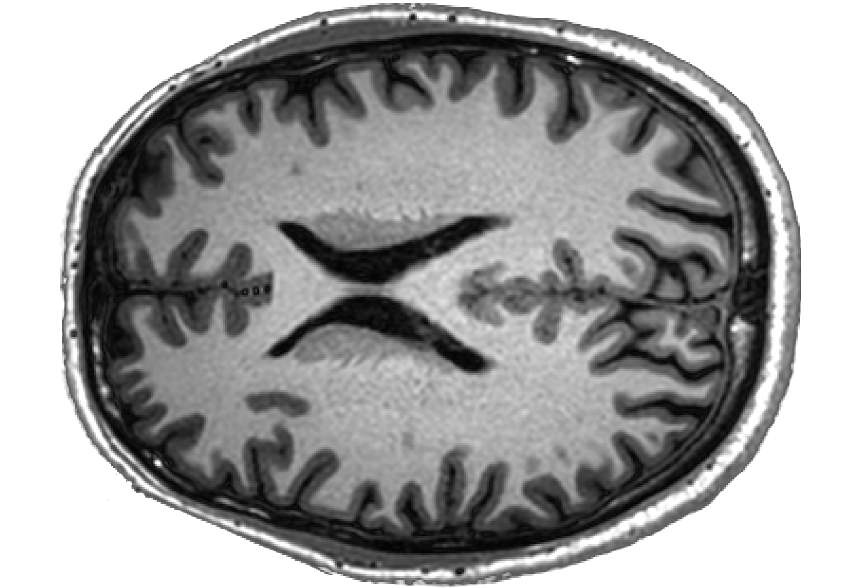
\includegraphics[height=2.3cm]{./graphics/chp1/T1-image-rot-white}
  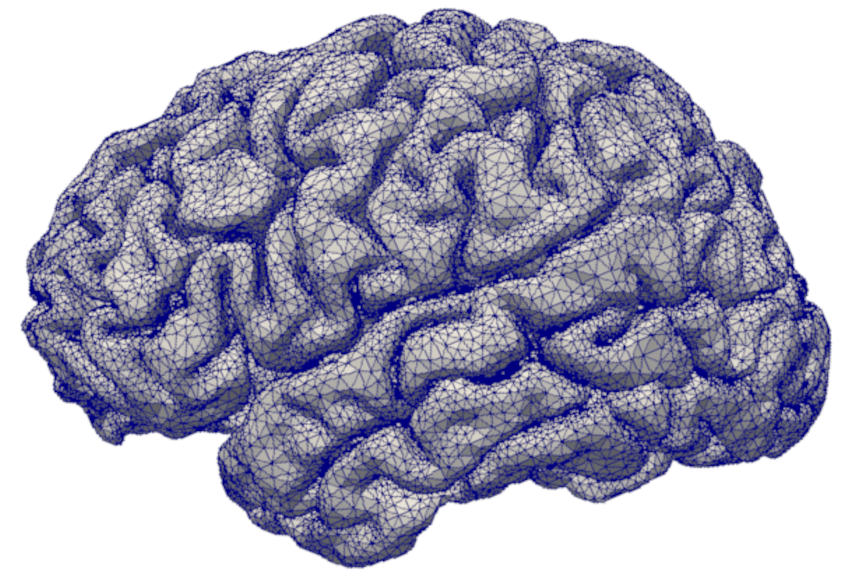
\includegraphics[height=2.3cm]{./graphics/chp1/ernie-volume-64}
  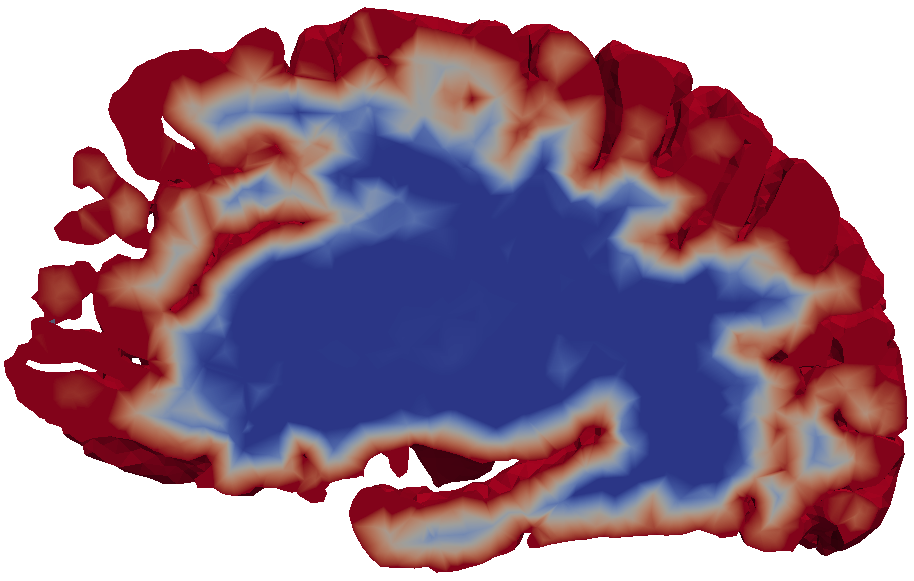
\includegraphics[height=2.3cm]{./graphics/chp1/soltn-t30-crop}
  \hfill
  \end{center}
  \caption{Going from magnetic resonance (MR) images of a human brain
    to a numerical simulation of a biophysical phenomenon. From left
    to right: (a) An MR image of a human brain viewed along the axial
    direction, (b) a finite element mesh extracted from the MR image,
    (c) a snapshot of a tracer distribution simulation over this
    mesh. MR image types are discussed in Chapter~\ref{chp:chp2}}
  \label{fig:chp1:pipeline}
\end{figure}

This book focuses on creating the basic foundation, of computational resources, 
necessary to enable continuum-based modeling of the human brain.  Though we 
don't focus explicitly on the exciting multiphysics applications mentioned 
above, the approach discussed here is generalizable to multiphysics problems.  
You, the reader of this book, will learn how to formulate, set-up and implement 
mathematical and computational models of brain biophysics in patient-specific 
geometries using finite element simulations and MR images (see Figure
\ref{fig:chp1:pipeline}). We will use the evolution and distribution
of a solute concentration due to diffusion as a model problem, and
increase the complexity of the data and techniques involved in the
course of the book. Of course, the process involves several challenges
and pitfalls which will be outlined.

\section{A model problem}

\index{diffusion equation}
Suppose that we aim to study the diffusion of a solute concentration
in a region of the brain. The region $\Omega$ could represent the left
brain hemisphere or a smaller region such as the hippocampus, while
the concentration $u$ could represent an injected tracer used in
imaging (such as gadobutrol~\cite{ringstad2018brain} or
dextran~\cite{iliff2013cerebral}) or possibly a metabolic waste
protein associated with neurodegenerative disease such as
amyloid-$\beta$ or tau. We can describe this model problem by a
time-dependent partial differential equation (PDE): find the
concentration $u = u(t, x)$ at spatial points $x \in \Omega$ and time
points $t > 0$ such that
\begin{subequations}
  \label{eq:diffusion}
  \begin{align}
    \label{eq:diffusion:a}
    u_t - \Div D \Grad u &= f &&\text{ in } (0, T] \times \Omega, \\
    \label{eq:diffusion:b}
    u &= u_d && \text{ on } (0, T] \times \partial \Omega, \\
    \label{eq:diffusion:c}
    u(0, \cdot) &= u_0 && \text{ in } \Omega.
  \end{align}
\end{subequations}
In the diffusion equation~\eqref{eq:diffusion:a}, $u$ is the unknown
field, while $D$ is the diffusion tensor coefficient and $f$
represents any source or sink for the concentration within the
domain. The subscript $t$ denotes the time derivative, $\Div$
represents the divergence and $\Grad$ the spatial gradient. The second
equation~\eqref{eq:diffusion:b} gives a boundary condition: the
function $u_d$ represents a known distribution of the concentration on
the boundary $\partial \Omega$ for all times. The third
equation~\eqref{eq:diffusion:c} gives an initial condition for the
solute concentration: the function $u_0$ represents the known initial
concentration distribution throughout $\Omega$ at $t=0$. The combined
problem \eqref{eq:diffusion} is a complete initial boundary-value
problem and will be our model problem.


\section{On reading this book}
This text does not assume that the reader is well versed in anatomy or in 
neuroscience.  In fact, the bulk of the anatomical familiarity needed to 
successfully follow along with this text is covered in 
Chapter~\ref{sec:chp2:anatomy}.  We have also made liberal use of footnotes and 
citations to inform the reader of additionally interesting, or contextually 
useful, anatomical or physiological details. This text does, however, assume a 
basic knowledge of PDEs. For instance, the diffusion equation 
\eqref{eq:diffusion} is a classical continuum-based PDE with well-known 
behavior in both the mathematical and numerical sense. The reader unfamiliar 
with this equation is advised to first consult an introductory text on solving 
PDEs using the finite element
method~\cite{gockenbach2006understanding,
  langtangen2016solving, langtangen2019introduction,tveito2004introduction}.

The reader is assumed to be comfortable executing commands from a
command line in a terminal window (also canonically referred
to as a command window or command prompt). Terminal commands
will throughout be formatted as:
\terminal{\$ cd ..}
\noindent Commands at the operating-system (OS) level, such as that above,
can differ from OS to OS, and we mainly demonstrate Linux commands
here.

We also assume the reader is familiar with the fundamentals of the
Python programming language or, alternatively, can understand the
syntax well enough to follow the source code that appears throughout;
we will not use any advanced Python programming techniques. We use
Python 3 throughout, and we must therefore make sure that we have Python
version 3.0 or any later version installed. You can check
your Python version by either of the following terminal commands:
\terminal{\$ python {\ddash}version \\
\$ python3 {\ddash}version
}

We will use the Python interface to the FEniCS Project finite
element software~\cite{alnaes2015fenics}, and we assume that the
reader is familiar with the material covered by the FEniCS
tutorial~\cite{langtangen2016solving}.

\section{Data sets and scripts}

\index{mri2fem data sets and scripts}

The data sets and scripts used and described in this book are openly
available and associated with its Zenodo community:
\url{https://zenodo.org/communities/mri2fem/}. 
\begin{itemize}
\item
  The book data set, including MR images, can be downloaded from \\
  \url{http://doi.org/10.5281/zenodo.4386986}~\cite{kent_andre_mardal_2020_4386986}.
\item
  The book scripts can be downloaded from \\
  \url{http://doi.org/10.5281/zenodo.4386998}~\cite{kent_andre_mardal_2020_4386998}.
\item 
  A git repository containing the book and its scripts can be found 
  at: \\ \url{https://github.com/kent-and/mri2fem}.
\end{itemize}
We strongly recommend that you download and unpack these materials
before reading further. We expect to update the Zenodo community with
script updates, updated installation guides and further material as
needed.
 
\section{Other software}
We will use a number of external tools in this book. Most of these
tools are available for a number of operating systems, with separate
installation instructions and dependencies for each system. For the
key external tools, in this book, we provide installation instructions for Linux
Ubuntu (version 20.04, but earlier or later versions might also work
fine). Whenever we refer to an Ubuntu specific terminal command, we
format it as follows:
\ubuntu{\$ sudo apt-get install ... }
\noindent We note that, before installing packages, it can be important to update
the Ubuntu package list. This can be done by the following command:
\ubuntu{\$ sudo apt-get update}
\noindent For other operating systems, we refer to the specific
software documentation for installation instructions.

\section{Book outline}

This book covers the following material. We give an
introduction to brain physiology and brain imaging in
Chapter~\ref{chp:chp2}, as well as survey the software ecosystem
that will take us from MR images to numerical
simulation. In Chapter~\ref{chp:chp3}, our aim is to get up and
running quickly: we step through the entire pipeline from generating a
volume mesh from MR image data to solving our model
problem~\eqref{eq:diffusion} on this mesh. In Chapter~\ref{chp:chp4},
we cover more aspects of meshing including distinguishing between gray and
white matter, merging left and right hemispheres, and adding
parcellation labels. In Chapter~\ref{chap:dti}, we focus on diffusion
tensor imaging (DTI) and demonstrate how we can convert DTI data
to a numerical tensor field. Finally, in Chapter~\ref{chp:chp6}, we
bring everything from Chapters~\ref{chp:chp3} to \ref{chap:dti} together
to present a realistic simulation of anisotropic diffusion in
heterogeneous brain regions. 
 

\chapter{Working with magnetic resonance images of the brain}
\label{chp:chp2}

\section{Human brain anatomy}
\label{sec:chp2:anatomy}
\index{brain anatomy}

The human brain consists of multiple structures, including the large
cerebrum, the smaller cerebellum, and the brain stem. These structures
can easily be identified from MR images of the
brain (Figure \ref{fig:chp2:brain}). The cerebrum is composed of the
left and right hemispheres, which are connected through bundles of
nerve fibers (the corpus callosum).

\index{brain anatomy!white matter}
\index{brain anatomy!gray matter}

There are two main types of brain cells: neurons (or nerve cells) and
glial cells. Each neuron is generally composed of a cell body
(\emph{soma}), a long nerve fiber (\emph{axon}), and other
branching extensions (\emph{dendrites}). The spatial distribution
of the brain cells results in two primary types of brain tissue
matter: white and gray matter.\footnote{In simple terms, neurons have
  a cell body (soma) and branches (axons and dendrites) that extend
  from the cell body. Axons are either covered with a lipid-rich
  (fatty) layer called myelin (myelinated axons) or 
  surrounded by other cells (unmyelinated axons); myelin helps the
  axons conduct electrical signals over long distances. Myelin, being
  fatty, gives off a white-ish color; conversely, unmyelinated axons,
  dendrites, and neural cell bodies, in close proximity to
  microcirculation, appear gray. This is the origin of the terms
  \textit{gray matter} and \textit{white matter}.} White matter mainly consists of
bundles of (myelinated) axons while gray matter includes neuronal cell
bodies, and glial cells. The distribution of white and gray matter in
the cerebrum is shown in Figure~\ref{fig:chp2:brain} (right), which
demonstrates the white matter and the cortical and sub-cortical gray
matter. The sub-cortical gray matter includes a number of important
structures or regions located deep inside the brain, such as~the
hippocampus, basal ganglia and thalamus.
\begin{figure}[t]
  \centering
  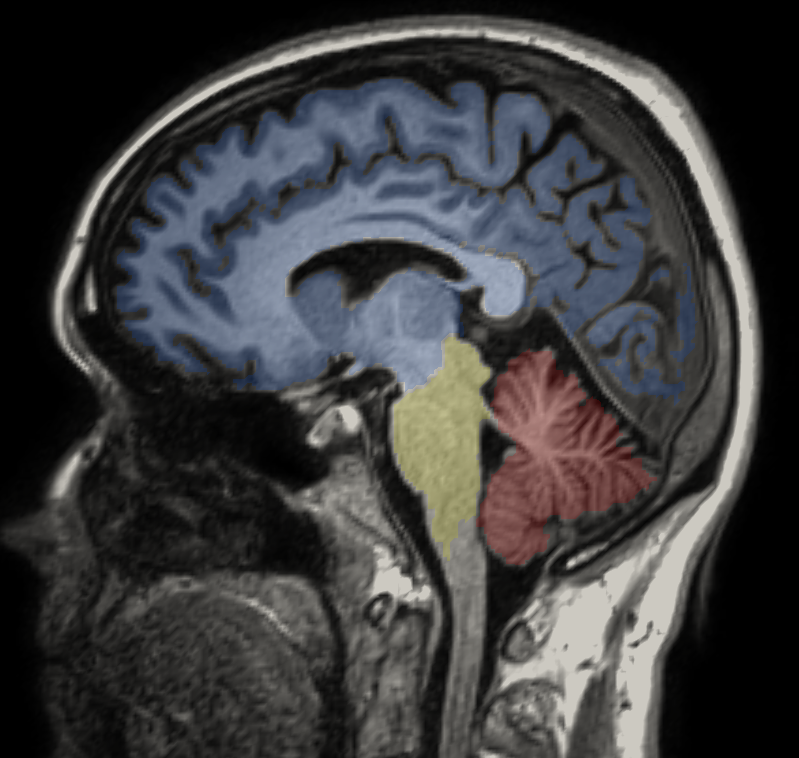
\includegraphics[width=0.48\textwidth]{./graphics/chp2/exp-brain.png}
  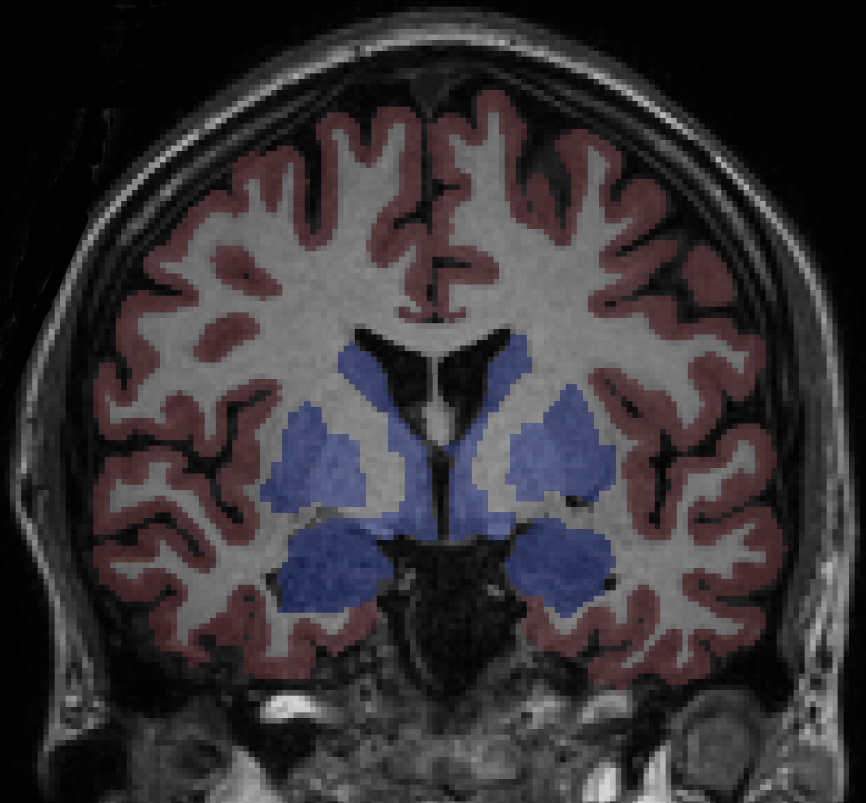
\includegraphics[width=0.48\textwidth]{./graphics/chp2/exp-matters.png}
  \caption{MR images (T1-weighted) of the human brain. Left: A sagittal
    (longitudinal) cross-section of the human brain with the cerebrum
    in blue, the cerebellum in red, and the brain stem in yellow. Right: A coronal
    slice of the brain. The tissue matter
    composition of the cerebrum is marked by color with red denoting
    the cortical gray matter, blue denoting the subcortical gray matter
    and white denoting the white matter. (The colors were added after
    post-processing.)}
  \label{fig:chp2:brain}
\end{figure}

\index{brain anatomy!meninges} \index{brain anatomy!ventricles} The
brain is enclosed and protected by three layers of meninges; the
outermost \emph{dura}, the middle \emph{arachnoid} and the innermost
\emph{pia} membrane. The narrow space between the pial and arachnoid
membranes is filled with cerebrospinal fluid (CSF) and is referred to
as the \emph{subarachnoid space} (SAS). The SAS extends around the
brain and further down along the spinal cord. The SAS is also
connected to the ventricular system, a system of interconnected CSF
compartments surrounded by the brain. The ventricular system consists
of the two lateral ventricles and the third and fourth ventricles,
shown in Figure~\ref{fig:chp2:ventricles}. The thin passage between
the third and fourth ventricle is known as the cerebral aqueduct.
\begin{figure}
  \centering
  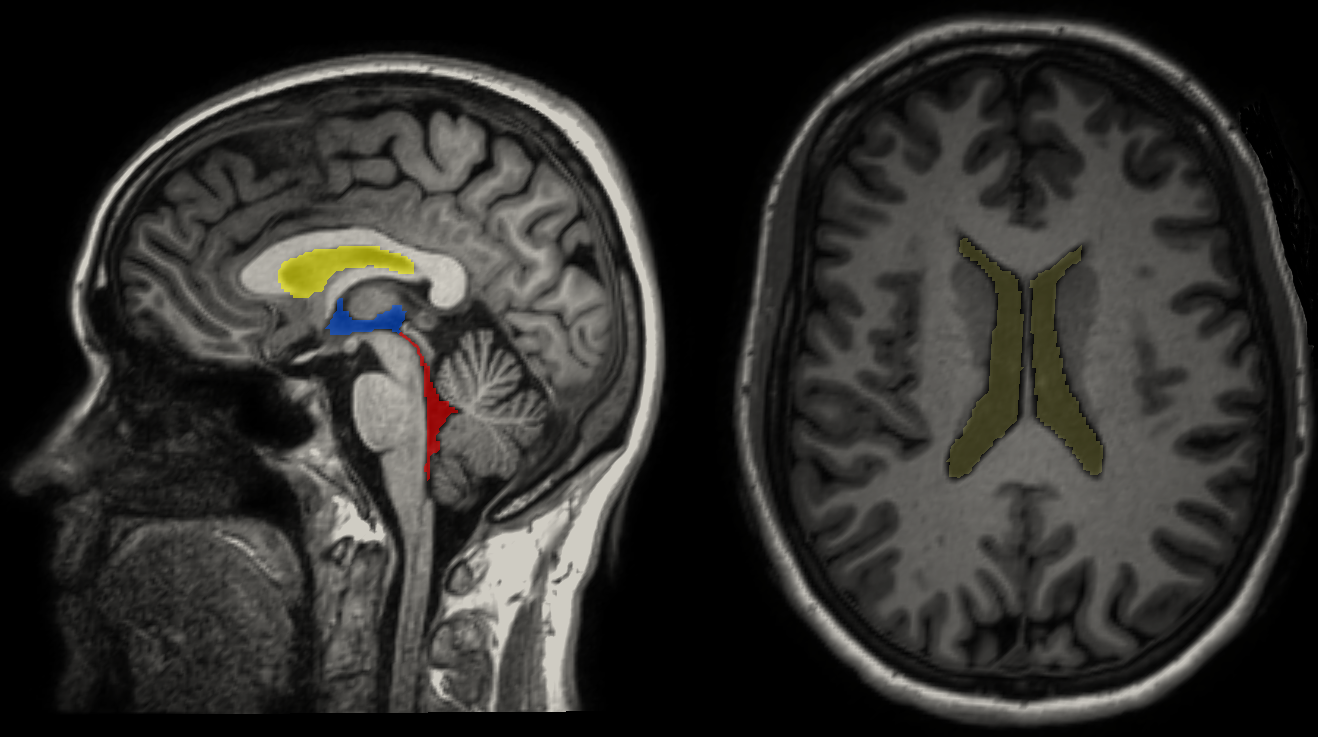
\includegraphics[width=0.98\textwidth]{./graphics/chp2/exp-vent.png}
  \caption{Sagittal (left) and axial (right) MR image cross-sections
    of the brain with the lateral ventricles marked in yellow, the third
    ventricle marked in blue and the 4th ventricle and the aqueduct
    marked in red. The white region surrounding the lateral
    ventricles, on the left, is the corpus callosum. The distinction
    between (cortical) gray and white matter is also clearly visible
    on the right.}
  \label{fig:chp2:ventricles}
\end{figure}

We refer the reader, for example, to \cite{gray2009gray} for a good
introduction to human brain anatomy and \cite{boron2016medical} for a
general introduction to human physiology.

\section{Magnetic resonance imaging}

\index{MRI} \index{MRI!sequence} Magnetic resonance imaging (MRI) is a
rich and versatile technique for the non-invasive medical imaging of
the brain and other organs. The method has its roots in studies of
Isidor Rabi; dating to the early 20th century. Rabi was able to
ascertain information on the rotation and magnetic movements of the
nuclei of atoms and molecules~\cite{thomas2013}. MRI leverages these
types of magnetic properties; specifically for the nucleus of
elemental hydrogen, which is abundant in fat and other
tissues~\cite{berger2002}. An MRI scanner creates a strong magnetic
field, aligning the poles of hydrogen atoms along the scanner's axis.
A radio wave is added to the magnetic field, causing the hydrogen
nuclei to resonate, and different (scanner) slices of the body
resonate differently. Turning off the applied radio frequency induces
the realignment of the hydrogen nuclei with the applied magnetic
field, and this process in turn causes the emission of another radio
wave signal which the MRI scanner measures. The intensity of this last
signal is what we visualize as MRI images \cite{berger2002}.


The MRI method can be used for detailed investigations of tissue
morphology and structure (structural MRI), tissue properties
(e.g.~diffusion-weighted MRI), blood flow (perfusion MRI) as well as
aspects relating to brain function (functional MRI). As detailed
above, an MR image is constructed from the interaction between a
strong magnetic field and radio waves. The specifics of the procedure
can be controlled by manipulating factors that affect this
interaction, such as the magnetic field gradient. A specific set of
changing magnetic gradients is referred to as an MRI \emph{sequence},
which in turn has a number of parameters. We briefly describe a few
key MRI sequences here; the interested reader can find more
information in e.g.~\cite{haacke1999magnetic, payne2017cerebral,
  alexander2007diffusion}.

\subsection{Structural MRI: T1- and T2-weighted images}
\label{sec:T1T2}

\index{MRI!T1}
\index{MRI!T2}
Structural MRI provides high-resolution images of brain anatomy and
can thus give information about the shape, size and composition of
different brain compartments and regions\footnote{Gray matter (cortical) and 
white matter regions are defined vis-a-vis a segmentation and 
parcellation process. Parcellations are discussed in more detail in 
Chapter~\ref{sec:chp4:tools:remove-vent:extraction}}. Examples of structural MRI
sequences include T1- and T2-weighted images, as already
encountered in Figures~\ref{fig:chp2:brain} and
\ref{fig:chp2:ventricles}. Such images are well suited for defining
brain geometry models and will be used extensively for this purpose
(Chapters~\ref{chp:chp3}--\ref{chp:chp4}). A brief introduction to T1-
and T2-weighted images can be found in~\cite{pooley2005fundamental}.

T1- and T2-weighted images correspond to different (groups of) MRI
sequences, each with their own parameters and characteristics. A T1-
or T2-weighted image is a three-dimensional image, typically viewed as
a stack of black and white images of different planes (axial, coronal
or sagittal) of the brain. The colored shading is referred to as the
\emph{signal intensity}; white represents a high signal intensity and
black represents low intensity (with gray tones representing
intermediate values). Both imaging sequences (T1- and T2-weighted)
produce different signal intensities for different types of tissue and
fluids, but the two differ in their dominant intensities.

\begin{figure}
  \centering
  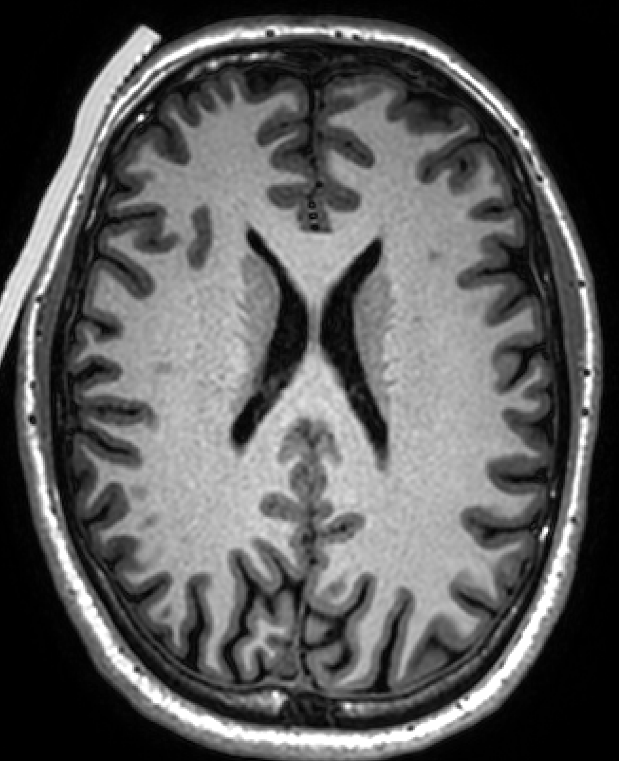
\includegraphics[width=0.415\textwidth]{./graphics/chp2/T1-image.png}
  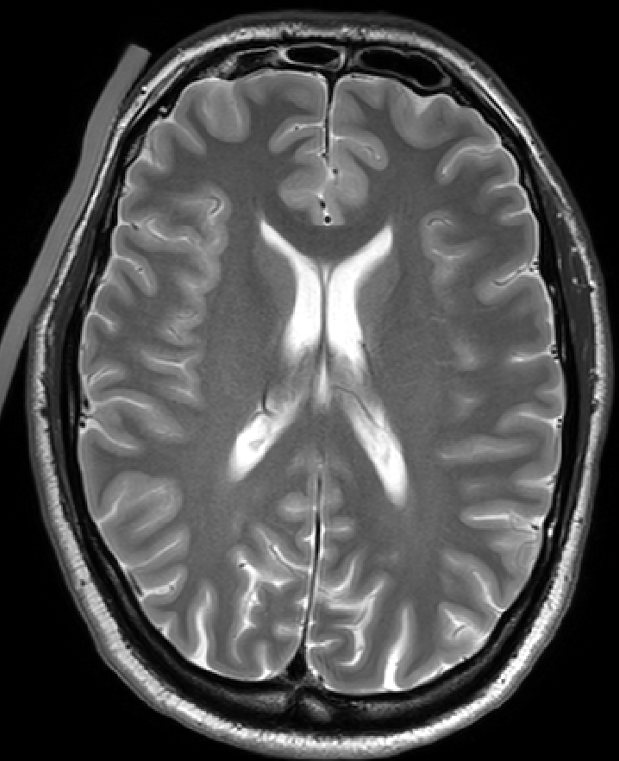
\includegraphics[width=0.415\textwidth]{./graphics/chp2/T2-image.png}
  \caption{T1-weighted image (left) versus T2-weighted image (right).
    In the T1-weighted image, white matter is recognized as light
    gray, whereas the darker gray lining the surface of the brain is
    gray matter. T1-weighted images are used particularly because they
    exhibit a sharp contrast between gray and white matter. The
    T2-weighted image shows the CSF as almost white and provides good
    contrast between the CSF and the brain, but less contrast between
    white and gray matter. Also note that blood is dark in
    T2-weighted images.}
  \label{fig:chp2:t1vt2}
\end{figure}
In T1-weighted images, fat gives off a high intensity signal and
appears white, while fluids give off a low intensity signal and appear
black. Therefore, the brain tissue appears as different shades of gray
with white matter appearing lighter than gray matter
(Figure~\ref{fig:chp2:t1vt2} (left)). T1-weighted images are effective
at differentiating between white and gray matter, but less effective
at distinguishing between, for example, the CSF (black) and the gray
matter (dark gray). In particular, it can be difficult to identify
fluid compartments such as the ventricles, the aqueduct, and SAS from
T1-weighted images alone.

%
\index{brain anatomy!ventricles}
%
In T2-weighted images on the other hand, fluids give off a high
intensity signal and appear white (Figure~\ref{fig:chp2:t1vt2}
(right)). Such images are less effective at distinguishing between
white and gray matter, but can provide good contrast between the CSF
(white) and brain matter (gray). T2-weighted images can thus
supplement data from T1-weighted images for identifying and separating
the ventricles and aqueduct from subcortical gray matter.

\subsection{Diffusion-weighted imaging and diffusion tensor imaging}

\begin{figure}
  \sidecaption
  \centering
  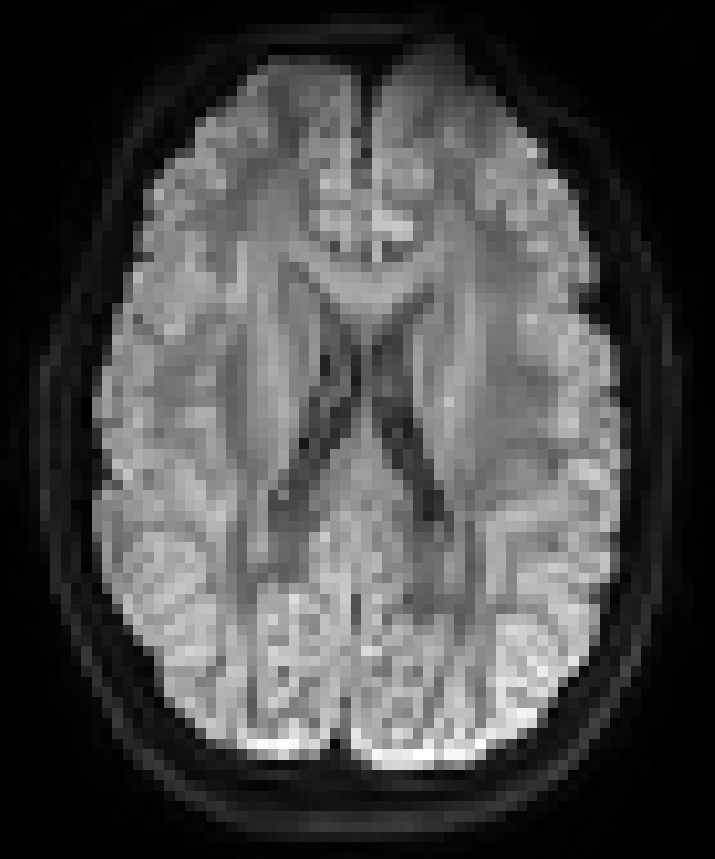
\includegraphics[width=0.49\textwidth]{./graphics/chp2/DTI-slice-image-crop.png}
\caption{A raw, axially-oriented dMRI image of the brain. The 
ventricles (center) appear in lower contrast due to the fast signal decay 
caused by the strongly isotropic diffusion of the water contained within them.} 
\label{fig:chp2:dti}
\end{figure}

%
\index{DTI}
%
Diffusion MRI (dMRI) is an imaging modality that detects water
molecule movement patterns \cite{jeurissen2017,soares2013hitchhiker}.
Both isotropic and anisotropic diffusion coefficients can be
determined. Diffusion tensor imaging (DTI) is a specific type of
diffusion-weighted MRI; Figure~\ref{fig:chp2:dti} shows an example of
a DTI-weighted image. At a high level, a reference signal is used as a
comparison and the DTI imaging process measures the difference in that
reference signal with several follow-up signals. The resulting
sequence provides information about how water diffuses in different
regions of the brain.

More specifically, DTI provides information on both the magnitude and 
(multiple) directions of the movement of molecular water in the brain; that is, 
how water travels. In mathematical terms, DTI provides information regarding 
the diffusion tensor, $D$, in \eqref{eq:diffusion}. In three dimensions, this 
tensor has nine entries and a global representation given by
\begin{equation}
D = \begin{pmatrix}
  d_{11} & d_{12} & d_{13} \\
  d_{21} & d_{22} & d_{23} \\
  d_{31} & d_{32} & d_{33}
\end{pmatrix}.
\end{equation}
Each of the entries $d_{ij}$ can be a function of the position $x \in
\R^3$. We will extract the heterogeneous, anisotropic,
and patient-specific diffusion tensor from DTI 
image data in Chapter~\ref{chap:dti}. DTI has been used extensively to 
study the layout of brain's white matter tracts; these tracts heavily bias 
the movement of water within the brain. We refer the interested reader to
\cite{jeurissen2017}, and the many sources therein, for a discussion
of the more advanced topics related to the field of dMRI techniques.

\section{Viewing and working with MRI datasets}
\label{sec:chp2:tools:viewers}

\subsection{The DICOM file format}
\index{DICOM}

Medical images, including T1, T2 and DTI, are often stored in the
DICOM file format. DICOM stands for \emph{Digital Imaging and
  Communications in Medicine} and is an imaging
standard~\cite{mildenberger2002introduction}. The format stores both
the image itself and a comprehensive set of meta-data, such as
the imaging protocol and patient identification, which enables
consistent and safe usage across different vendors and software
packages. 

The DICOM format gives the output from an MRI scan as a collection of
files arranged in sequences. A given file within a sequence\footnote{Formally, 
the term \textit{MRI sequence} does not refer to an ordered measure (such as a 
sequence in time) but rather to a specific type of pulse sequence or field 
gradient that determines the specific imaging protocol. A T1 
\textit{MRI sequence} produces T1 images, a T2 \textit{MRI sequence} produces 
T2 images, and so forth. Here, when we speak of `a sequence of files' we are 
referring to the order in which the files are produced by the MRI scanner; this 
is typically reflected in the naming of the files such that IM\_0001 would be 
produced before IM\_0002, and so on.} also contains the necessary information 
to inform the viewer what the next (or previous) file in that file sequence is. 
DICOM files are sometimes stored in a binary file named \emp{DICOMDIR} that 
indexes the entire structure of an MRI dataset. 

\subsection{Working with the contents of an MRI dataset}
\label{sec:chp2:viewmri}
\index{DicomBrowser}

A DICOM viewer is an essential component for viewing and working with
DICOM files. A number of DICOM browsers exist, and we will use
DicomBrowser~\cite{dicombrowser}. Currently, DicomBrowser is
available\footnote{https://wiki.xnat.org/xnat-tools/dicombrowser} as a
pre-packaged binary download for several operating systems; the source
code\footnote{https://bitbucket.org/xnatdcm/dicombrowser/src/master/}
is also available. On Ubuntu Linux, DicomBrowser comes pre-packaged
as a Debian package file; this type of file can be installed on
Ubuntu using the command \ubuntu{\$ sudo apt install
  /path to file/my-dicombrowser.deb}
\noindent where you should change `path to file' to the path where the  
DicomBrowser installation file (ending in .deb) has been downloaded and change 
the text of `\emp{my-dicombrowser.deb}' to be the specific filename of the 
DicomBrowser installer package. 

You can then begin the process of extracting sequences from an MRI
data set by launching the DicomBrowser utility with the command:
\terminal{\$ DicomBrowser \&}
\noindent After the DicomBrowser window opens, select
\button{File$\rightarrow$Open} from the top menu bar; a dialogue box
will appear with the heading \button{Select DICOM files}. Navigate to
the directory containing the (example) book dataset and select the directory
titled \emp{\erniedicom}. In this directory, select the file titled
\emp{DICOMDIR}. The main DicomBrowser window should now show a list of
the patients whose data are included in this dataset (in this case
just one patient). In the main window (c.f.~Figure~%
\ref{fig:chp2:dicombrwsr-scr} (left)), click the patient, whose ID starts with 
1.3.46, and then click the symbol to the left of the patient ID to expand the 
entry.

\begin{figure}[h]
  \centering
  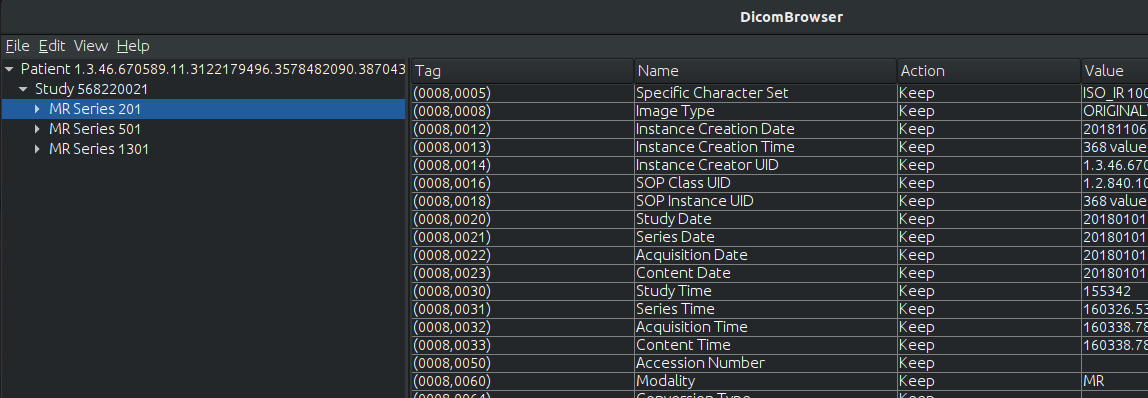
\includegraphics[width=\textwidth]{./graphics/chp2/dicombrowser-d-ext}
  \caption{Example of the DicomBrowser layout and selection of an MR series (\emp{\erniedicom}).} 
  \label{fig:chp2:dicombrwsr-scr}
\end{figure}

A list of studies now appears under the patient ID; generally, a
patient can have several associated studies but the (example) book
dataset contains one study per patient. Expand the study (beginning
with 568) by clicking the symbol to the left. A list of MR series now
fills the main window; many MR series can be contained in a single
study and we see that the \emp{\erniedicom} data contains three series
(201, 501 and 1301), as shown in Figure~\ref{fig:chp2:dicombrwsr-scr}.

Find MR Series 201 and left-click on it. The secondary window now
contains a list of tags, each of which has an associated name, action,
and value (Figure \ref{fig:chp2:dicombrwsr-scr}). Note that tag (0018,
1030)\footnote{Tag identifiers are not standard, and can differ based
  on the MRI scanner manufacturer. Generally, we identify a sequence
  from the Name field by looking for a label containing T1, T2, or
  DTI.} is named `protocol name' and has value T13D; this indicates
that MR Series 201 corresponds to a T1-weighted image sequence. With
`MR Series 201' as the current selection, in the DicomBrowser (left)
window, we can select \button{File$\rightarrow$Save} to extract the
series; a window then appears which provides extraction options. We
would like to extract this series to a directory with a memorable
name; we can do this by changing `-anon' to `-T13D' to signify that
the series we are extracting represents a T1-weighted image in
3D. Also note that DicomBrowser can be used to anonymize the data, as
indicated by the default extension {-anon}, or, in general, to change
DICOM tag values either through the GUI or in scripts.

We can use the same procedure to extract other image sequences. In the
DICOM images in our example dataset, MR Series 501 is a DTI sequence
and MR Series 1301 includes T2-weighted images. We have already
extracted all three series present in the sample \emp{DICOMDIR} into
the (example) book dataset. Image series 201 has been extracted to
\emp{\erniedicom/T13D}, image series 1301 has been extracted to
\emp{\erniedicom/T23D}, and image series 501 has been extracted to
\emp{\erniedicom/DTI}. We note that \emp{\erniedicom/DTI} also
contains some non-image files; these files are not in the
\emp{DICOMDIR} data but will be generated and discussed in
Chapter~\ref{chap:dti}.

\section{From images to simulation: A software ecosystem}
\label{sec:chp2:software-ecosystem}
In this section, we provide a brief overview of the software tools that 
comprise the pipeline used in this book. We will extract data from clinical
images, segment the data, extract and work with diffusion tensor
information, generate a finite element mesh, and bring all of this
together to solve a partial differential equation. Along
the way, we will need additional tools for miscellaneous
objectives, such as file conversion and visualization. A visual
representation of the patient-specific pipeline from MRI-images to
finite element simulations is shown in Figure
\ref{fig:chp2:imaging-pipeine-overview}.

\begin{figure}
\centering
 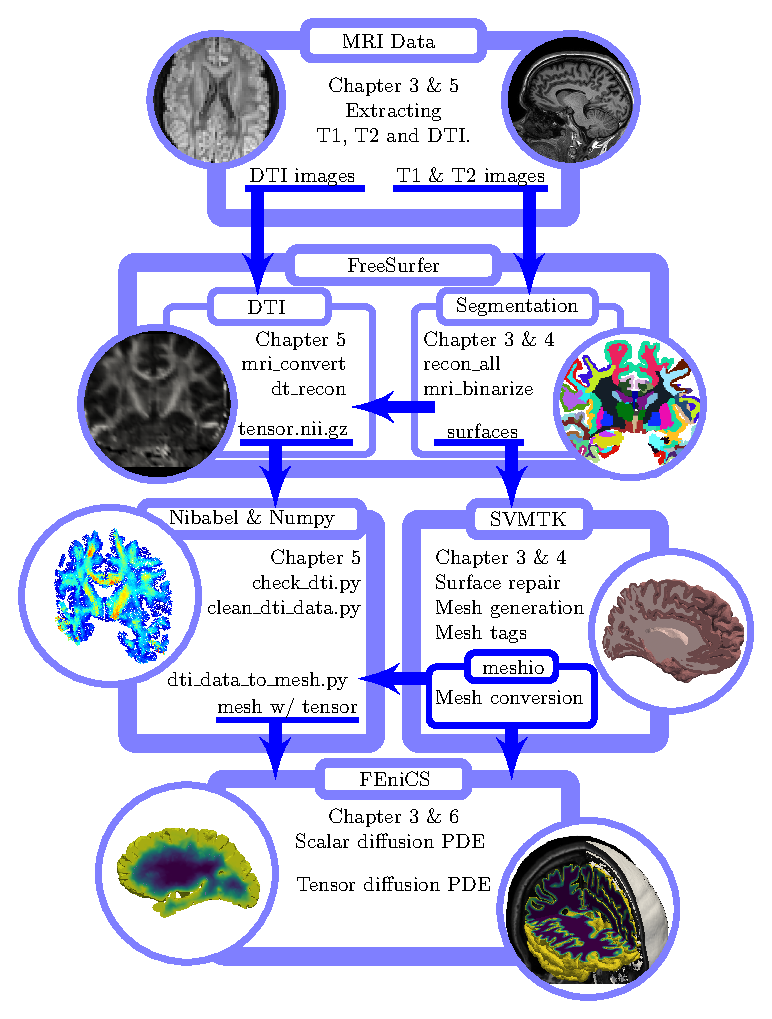
\includegraphics[width=0.95\textwidth]{./graphics/chp2/pipeline-overview.pdf} 
  \caption{Overview of the imaging, segmentation, meshing, simulation
    and visualization pipeline. T1, T2, and DTI images have already
    been discussed.  Freesurfer and segmentation are discussed in
    Section~\ref{sec:chp2:tools:freesurfer}. Nibabel and Numpy are
    Python libraries that are used for neuroimaging applications and
    convenient manipulation of tensors, respectively. {\svmtk} is a
    computational geometry package, written for this book, which is
    specialized for creating brain meshes and {\fenics} is a Python
    library for high-performance finite element method computations.}
  \label{fig:chp2:imaging-pipeine-overview}
\end{figure}

\subsection{FreeSurfer for MRI processing and segmentation}
\label{sec:chp2:tools:freesurfer}
\index{FreeSurfer}
\index{segmentation}

FreeSurfer \cite{dale1999cortical} is an open-source software suite
for the segmentation (identification of different brain regions), processing,
visualization, and analysis of human brain MR images. FreeSurfer is
well established, well documented, and widely used and we refer to the
FreeSurfer website for extensive documentation, online tutorials,
support, an overview of publications and general installation
instructions \cite{freesurfer}. Generally, all \freesurfer{} commands
also have extensive documentation available via \emp{-{}-help}. At the time of 
writing, FreeSurfer provides step-by-step installation guides for 
Linux\footnote{\url{https://surfer.nmr.mgh.harvard.edu/fswiki//FS7\_linux}}
and Mac\footnote{\url{https://surfer.nmr.mgh.harvard.edu/fswiki//FS7\_mac}} 
Below, we discuss the Linux installation process, for the sake of completeness. 

To install FreeSurfer on Ubuntu Linux, we suggest downloading the most
recent FreeSurfer tar archive\footnote{See for example
  \url{https://surfer.nmr.mgh.harvard.edu/fswiki/FS7\_linux}} locally,
for instance under \emp{/home/me/local/src}. If the name of this file
is \emp{freesurfer.tar.gz}, unpack the archive via \ubuntu{\$ tar
  -zxvpf freesurfer.tar.gz}
\noindent The next step is to configure your environment for using
FreeSurfer. If your FreeSurfer archive has been unpacked at
\emp{/home/me/freesurfer}, you can configure your FreeSurfer
environment manually by adding the following lines at the end of the
file named \emp{.bashrc} in your home directory:
\begin{lstlisting}[style=bashStyle]
export FREESURFER_HOME=/home/me/freesurfer 
export SUBJECTS_DIR=$FREESURFER_HOME/subjects 
source $FREESURFER_HOME/SetUpFreeSurfer.sh
\end{lstlisting}
  


\index{Freeview}
\noindent The {FreeSurfer} programming team requires that each user
acquire a license file to use the software; the license file is free,
and to acquire it, follow the registration directions at the FreeSurfer
website \cite{freesurfer}. Finally, FreeSurfer comes packaged
with the Freeview visualization tool. Test Freeview (and your
FreeSurfer installation) by opening a new terminal (noting the
FreeSurfer environment commands appearing on top), and typing:
\terminal{\$ freeview \&}
\noindent to open the Freeview user interface.

We will use the command \emp{dt\_recon} in FreeSurfer, which has
additional requirements: tcsh\footnote{tcsh refers to a specific type
  of Unix shell. A Unix shell is a command-line interpreter; many such
  shells can be used in a Unix environment (such as Ubuntu Linux).}
and FSL. The installation of tcsh can be done from the terminal with
the following command lines: \ubuntu{\$ sudo apt update \\ \$ sudo apt
  install tcsh}

FSL is a comprehensive library for functional MRI, MRI, and DTI brain
imaging data~\cite{jenkinson2012fsl}, and we refer the reader to its
website for installation instructions.\footnote{See
  https://fsl.fmrib.ox.ac.uk/fsl/fslwiki/FslInstallation.} Note that
FSL, like FreeSurfer, requires a license to be operational.

\subsection{NiBabel: A python tool for MRI data}
\label{sec:chp2:tools:nibabel-numpy}

The Python module NiBabel~\cite{brett_matthew_2020_4295521} provides read and write
access to several neuroimaging file formats. The module is part of
NIPY, \footnote{See \url{https://nipy.org/}.} a community for neuroimaging
data analysis via Python. NiBabel can be installed using pip, for example, via the  
following terminal command:
\ubuntu{\$ sudo apt install python3-pip \\
\$ sudo pip3 install nibabel}
\noindent We will use Nibabel to work with image data in Python in 
Chapter~\ref{chp:chp4} and onwards.

\subsection{\svmtk{} for volume mesh generation}
\label{sec:chp2:tools:meshing:svmtk}
\index{SVM-Tk}

The Surface Volume Meshing Toolkit (\svmtk{}) generates meshes with
subdomains based on surfaces and segmentations provided by
FreeSurfer. In particular, \svmtk{} provides a Python-based interface
to the Computational Geometry Algorithms Library
(CGAL)~\cite{fabri2000design} and provides tools for both fixing and
marking surfaces to enable a relatively robust mesh generation for the
various compartments of the brain. We refer to the \svmtk{}
documentation\footnote{See https://github.com/SVMTK/SVMTK.} for
general installation instructions, including a detailed list of
dependencies (including CGAL and a number of packages available,
e.g.~through the Ubuntu package manager).

\subsection{The FEniCS Project for finite element simulation}
\label{sec:chp2:tools:fenics}
\index{FEniCS}
\index{FEniCS!tutorial}

We will use the open-source FEniCS Project~\cite{alnaes2015fenics,
  logg2012automated} as our finite element software. FEniCS includes
both a C++ and a Python interface; we will use the Python interface
throughout. Extensive documentation, support, an overview of
publications, and general installation instructions can be found on
the FEniCS Project website \cite{fenicsproject}. In particular, we
strongly encourage the reader to become familiar with FEniCS and the
finite element method via the introductory FEniCS tutorial
\cite{langtangen2016solving}.

There are many ways to install the FEniCS Project software, including
the use of Docker images, using pre-built Anaconda packages, or from
source. Two simple ways of installing FEniCS are via Docker
images (see the FEniCS Project
website\footnote{\url{https://fenicsproject.org/download/}}) and via Ubuntu
package managers. For the latter, use the following terminal commands:
\terminal{%
\$ sudo apt-get install software-properties-common \\
\$ sudo add-apt-repository ppa:fenics-packages/fenics \\
\$ sudo apt-get update \\
\$ sudo apt-get install {\ddash}no-install-recommends fenics
} 


\subsection{ParaView and other visualization tools}
\label{sec:chp2:paraview}

\index{ParaView} We recommend using ParaView~\cite{ahrens2005paraview}
to visualize the simulation results and other meshing objects that we
discuss throughout the book. For installation instructions, see the
ParaView website\footnote{See \url{https://www.paraview.org/}.}. On
Ubuntu Linux, ParaView can be installed with the following terminal
command: \ubuntu{\$ sudo apt-get install paraview}
\noindent After installation, ParaView can be launched with
\terminal{\$ paraview \&}

An optional but useful tool for visualizing surfaces (in the form
of surface STL files) is Gmsh~\cite{geuzaine2009gmsh}. For installation
instructions, see the Gmsh
website.\footnote{See \url{http://gmsh.info/\#Download}.} On Ubuntu Linux,
Gmsh can be installed with the following terminal command:

\ubuntu{\$ sudo apt-get install gmsh}

For quick plotting in Python, the Python package Matplotlib
is very convenient~\cite{hunter2007matplotlib}. The pyplot module of
Matplotlib can be imported in a Python script (as any other Python
module) as:
\begin{python}
import matplotlib.pyplot as plt
\end{python}

\subsection{Meshio for data and mesh conversion}
\label{sec:chp2:meshio}

\index{meshio}
We recommend using meshio \cite{schlomer2020nschloe} for conversion
between computational mesh formats. The meshio suite can convert
between various unstructured mesh formats, for instance, between the
CGAL medit file format (.mesh) and the FEniCS mesh format (.xml or
.h5). We suggest using the pip installer to install meshio\footnote{See \url{https://pypi.org/project/meshio/}.} for example, via typing the following in the terminal:
\ubuntu{\$ sudo pip3 install meshio[all]}

\subsection{Testing the software pipeline}
\label{sec:chp2:tools:testing}

To verify that all software dependencies are correctly installed, we
provide a test script (in \emp{mri2fem/chp2}); the test script can 
be executed with the command:
\terminal{\$ python3 test\_book\_software.py}
The script will check each software dependency and output a response indicating 
whether it is installed or not. 
If the software is not installed, the response provides a detailed description of ways to correctly install it, including links to installation guides: 
\terminal{Checking FEniCS installation.\\\\
\hspace*{1cm}	FEniCS is not installed\\
\hspace*{1cm}	Follow the installation guide at\\
\hspace*{1cm} 	https://fenicsproject.org/
}
If the software is installed, the response is a single-line response confirming that the software is installed:
\terminal{Checking FEniCS installation. => FEniCS installed}



\chapter{From T1 images to numerical simulation}
\label{chp:chp3}

The goal of this chapter is to enable numerical simulation over a
brain region defined from structural MR images. To address this
challenge, we first demonstrate how to generate a high quality mesh of
a brain hemisphere from T1-weighted MR images using the tools
introduced in Chapter~\ref{chp:chp2}. Next, we show how to define a
finite element discretization of the diffusion
equation~\eqref{eq:diffusion} over this mesh to simulate the influx of
an injected tracer.

\section{Generating a volume mesh from T1-weighted MRI}
\label{sec:chp3:tools}

To generate a mesh from an MRI data set including T1-weighted images,
we follow three main steps:
\begin{enumerate}
\item
  Extract a T1-weighted image series from the MRI dataset,
\item
  Create (boundary) surfaces from the T1-weighted images using FreeSurfer,
\item
  Generate a volume mesh of the interior using FreeSurfer along with \svmtk.
\end{enumerate}
We will consider each of these steps in order and encourage the
reader to ensure that FreeSurfer is installed and configured (see
Chapter~\ref{sec:chp2:tools:freesurfer}) before proceeding. Step 2 can
be particularly time consuming, likely with FreeSurfer segmentation
and reconstruction run times of up to 24 hours.
While we provide already processed files in the tarball that accompanies
the book, we encourage the reader to try these steps.
 
\subsection{Extracting a single series from an MRI dataset}

\index{DicomBrowser}
To extract a single MR series from an MRI dataset or a DICOM database,
we can use the DicomBrowser graphical interface or FreeSurfer command
line tools. The first option, using the DicomBrowser graphical
interface to extract a T1-weighted image series, is described in
Chapter~\ref{sec:chp2:viewmri} with the book data set as an example,
and the resulting image series can be found under \ernieT1 in
the book data set. The second option is described in
Chapter~\ref{sec:chp3:advanced} at the end of this chapter.

\subsection{Creating surfaces from T1-weighted MRI}
\label{sec:chp3:surfaces}

\index{FreeSurfer}
\index{FreeSurfer!\emp{recon-all}}
\index{MRI!T1}

The next step is to create surfaces, representing, for example, the
interface between the pial membrane and the surrounding cerebrospinal
fluid (CSF), referred to here as the pial surface, or the interface
between white and gray matter, from the T1-weighted MRI series just
extracted. We will use FreeSurfer for this task, and as an example, we
will extract the pial surface surrounding the left hemisphere of a
brain.

To conduct a full image stack segmentation and surface reconstruction,
we take advantage of the FreeSurfer command \emp{recon-all}. This
command is compute-intensive, with run times likely up to 24
hours. To invoke \emp{recon-all}, we select one of the T1 DICOM files:
for instance, in~\emp{\ernieT1}, we can pick \emp{IM\_0162}. Next, we
decide on a subject identifier for the FreeSurfer pipeline; we choose
to name this example subject ernie. We are now ready to launch
\emp{recon-all}\footnote{This is a good thing to do on a separate
  core or overnight.}

\terminal{\$ cd \emp{\ernieT1} \\
  \$ recon-all -subjid ernie -i IM\_0162 -all}

The results of \emp{recon-all} will be output to the folder
\emp{SUBJECTS\_DIR/ernie}, where the environment variable
\emp{SUBJECTS\_DIR} defaults to the \emp{subjects} folder under
\emp{FREESURFER\_HOME} (see
Chapter~\ref{sec:chp2:tools:freesurfer}). For convenience, this output
is also included in the book data set, under \emp{\ernieoutput}. If we
inspect the contents of this directory we will see several
subdirectories. Some important subdirectories are
\begin{itemize}
\item \emp{/stats}, contains files providing statistics derived during segmentation;
\item \emp{/mri}, contains volume files generated during segmentation; and
\item \emp{/surf}, contains surface files generated during segmentation.
\end{itemize}

%
\index{Freeview}
%
To view the generated surface files, we focus on the \emp{/surf}
directory, and launch Freeview (see
Chapter~\ref{sec:chp2:tools:freesurfer}):
\terminal{\$ cd \ernieoutput/surf\\
\$ freeview \&}
\noindent Targeting the pial surface that surrounds the left brain
hemisphere as an example, select \button{File$\rightarrow$Load Surface}
from the command bar, and then select the file titled \emp{lh.pial}
(where \emp{lh} refers to left hemisphere and \emp{pial} denotes the pial
surface). After a moment, the view windows will be populated with 2D
surface slices shown as curves, in addition to a reconstructed 3D
image of the pial surface (Figure~\ref{fig:chp3:freeview-scr}).
\begin{figure}%\sidecaption
  \centering
  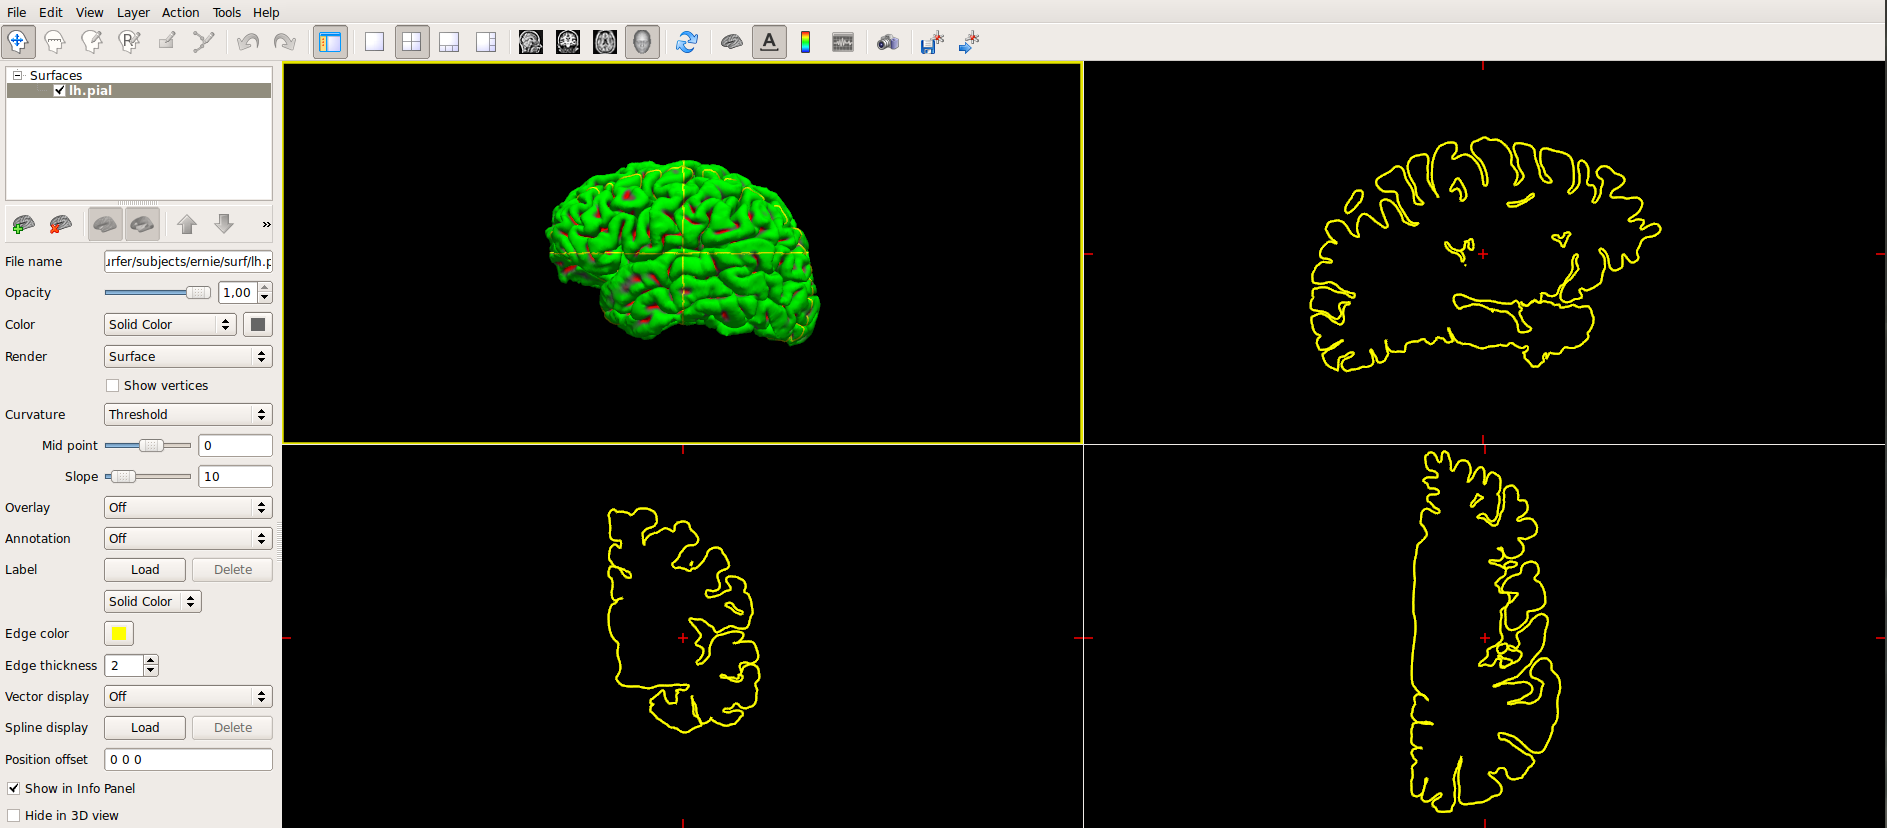
\includegraphics[width=0.95\textwidth]{./graphics/chp3/freeviewexscr}
  \caption{Freeview visualization of the pial surface of a single
    brain hemisphere extracted from T1 images via FreeSurfer.}
  \label{fig:chp3:freeview-scr}
\end{figure}

%
\index{FreeSurfer!\emp{mris\_convert}}
%\index{STL}
%\index{ParaView}
%
To work further with this surface, we use the FreeSurfer tool
\emp{mris\_convert} to convert the binary surface file into the STL
format~\cite{roscoe1988stereolithography}. STL is a widely used format
representing the surface discretely in terms of vertices, triangles
and normals. Generally, \emp{mris\_convert} is used to handle the
conversion between different surface formats. For instance, in the
directory \emp{\ernieoutput/surf}, we can run

\terminal{\$ mris\_convert ./lh.pial pial.stl}

\noindent to create the file \emp{lh.pial.stl} in the current
directory. The resulting file can be opened in several different
programs, for instance, ParaView or Gmsh.

\subsection{Creating a volume mesh from a surface}
\label{subsec:chp3:mesh-creation}

%
\index{mesh generation}
\index{SVM-Tk}
\index{SVM-Tk!\emp{Domain}}
\index{SVM-Tk!\emp{Surface}}
\index{SVM-Tk!\emp{create\_mesh}}
\index{SVM-Tk!\emp{save}}
%
The third step of our initial meshing pipeline is to generate a mesh
of the volume bounded by the surface representation. We will use the
tailored package \svmtk{} (see
Chapter~\ref{sec:chp2:tools:meshing:svmtk}) to convert from the STL
surface representation to a volume mesh. The Python script below (
\emp{mri2fem/chp3/surface\_to\_mesh.py} in the book scripts)
demonstrates the fundamentals of this process. The script (and all
similar scripts in the following) can then be run from there as
\terminal{\$ python surface\_to\_mesh.py}
Recall that Python version 3 is required.  If you have more than one version 
of python installed on your machine you may need to use `python3' in the 
above, and all further commands, instead of the `python' directive; this will 
explicitly specify which version of Python should be used to execute the 
script at hand.  %
%
The script \pythoninline{surface\_to\_mesh.py} defines a Python function, 
named \pythoninline{create\_volume\_mesh}, within it that can be called as
\newpythonsnippet{chp3}{surface_to_mesh.py}{15}{16}

\noindent The function itself reads
\newpythonsnippet{chp3}{surface_to_mesh.py}{0}{12}

\noindent Given an input STL filename (\pythoninline{stlfile}), an
output mesh filename with the \pythoninline{mesh} suffix
(\pythoninline{meshfile}), and an optional mesh resolution
(\pythoninline{resolution}, defaulting to 16), the script creates an
\svmtk{} \pythoninline{Domain} object, generates a volume mesh from the
surface via the call to \pythoninline{create\_mesh}, and saves this
mesh in the \pythoninline{.mesh} format to the output mesh file. The
mesh resolution parameter determines the maximum size of a tetrahedron
in the volume mesh (relative to the overall bounding box length for
the input surface): the higher the value, the higher the resolution,
that is, the smaller the volume of each element in the volume mesh
generated. Figure \ref{fig:chp3:ernie-volume-mesh} shows meshes with
\pythoninline{resolution = 16} (left) and \pythoninline{resolution =
  64} (right). Mesh generation can be a costly operation, with higher
run times (on the order of seconds to minutes) for higher resolutions.
\begin{figure}
  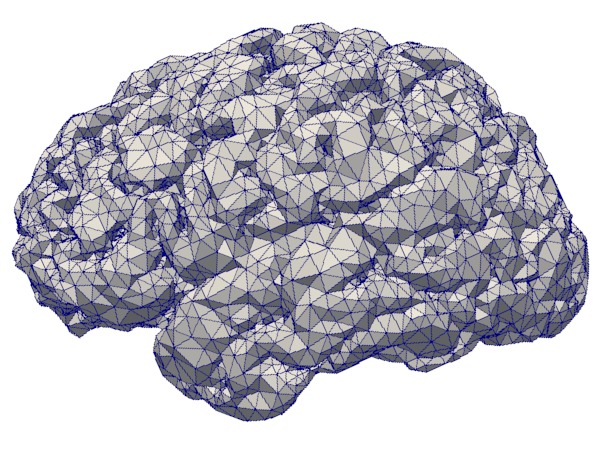
\includegraphics[width=0.49\textwidth]{./graphics/chp3/ernie-volume-16-r.png}
  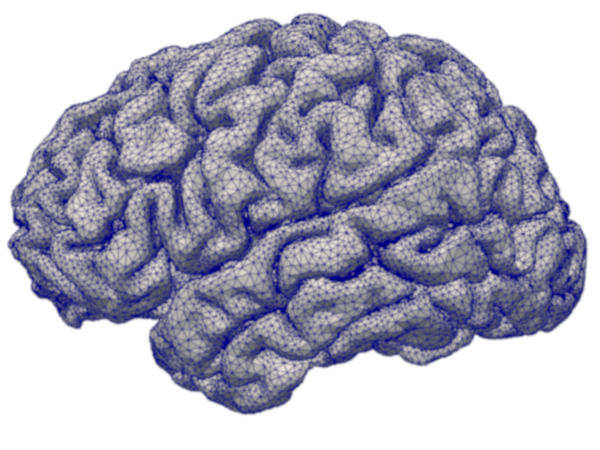
\includegraphics[width=0.49\textwidth]{./graphics/chp3/ernie-volume-64-r.png}
  \caption{Volume meshes of a left brain hemisphere produced by
    {\svmtk} from STL surface files, with lower (left) and higher
    (right) mesh resolutions.}
  \label{fig:chp3:ernie-volume-mesh}
\end{figure}

\index{meshio}
\index{ParaView}
The \emp{.mesh} format is the standard mesh format for \svmtk{} and
CGAL. However, it is not native to \fenics{}, and we therefore need to
convert the mesh to a \fenics-supported file format (for example .xml, .xdmf,
.h5). The Python package meshio (see~Chapter
\ref{sec:chp2:meshio}) is well suited for this purpose and can
convert between many different input and output mesh formats. For
instance, to convert to the FEniCS .xdmf format, we can run
\terminal{\$ meshio-convert lh.mesh lh.xdmf}
\noindent The .xdmf file can then be viewed in, for example, ParaView.

\section{Improved volume meshing by surface preprocessing}
\label{sec:chp3:improved-volume-meshing}
In the previous section, we stepped through the main pipeline for
generating a volume mesh from MR images. However, the brain surfaces
generated from T1 images often have a number of weaknesses:
\begin{itemize}
\item The surfaces can have unphysiologically sharp corners,   
\item The surfaces can include triangles with very large aspect ratios, 
\item The surfaces can have topological defects such as holes, and
\item The surfaces can self-intersect or overlap with other surfaces.   
\end{itemize}
These defects can cause the volume mesh generation to fail or result
in low-quality meshes that are not suitable for numerical
simulation. Therefore, surface preprocessing is often required to
enhance surface quality prior to generating volumetric meshes. Here,
we outline three main aspects of surface preprocessing: remeshing,
smoothing and separation. The enhanced STL surfaces can then be
directly inserted into the volume mesh generation described above in
Chapter~\ref{subsec:chp3:mesh-creation}.

\subsection{Remeshing a surface}
\label{subsubsec:chp3:mesh-creation:remeshing}

To increase surface or volume mesh quality, we can remesh the original
surface representation. The remeshing can, for instance, reduce the
frequency of mesh cells that are overly distorted and reduce the
density of vertices with large numbers of connected edges.

\svmtk{} includes utilities for remeshing surface files, and we can
remesh our original surface \emp{lh.pial.stl}, for example, via the
following script (included as \emp{mri2fem/chp3/remesh\_surface.py} in
the book scripts). We define a short Python function
\pythoninline{remesh_surface} that can be called as
\newpythonsnippet{chp3}{remesh_surface.py}{16}{17}
%
\index{SVM-Tk!\emp{Surface}}
\index{remeshing}
\index{SVM-Tk!\emp{save}}
%
\noindent The function itself reads
\newpythonsnippet{chp3}{remesh_surface.py}{0}{15}

\noindent Here, we read the input STL file as an \svmtk{}
\pythoninline{Surface}, and remesh using
\pythoninline{isotropic\_remeshing}, before saving the remeshed
surface again as an STL file. We can specify more iterations and
produce a finer mesh by increasing the integer value of
\pythoninline{n}; we mention that \pythoninline{n} should not be thought of as 
an `average inverse cell size' but only as a qualitative parameter such that 
higher values produce, generally, finer meshes.  On the other hand, the floating 
point value of \pythoninline{L} corresponds to a quantitative mesh parameter; %
%
%The floating point value of 
\pythoninline{L} indicates the maximum edge length of a mesh cell. Surfaces 
generated by FreeSurfer are typically in millimeters (mm), and the volume meshes
inherit this unit. The Boolean
\pythoninline{do\_not\_move\_boundary\_edges} defines whether \svmtk{}
is allowed to move the boundary vertices during the remeshing
procedure (\pythoninline{False}) or not (\pythoninline{True}). It is
generally advised to allow boundary vertices to move, since requiring
these to be fixed can cause the remeshing to fail.

\index{ParaView}
Figure \ref{fig:chp3:ernie-remesh} shows the result
\emp{lh.pial.remesh.stl} with three remeshing iterations on the raw
input file \emp{lh.pial.stl}. The figure has been zoomed in to draw
attention to local feature differences. Both files were viewed
and visualized in ParaView.
\begin{figure}
  \centering
  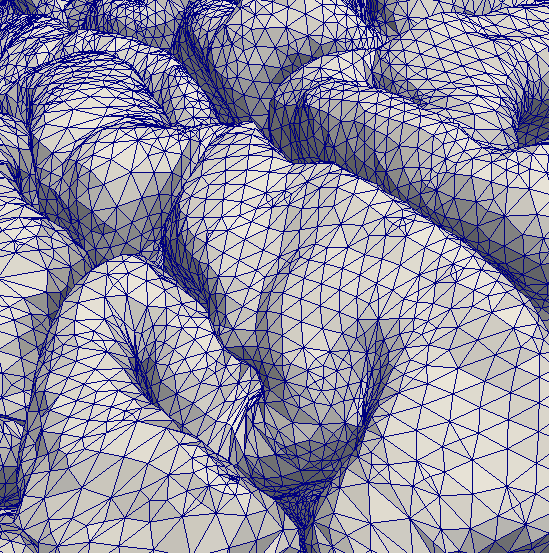
\includegraphics[width=0.49\textwidth]{./graphics/chp3/raw-stlmesh.png}
  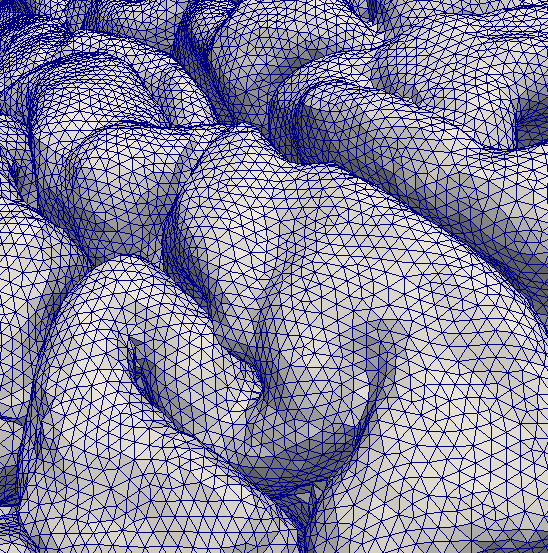
\includegraphics[width=0.49\textwidth]{./graphics/chp3/remesh-stlmesh.png}
  \caption{Original (left) pial surface and (right) after remeshing with \svmtk{}}
  \label{fig:chp3:ernie-remesh}
\end{figure}


\subsection{Smoothing a surface file}
\label{subsubsec:chp3:mesh-creation:smoothing}

To reduce the presence of non-physiological features such as sharp
corners, it may be advantageous to smoothen the surfaces prior to
volume meshing. \svmtk{} also includes utilities for smoothing surfaces, as
we demonstrate in the script below (included as
\emp{mri2fem/chp3/smooth\_surface.py} in the book scripts), using
our remeshed surface \emp{lh.pial.remesh.stl} as sample input.  It is worth 
noting that surface smoothing operations alter the position of existing 
vertices; in particular, smoothing does not alter the number of elements in 
the mesh.  %
%
\index{SVM-Tk!\emp{Surface}}
\index{smoothing}
%
Again, we define a short Python function
\pythoninline{smoothen\_surface} that can be called as
\newpythonsnippet{chp3}{smooth_surface.py}{19}{20}
\noindent The function itself reads
\newpythonsnippet{chp3}{smooth_surface.py}{0}{17}

The Boolean variable \pythoninline{preserve\_volume} determines
whether a shrinkage-preventing \cite{taubin1995curve} Taubin smoothing 
(\pythoninline{True}) or a Laplacian 
smoothing (\pythoninline{False}) process should be used.  From a conceptual
point of view, Taubin smoothing is essentially a local smoothing
iteration followed by a local `swelling' operation that aims to prevent 
any shrinkage in the volume of the original patch, whereas Laplacian smoothing 
consists only of local smoothing operations and the volume of the original
patch might not be preserved \cite{taubin1995curve}. Between the two, we
recommend Taubin smoothing. The integer value \pythoninline{n}
sets the number of times the smoothing process should take place. Higher
values will produce a smoother mesh; however, too high of a value may
result in a loss of resolution in brain features, such as the sulci and
gyri (grooves and bumps), on the brain surface. Finally, the floating
point value \pythoninline{eps} determines the strength of the
smoothing operation for each smoothing iteration, and should be in the
interval $[0, 1]$ with $0.0$ ($1.0$) indicating no (full)
smoothing.
\begin{figure}
  \centering
  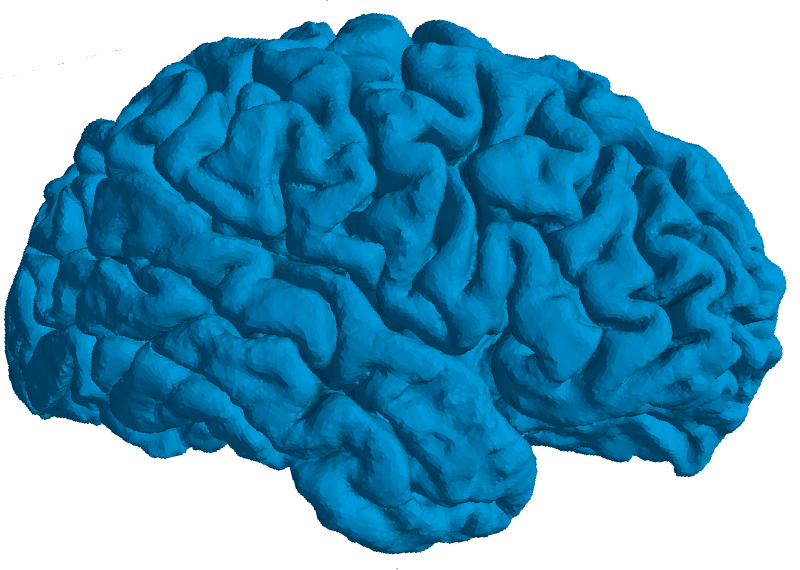
\includegraphics[width=0.30\textwidth]{./graphics/chp3/unsmoothed.png}
  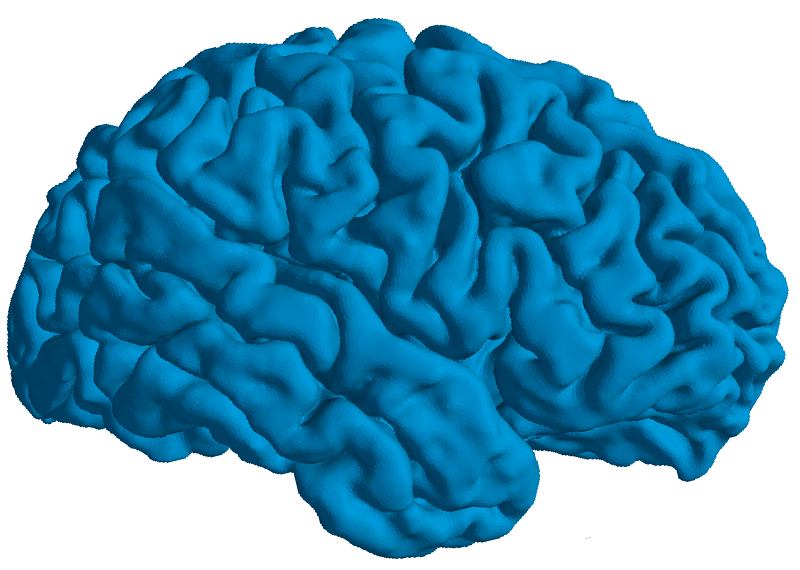
\includegraphics[width=0.30\textwidth]{./graphics/chp3/taubin-smoothed-10.png}
  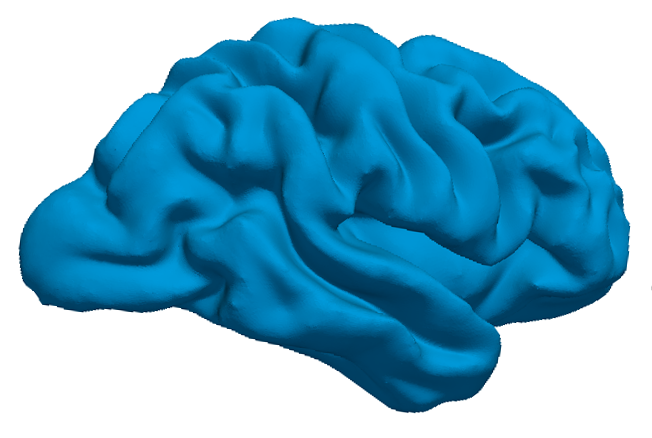
\includegraphics[width=0.30\textwidth]{./graphics/chp3/oversmoothing.png}
  \caption{Surface smoothing: original pial surface 
    (\emp{lh.pial.remesh.stl}, left), after Taubin smoothing with
    {\svmtk} (\emp{lh.pial.smooth.stl}, middle), and Laplacian over-smoothing (right).}
  \label{fig:chp3:ernie-smoothing}
\end{figure}
%
\index{ParaView}
\index{file format!STL}
\index{file format!mesh}

Figure~\ref{fig:chp3:ernie-smoothing} shows the result of 10
iterations of smoothing; over-smoothing of
the pial surface can lead to missing anatomical detail or errors
(for example Figure~\ref{fig:chp3:ernie-smoothing} (right)). It is generally 
advised to check the file visually by opening it directly, using either
ParaView or Gmsh, to determine if more or less smoothing is needed;
some surface STL files may require more or fewer iterations than
others.

We can generate a higher quality mesh in XML or XDMF format by
generating the volume mesh from the remeshed and smoothened STL
surface using the Python call
\begin{python}
create_volume_mesh("lh.pial.smooth.stl", "ernie.mesh")
\end{python}
followed by
\terminal{\$ meshio-convert ernie.mesh ernie.xml\\
\$ meshio-convert ernie.xml ernie.xdmf}
\noindent We will use the resulting \emp{ernie.xdmf} in the
simulations ahead in Chapter~\ref{sec:chp3:math}.

\subsection{Preventing surface intersections and missing facets}
\label{subsec:chp3:preventing-surface-intersections}

\svmtk{} also includes utilities for repairing surface faults:
\begin{itemize}
\item
  Surfaces constructed by FreeSurfer can have topological defects,
  such as missing facets.  Missing facets appear as `holes' in the surface, 
  i.e. a missing triangular simplex, when viewing a surface STL (.stl) file 
  using ParaView or Gmsh.  %holes. 
  %
  These defects can be repaired by following the
  FreeSurfer topological defects tutorial guide~\cite{freesurfer-wiki}.
  We can also attempt to fix missing surface facets using the \svmtk{}
  %However, we can also encounter surfaces with missing facets %,
  %that is, structural defects, which and 
  %that can be corrected with the \svmtk{}
  function \pythoninline{fill\_holes}.
\item
  The folds of pial surfaces can produce narrow gaps. Gaps that are
  shorter than the edges of the mesh may result in bridges instead
  of folds in the mesh, as exemplified in
  Figure~\ref{fig:chp3:juncture}. The function
  \pythoninline{separate\_narrow\_gaps} 
  identifies narrow gaps and uses an algorithm to separate them based on 
  the characteristics of the surrounding mesh.  The function requires a 
  negative value as input.  Lower values of $L$ results in a faster runtime for 
  for the algorithm, but may result in a more jagged surface.   
  Higher values of $L$, e.g.~those closer to zero, can extend computational 
  time but generally result in a smoother surface as a result.%
  %
  %
  %closes junctures until the edge distance between vertices is less
  %than the distance between unconnected vertices. The iterative
  %separation is performed by multiplying the outward surface normal
  %with a user-specified negative value. 
\item 
  The command \pythoninline{collapse\_edges} will combine short edges
  such that the new edge lengths are equal to the input target edge
  length.
\end{itemize}
\begin{figure}\sidecaption
  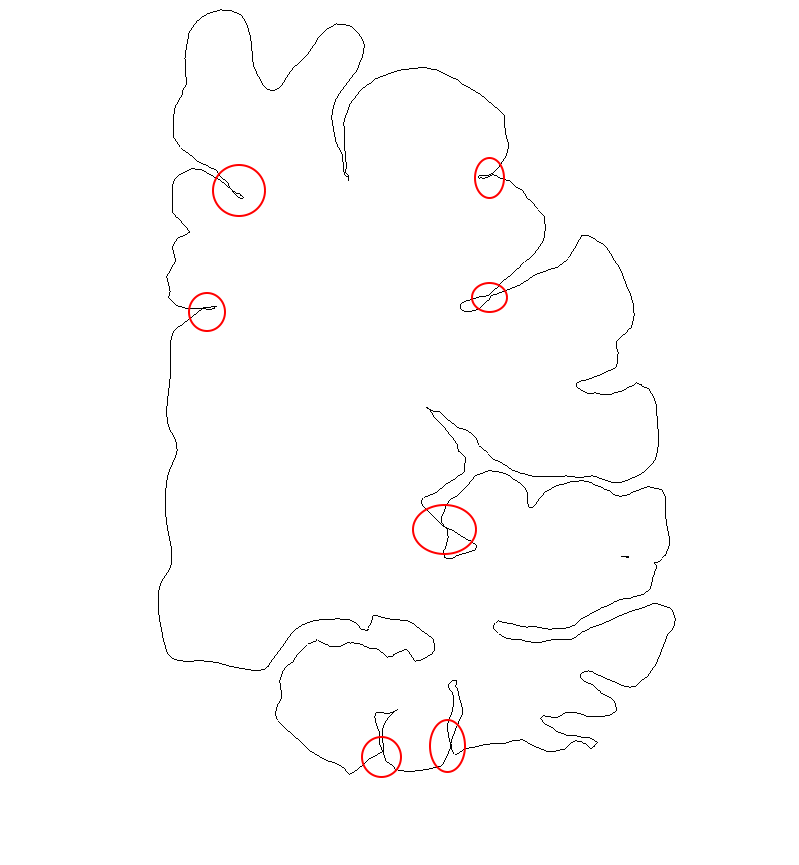
\includegraphics[width=0.5\textwidth]{./graphics/chp3/juncturers-gap.png}
  \caption{Illustration of close junctures in a coronal
    slice of the pial surface created by FreeSurfer.}
  \label{fig:chp3:juncture}
\end{figure}
%
\index{SVM-Tk}
\index{SVM-Tk!\emp{Surface}}
\index{repairing STL surfaces}
%
The following Python snippet illustrates the use of these commands
(included as \emp{mri2fem/chp3/svmtk\_repair\_utilities.py} in the
book scripts):
\newpythonsnippet{chp3}{svmtk_repair_utilities.py}{0}{11}
More commands involving multiple surfaces will be
covered in Chapter \ref{chp:chp4}.

\section{Simulation of diffusion into the brain hemisphere}
\label{sec:chp3:math}

With a mesh representing the domain of interest, we are ready to start
modeling and numerically simulating biophysical processes in this
domain. As a first example, we will study diffusion into the brain
parenchyma of a tracer injected in the subarachnoid space (SAS). This is a
setting encountered, for example, in clinical practice when gadobutrol is 
injected intrathecally (into the cerebrospinal fluid in the spinal
cord SAS)~\cite{ringstad2018brain}, and in experimental
research when fluorescent tracers such as dextran are injected in the
cisterna magna of mice~\cite{iliff2012paravascular,
  xie2013sleep}. Understanding the role of diffusion -- versus other
mechanisms, such as convection -- in the brain parenchyma is a topic of
substantial interest in physiology and medicine~\cite{abbott2018role}.

\subsection{Research question and model formulation}
\label{chp3:model}

Let us ask the following question: assuming that solutes move in the
brain parenchyma by diffusion alone, given an intrathecal injection of
the contrast agent gadobutrol as in glymphatic MRI
investigations~\cite{ringstad2018brain}, what would be the evolution
and distribution patterns of gadobutrol in the brain up to 24 hours
after injection?

To begin addressing this question, we define an initial boundary value
problem for the diffusion of gadobutrol in the brain parenchyma. To do
so, we need to prescribe the computational domain, initial conditions,
parameter values, and boundary conditions for \eqref{eq:diffusion}. It
is often a good idea to also think about the units when defining your
simulation scenario. In brain mechanics at the tissue or organ level,
millimeters (mm) or meters (m) and seconds (s) or minutes (min) are
often suitable choices of units, although we note of course that the
duration of some physiological processes is on the order of days,
months, or years.

Here, we let the concentration $u$ represent the (unit-less)
concentration, of gadobutrol tracer, solving~\eqref{eq:diffusion} in
$\Omega$. The image-based mesh of the left brain hemisphere (for
example \emp{ernie.xdmf}) defines the computational domain
$\Omega$. Formally, $\Omega$ is then the union of the cells in the
mesh. Note that the mesh defines the spatial coordinates of the domain
and consequently the spatial unit. Meshes generated from FreeSurfer
data are typically defined in terms of mm, and thus mm is the default
unit for the spatial scale. The spatial unit can be redefined by
rescaling the mesh, a simple operation in FEniCS. We also
pick a final time and time unit, for instance $T = 1440$ min ($T = 24$
hours).

We assume that no gadobutrol is present in the domain initially,
which translates to the initial condition
\begin{equation}
  \label{eq:chp3:ic}
  u_0(x, 0) = 0 \quad \text{ for all } x \in \Omega.
\end{equation}
Next, we assume that gadobutrol is instantaneously distributed to the brain 
surface via the CSF in the SAS by setting the
boundary condition:
\begin{equation}
  \label{eq:chp3:bc}
  u_d(x, t) = 2.813 \times 10^{-3} \quad x \in \partial \Omega, \quad t > 0
\end{equation}
where $\partial \Omega$ denotes the boundary of $\Omega$, which
represents the pial surface in this scenario. Assuming that the
concentration is known on the pial surface everywhere and at all times
is clearly a simplification. More realistic boundary conditions can
and have been considered in the
literature~\cite{croci2019uncertainty,valnes2020apparent}, and one
could also directly model the movement of tracer in the CSF in the
subarachnoid space~\cite{haga2017numerical,pizzichelli2017numerical}

Brain tissue is heterogeneous and anisotropic, which means that the
effective diffusion coefficient $D$ in~\eqref{eq:diffusion} should vary in
space (and probably in time over longer time scales) and be
tensor valued. We will address these aspects later in this book (in
Chapter~\ref{chap:dti}), but for now we just consider a uniform and
scalar-valued $D$. We estimate the
average effective diffusion coefficient of gadobutrol in brain tissue
to be
\begin{equation}
  D  
  = 4.32 \times 10^{-1} \, \text{mm$^2$/hour}
  = 7.2 \times 10^{-3} \, \text{mm$^2$/min}
\end{equation}
Finally, we assume that there are no sources or sinks of gadobutrol
within the brain parenchyma, and thus set
\begin{equation}
  f(x, t) = 0 \quad x \in \Omega, \quad t > 0.
\end{equation}
Again, this is clearly a simplification that does not account for
potential exit pathways for gadobutrol from the parenchyma.

\subsubsection{Quantities of interest}
The computed solution $u$ will vary in time and space and thus encodes
a substantial amount of information. We are often interested in, first,
merely inspecting the solution visually or qualitatively. For more
quantitative analysis and comparison with experimental or clinical
findings, we typically compute quantities of interest associated with
the solution. These quantities of interest can, for instance, be the
total volume of solute in the entire domain over time:
\begin{equation}
  \label{eq:chp3:qoi}
  Q(t) = \int_{\Omega} u (t) \dx, 
\end{equation}
the average concentration in local regions, or the concentration in
specific points $x$ over time: $u(x, t)$.

\subsection{Numerical solution of the diffusion equation}
\label{sec:chp3:model-problem-numerical-formulation}

%
\index{FEniCS}
%
To compute numerical solutions of the diffusion
equation~\eqref{eq:diffusion} in general, and our specific initial
boundary value problem in particular, we will use a finite difference
discretization in time and a finite element discretization in
space~\cite{langtangen2019introduction,
  gockenbach2006understanding}. This is a common approach and we will
implement this numerical scheme using FEniCS Project
software~\cite{logg2012automated,alnaes2015fenics,langtangen2016solving}. As
mentioned in our introductory remarks, we strongly encourage readers
unfamiliar with numerically solving partial differential equations
(PDEs) or FEniCS to study the FEniCS
tutorial~\cite{langtangen2016solving} before proceeding.

For the discretization in time, we define a set of discrete times $0 =
t_0 \leq t_1 \dots \leq t_N = T$, where $N$ is the number of time
steps and the time step (size) is $\tau_n = t_n - t_{n-1}$ for $n = 1,
\dots, N$. Our aim is to compute approximate solutions $u^n_h$
of~\eqref{eq:diffusion} such that $u^n_h \approx u(t_n)$ for each
$n$. To this end, we introduce the (first-order, backward) finite
difference approximation in time
\begin{equation}
  u(t_n) \approx u^n, \quad
  u_t(t_n) \approx \frac{1}{\tau_n} (u^n - u^{n-1}),
\end{equation}
and obtain the time-discrete equations for $n = 1, \dots, N$:
\begin{equation}
  \label{eq:chp3:time-discrete}
  \frac{1}{\tau_n} (u^n - u^{n-1}) - \Div D \Grad u^n = f(t_n) \quad \text{in } \Omega. 
\end{equation}

Next, for the finite element discretization in space, we derive a
discrete variational formulation of~\eqref{eq:chp3:time-discrete} by
multiplying it by test functions $\phi$ belonging to a finite element space $V$
defined relative to the mesh $\mesh$, integrating by parts, and moving
all known terms to the right-hand side to obtain the following fully
discrete problem: find the discrete solution $u_h^n \in V$ at each
time $n = 1, \dots, N$ such that
\begin{equation}
  \label{eq:chp3:discrete}
  \inner{u_h^n}{\phi} + \tau_n \inner{\Grad u_h^n}{\Grad \phi}
  =  \inner{u_h^{n-1}}{\phi} + \tau_n \inner{f^n}{\phi},  
\end{equation}
for all test functions $\phi \in V$, where we use the
$L^2(\Omega)$-inner product notation
\begin{equation}
  \inner{u}{\phi} = \int_{\Omega} u \, \phi \dx.
\end{equation}
In addition, we require the discrete solution to satisfy the
boundary condition~\eqref{eq:chp3:bc}, and to initially be given by the
initial condition~\eqref{eq:chp3:ic}.   

The fully discrete equation~\eqref{eq:chp3:discrete} is a good
starting point for the FEniCS implementation of this scheme. We choose
to approximate the solution using continuous piecewise linear finite
element spaces. 

\subsection{Implementation using {\fenics}}
\label{sec:chp3:fenics-code-implementation}

Our model problem is very similar to the heat equation problem
presented in the FEniCS tutorial~\cite[Chapter
  3.1]{langtangen2016solving}, and we base our implementation on the
algorithm and code presented there. We begin by importing the Python
module \pythoninline{fenics}, and we also import \pythoninline{numpy}
as a handy Python module for general numerics:
\newpythonsnippet{chp3}{diffusion.py}{0}{2}
%
\index{file format!XDMF}
\index{file format!h5}
%
\noindent We then read the mesh that we have just generated into the FEniCS
program. We use the XDMF mesh format and reader, since they are suitable for
large scale simulations and work seamlessly with MPI-parallel computing:
\newpythonsnippet{chp3}{diffusion.py}{4}{13}

\noindent We now define the parameters for the time discretization. We
choose to simulate up to 72 hours and choose a time step $\tau$
(\pythoninline{tau}) of three min. Note that we use the Constant type to
represent \pythoninline{time}; it is useful for updating functions
depending on time later. In addition, keeping track of the parameter units
used is good practice. Here we just use the comments, although much more
rigorous solutions, such as SymPy's unit
systems~\cite{meurer2017sympy}, could be used.
\newpythonsnippet{chp3}{diffusion.py}{15}{18}

\noindent We also define the diffusion coefficient, source function
and initial condition (even though the latter two are just zero):
\newpythonsnippet{chp3}{diffusion.py}{20}{25}

We now move on to consider the specification of the finite element
discretization. We first define the finite element space $V$ as the
Lagrange elements of degree 1 defined relative to our mesh, and then
define a \pythoninline{TrialFunction} and \pythoninline{TestFunction}
over this space 
\newpythonsnippet{chp3}{diffusion.py}{27}{30}

\noindent We next define a \pythoninline{Function} to hold the value
of the solution at the previous time step \pythoninline{u_}, and
initialize this function with the initial condition \pythoninline{u0}:
\newpythonsnippet{chp3}{diffusion.py}{32}{35}

\noindent Having defined these objects, we can express the variational
problem~\eqref{eq:chp3:discrete}, to be solved at each time step, in
code. We also redefine \pythoninline{u} as a
\pythoninline{Function} to represent the solution at the current time:
\newpythonsnippet{chp3}{diffusion.py}{37}{42}

\noindent Having defined the finite element space, we can also define
the boundary condition, which will be imposed on the linear system of
equations at each time step. 
\newpythonsnippet{chp3}{diffusion.py}{47}{51}
\noindent Note how we let the boundary value
\pythoninline{u_d} depend on the previously defined
\pythoninline{Constant} \pythoninline{time}. This way, when
\pythoninline{time} updates, so will \pythoninline{u_d} and
\pythoninline{bc}.

We have now defined all the elements of the model problem and
numerical method and can start stepping through the solution
algorithm. Since the bilinear form on the left hand side
of~\eqref{eq:chp3:discrete} does not vary in time, we can assemble
this matrix once, outside the time loop, for the sake of efficiency:  
\newpythonsnippet{chp3}{diffusion.py}{53}{55}
%
\index{ParaView}
%
In order to view our solutions using ParaView, we define a PVD file 
(indicated by the suffix \pythoninline{.pvd}) for 
%We define a PVD file (indicated by the suffix \pythoninline{.pvd}) for
storing the solution, computed at each time step, as well as the initial data. 
%in VTK format and
%store the initial solution. 
\newpythonsnippet{chp3}{diffusion.py}{57}{60}
\noindent %This is a file format convenient for visualization in
%ParaView. 
%Note that it is not a convenient format for reading the
%functions back into FEniCS however; for this purpose one should
%instead use the XDMF or h5 formats.
The PVD format is nice for visualization in ParaView but is not a convenient 
format for reading the functions back into FEniCS; for this purpose one should
instead use the XDMF or h5 formats.

Next, we compute the number of time steps, \pythoninline{N}, and initialize
NumPy arrays for storing computational quantities of interest at each
time step, such as the total amount of solute (\pythoninline{amounts})
cf.~\eqref{eq:chp3:qoi}, and the concentration (\pythoninline{concs})
at a specific point (\pythoninline{p}).
\newpythonsnippet{chp3}{diffusion.py}{62}{68}

Now we are ready to start stepping through time and to solve the finite
element system at each time step. We increment
\pythoninline{time} with the timestep~\pythoninline{tau}, assemble
the right hand side into the vector \pythoninline{b}, apply the
Dirichlet boundary condition, solve the resulting linear system using
an iterative solver (gmres, amg), and update the previous solution
with the current solution:
\newpythonsnippet{chp3}{diffusion.py}{70}{85} %
Note that the use of `gmres', in the solve function above, tells {\fenics} to 
use the `Generalized Minimal Residual Method' as the iterative solution 
technique; the use of `amg' specifies that the `Algebraic Multigrid Method' 
should be used as the preconditioning approach for the iterative method.  The 
interested reader can find more on the GMRES method, including convergence 
details, in \cite{greenbaum1997} while a review of algebraic multigrid 
is also available \cite{stuben2001}.  Both GMRES and AMG are well-suited to 
parabolic problems, like \eqref{eq:diffusion}, and {\fenics} supports several 
alternative iterative methods and preconditioning options 
\cite{langtangen2016solving} that can investigated if desired.  % 


We can compute the total amount of solute by integrating the concentration
over the domain, and the concentration in the specified point by
evaluating the computed solution at this point. We also store the
entire solution to the PVD file. Writing the solution to file can take
some time, and, for fine time steps, it may often be practical to 
do this only say every second, or 10th or 100th time step:
\newpythonsnippet{chp3}{diffusion.py}{87}{96}
It can also be practical to store the computed quantities in a file; reading 
the contents of the file, for plotting, at a later time:
\newpythonsnippet{chp3}{diffusion.py}{98}{101}

\index{plotting!matplotlib}
The Python module matplotlib offers quick and convenient plotting, and
we use this module to plot the quantities of interest (the total
amount of solute and the concentration at the given point) over time
and save these in, for instance, PNG format. The resulting plots are
shown in Figure~\ref{fig:chp3:png-plots}. The complete script
(including the plot code) is available in the book scripts
(\emp{mri2fem/chp3/diffusion.py}).  The concentration at various points can be 
investigated by modifying the value of $p$, in the script, as shown in the code 
block below:
\newpythonsnippet{chp3}{diffusion.py}{62}{68}

\begin{figure}
    \begin{tabular}{cc}
    \imagetop{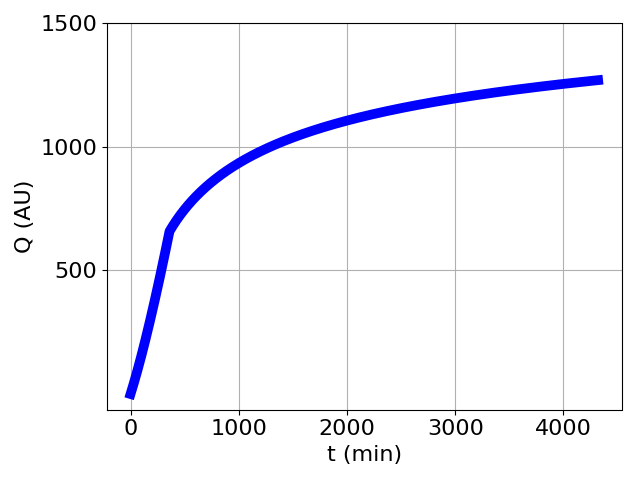
\includegraphics[width=0.49\textwidth]{./graphics/chp3/amounts.png}} &
    \imagetop{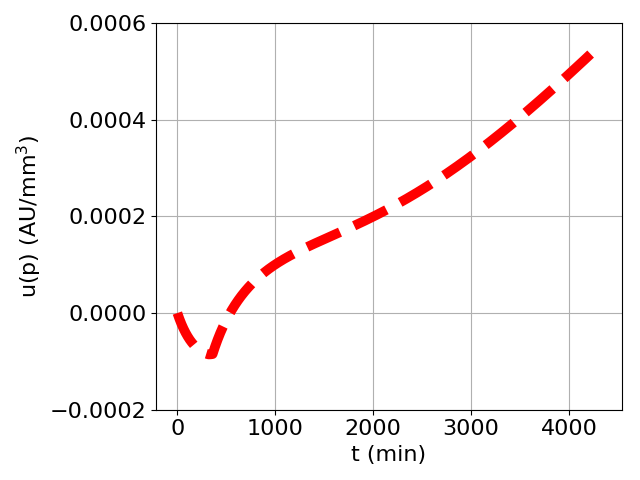
\includegraphics[width=0.49\textwidth]{./graphics/chp3/concentrations.png}}
    \end{tabular}
    \caption{Plots of the quantities of interest, in arbitrary units (AU), 
	associated with the computed concentration: total amount of solute 
	$Q$ over time $t$ (left) and concentration $u(p, t)$ for a given 
	point $p$ over time $t$ (right).}
    \label{fig:chp3:png-plots}
\end{figure}

\index{mass lumping}
The approximation of the solute concentration at a given point over
time demonstrates an interesting numerical artefact: the concentration
drops below zero to become negative at early times (between 0 and 550
min). Negative solute concentrations are clearly unphysiological, but
a common numerical problem with diffusion simulations. A partial and
often used remedy, including within the context of diffusion simulations
in the brain~\cite{croci2019uncertainty}, is \emph{mass lumping}. Mass
lumping can reduce spurious negative concentrations, but may worsen
the overall convergence of the numerical solutions. We will return
to this aspect in Chapter~\ref{chp:chp6}.

\subsection{Visualization of solution fields}
\index{ParaView}
To visualize computed solution fields, for instance, the
concentrations stored in u.pvd (and the associated u*.vtu files) in
the previous section, we will use ParaView. After launching the
ParaView graphical user interface (see
Chapter~\ref{sec:chp2:paraview}), we can open collections of files
by \button{File$\rightarrow$Open} and selecting the .pvd or .vtu
file(s) from the folder results. ParaView is a powerful and versatile 
visualization tool, and we refer the reader to the extensive resources 
available on the ParaView website~\cite{paraview:web} for guides, tutorials, 
and so forth. In Figure~\ref{fig:chp3:approximate-numerical-soln} below, we 
used ParaView to plot clips of snapshots of the solute
concentrations, with the x-axis as the normal direction for the clips
and the view direction, rescaled to the data range over all
  timesteps, and using the viridis color scheme.
\begin{figure}[h]
    \begin{tabular}{l l l l}
    \imagetop{2h}&  \imagetop{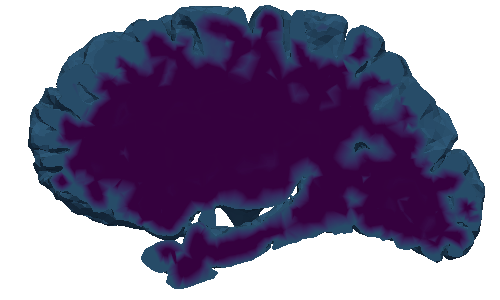
\includegraphics[width=0.4\textwidth]{./graphics/chp3/mri-tracer/2h}}&
    \imagetop{6h}&  \imagetop{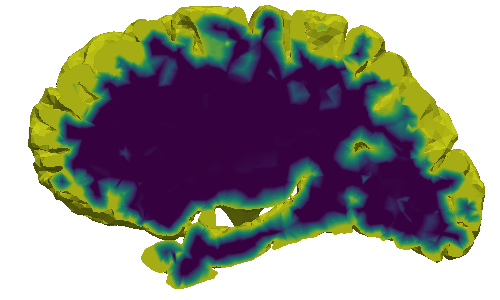
\includegraphics[width=0.4\textwidth]{./graphics/chp3/mri-tracer/6h}}\\
    \imagetop{12h}& \imagetop{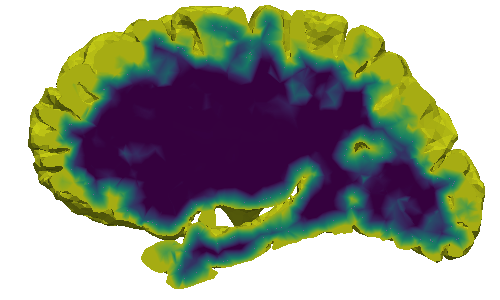
\includegraphics[width=0.4\textwidth]{./graphics/chp3/mri-tracer/12h}}&
    \imagetop{24h}& \imagetop{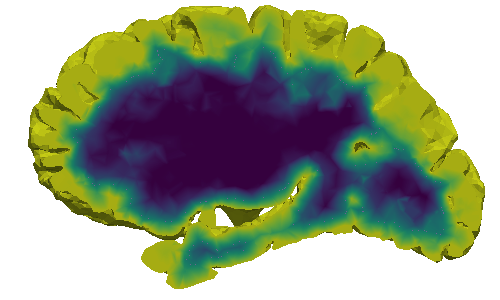
\includegraphics[width=0.4\textwidth]{./graphics/chp3/mri-tracer/24h}}\\
    \imagetop{48h}& \imagetop{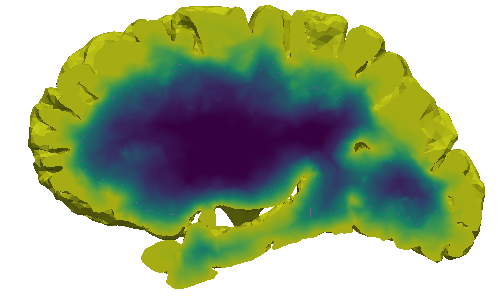
\includegraphics[width=0.4\textwidth]{./graphics/chp3/mri-tracer/48h}}&
    \imagetop{72h}& \imagetop{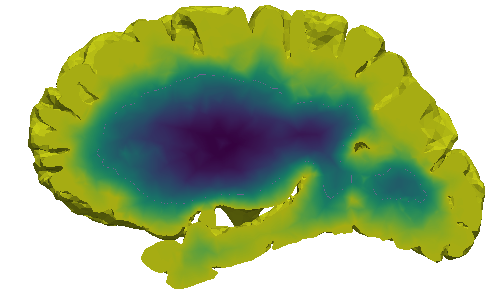
\includegraphics[width=0.4\textwidth]{./graphics/chp3/mri-tracer/72h}}
    \end{tabular}
    \caption{Simulated tracer concentration at given times (2, 6, 12, 24, 48, 
	and 72 hours) post-injection into subarachnoid CSF. Blue 
	represents lower values, while yellow represents higher values.  
	The scalar concentration is plotted on the whole brain volume mesh; the 
	mesh has been sliced, in ParaView, for sagittal visualization.}
    \label{fig:chp3:approximate-numerical-soln}
\end{figure}

\section{Advanced topics for working with larger cohorts}
\label{sec:chp3:advanced}
\index{DICOM}
We have now covered the entire computational pipeline from MR images
to numerical simulation and visualization for a single imaging
modality, a single stack of MRI data, and a single simulation scenario. In
this section, we will cover some more advanced topics useful for
working with more complex DICOM data collections.

\subsection{Scripting the extraction of MRI series}

When processing larger DICOM datasets consisting of a large number of
patients and/or studies, the extraction of single MRI series via a
graphical interface can become tedious and error-prone. An alternative
approach is to script the extraction of specific MRI series using
FreeSurfer command line utilities.

%
\index{FreeSurfer!\emp{mri\_probedicom}}
%
The extraction process consists of two command line steps: probing the
dataset for a given tag name and then extracting all data with the
given tag from the database. We will utilize the FreeSurfer command
\emp{mri\_probedicom} to examine and probe the DICOM metadata, so
ensure that FreeSurfer is installed and configured (see
Chapter~\ref{sec:chp2:tools:freesurfer}) before proceeding. The useful
command \emp{mri\_probedicom} can be used to compare the meta
data of different DICOM files with the flag \emp{-{}-compare} followed
by two DICOM filenames. We can also view individual images associated to 
a particular DICOM file collection by specifying the image name and using 
the flag \emp{-{}-view}, for example:
\terminal{\$ cd \erniedicom/DICOM \\
\$ mri\_probedicom -{}-i IM\_0162 -{}-view
}

\noindent Alternatively, we may desire to look for a specific tag.  DICOM stores 
tags as numeric identifiers.  If we know that our MR scanner saves the 
\textit{Protocol Name} to tag 18 1030, as in the book DICOM data set, then we 
could probe the DICOM data for tag 18 1030 with the command:
%
%\noindent To probe the book DICOM data set for the tag \textit{Protocol Name}, which
%is associated with the numeric identifier 18 1030, issue the command
\terminal{\$ mri\_probedicom -{}-i IM\_0162 -{}-t 18 1030 \\
T13D
} 
\noindent The complete description of possible options to
\emp{mri\_probedicom} can be viewed by using the \emp{-{}-help} flag.

To extract files with a specific tag on the command-line, we can thus
probe each file, and copy files with a specific tag to a new
directory. This can be accomplished via, for example, the following bash script
(also available at \emp{mri2fem/chp3/mri\_sort.sh}). The script
takes three types of input, namely, the DICOM directory, the output directory and
an identifier for the protocol name:
\begin{lstlisting}[style=bashStyle]
#!/bin/bash
# 1st argument $1: input DICOM folder
# 2nd argument $2: the output copy directory
# 3rd argument $3: the identifier 

# Find all files in the directory and subdirectories
files=$(find $1 -type f ) 
for j in ${files}; do
    # Probe for protocol name (18 1030)
    name=$(mri_probedicom --i ${j} --t 18 1030) 

    # Check if identifier is part of protocol name.
    if [ "${name/$3}" != "$name" ]
       then
       # Copy file to (new) subdirectory 
       mkdir -p ${2}/${name//[[:blank:]]/}  
       cp ${j}  ${2}/${name//[[:blank:]]/} 
    fi
done
\end{lstlisting}

This script uses the bash command \emp{find} and the flag \emp{-type
  f} to find all files in the input directory and its
subdirectories. The script will go through all the files and probe
each file for the protocol name and check if the protocol name
contains the identifier argument. Each file with the identifier in the
protocol name will be copied to a folder named by the protocol name in
the output directory. Spaces are removed from the protocol name, which is preferred to avoid errors when using FreeSurfer.
Thus, we can use the script to extract all the images with the \emp{T1}
string in the protocol name from the sample data set:
\terminal{\$ cd \erniedicom \\
\$ ./mri\_sort.sh ./DICOM ./ "T1" }

\subsection{More about FreeSurfer's \emp{recon-all}}
\label{sec:chp3:advanced:recon-all}
%
\index{FreeSurfer!\emp{recon-all}}
%
The command \emp{recon-all} is the primary command for FreeSurfer,
since it will start the segmentation process. We have already
described the necessary flags for this command, but we will continue
the description with additional options. This description will be
on an introductory level. However, the interested reader can use the
flag \emp{-help}, which will print detailed information about the
entire process and provide references to related articles and texts.

The command \emp{recon-all} is a sequential process that consist of 34
different stages, divided into three different
steps~\cite{freesurfer-wiki}. Data will be produced throughout the
process, and are often required as input for the next stage.  The recon-all 
command can be used to execute the full set of 34 stages or to execute only 
a portion of the stages.  Some of the available \emp{recon-all} flags are 
shown below; a full list of options is available 
online\footnote{see \url{https://surfer.nmr.mgh.harvard.edu/fswiki/recon-all/}}. 
%We can
%initiate each step separately by using the following flags instead of
%\emp{-all}.
% changed the autorecon-1 to autorecon1, etc in line with the freesurfer 
% documentation from https://surfer.nmr.mgh.harvard.edu/fswiki/recon-all
\begin{itemize}
\item \emp{recon-all -autorecon1 -subjid \textit{subject}}: starts the step-1 process, which includes stages 1 to 5, involving normalization and skull stripping using the data in the subject folder named \textit{subject}; 
\item \emp{recon-all -autorecon2 -subjid \textit{subject}}: starts the step-2 process, which includes stages 6 to 23, involving segmentation and surface generation using the data in the subject folder named \textit{subject};
\item \emp{recon-all -autorecon3 -subjid \textit{subject}}: starts the step-3 process, which includes stages 24 to 34, involving statistical data generation and final parcellation using the data in the subject folder named \textit{subject};
%\item \emp{recon-all -autorecon-pial -subjid \textit{subject}}: starts the construction of the surfaces, which include stages 16 to 23, involving various surface operations using the data in the subject folder named \textit{subject}; 
%\item \emp{-autorecon-all}: equivalent to \emp{-all}. 
\end{itemize} 

These flags can be useful for restarting the segmentation. For
instance, if a failure occurred at stage 34, then we can start over
from stage 24 rather than from the beginning by using the flag
\emp{-autorecon3}, as shown above. This approach can also be useful when it is
necessary to rerun the segmentation process after correcting an
error. In FreeSurfer, there exist two types of errors, known as hard
and soft errors. Hard errors will terminate the segmentation process,
while soft errors are errors that we find in the produced data. Soft
errors are mostly segmentation errors, such as the inclusion of the
dura in the segmentation and erroneous segmentation of white
matter. In such a case, we could edit the segmentation to correct the error, 
and run \emp{recon-all} with the flag \emp{-autorecon2-pial}.  Specific details 
for the \emp{-autorecon2-pial} flag, which we do not discuss here, can be found 
in the FreeSufer documentation \cite{freesurfer-wiki}.  This will create new 
surfaces based on the corrected segmentation files. The correction of soft 
errors will not be covered further in this book. Instead, we refer to the 
FreeSurfer documentation~\cite{freesurfer-wiki}.

%
\index{FreeSurfer}
\index{MRI!T2}
%
We continue with the flag \emp{-sd}, which can be used to specify the
subject directory for the \emp{recon-all} command. This can be quite
useful for separating the segmentation data for different
cohorts. The segmentation of CSF filled structures, such as the
ventricular system, may require the additional use of T2-weighted MR
images to obtain an acceptable quality. We can include T2 MR images with the
flag \emp{-T2}, and we can use the flag \emp{-T2-pial} to use
the T2 MRI in the construction of pial surfaces.

The segmentation in FreeSurfer is based on the segmentation atlas of
healthy subjects; therefore, the segmentation can often encounter hard
errors for patients with abnormal brain anatomy. We can often allow
the segmentation to finish if we add the flag \emp{-notalairach},
which causes \emp{recon-all} to skip assertion points in the first step. The
log of \emp{recon-all} is documented in the folder \emp{scripts}
and all the specific command lines can be found in \emp{touch}.




\chapter{Introducing heterogeneities}
\label{chp:chp4}

In this chapter, we will consider how to mark, remove, and mesh
different regions of the brain and its environment based on
{\freesurfer} segmentations. We will
\begin{itemize}
\item
  Create hemisphere meshes differentiating between gray and white matter,
\item
  Create hemisphere meshes without ventricles,
\item
  Create brain meshes by combining the two hemispheres,
\item
  Map parcellations\footnote{A parcellation is a way of dividing the brain 
  into distinct regions. {\freesurfer}, for instance, does this as part of 
  the \emp{recon-all} process and this is why we can use Freeview to view the 
  different parts of a subject's brain, such as the hippocampus or anterior 
  cingulate, after \emp{recon-all} completes.} 
  onto brain meshes, and
\item
  Locally refine parcellated brain meshes.
\end{itemize}

\section{Hemisphere meshing with gray and white matter}
\label{sec:chp4:tools:gray-white}

Gray and white matter differ substantially in their
characteristics. These differences can often be represented in
mathematical models and simulations by differing material
properties. For instance, denoting the domains occupied by gray and
white matter by $\Omega_g$ and $\Omega_w$ respectively, we may want to
consider heterogeneous diffusion tensors in~\eqref{eq:diffusion}, for
example, such that
\begin{equation}
  \label{eq:K}
  D = D(x) = \left \{
    \begin{matrix}
      D_g & \quad x \in \Omega_g, \\
      D_w & \quad x \in \Omega_w 
    \end{matrix}
    \right .
\end{equation}
where $D_g$ and $D_w$ take on different values, and $D_g$ may be
scalar-valued and $D_w$ tensor-valued. To represent fields such as $D$
in numerical simulations, it is useful to transfer the information
about gray and white matter from the magnetic resonance (MR) images
into the meshes. To introduce the basic concepts of differentiating
brain regions, we will once more create a computational mesh of the left
hemisphere.  In Chapter~\ref{chp:chp3}, all of the mesh tetrahedrons belonged 
to a single region.  In this chapter, we extend the previous approach 
by creating a mesh where the individual tetrahedrons will be labeled as 
belonging to the gray matter, the white matter, or the ventricles. In short, 
we will
\begin{itemize}
\item
  Create STL files from the pial and white FreeSurfer left hemisphere
  surfaces, 
\item
  Create a mesh from these STL files conforming to the interior interfaces
  between white and gray matter, using \svmtk{}, and
\item
  Include tags for different regions of the mesh.  That is, for each 
  tetrahedron in the mesh we want to label it as residing in the 
  `gray matter', `white matter', `ventricles', etc.     
\end{itemize}

\subsection{Converting pial and gray/white surface files to STL}
\index{FreeSurfer}
\index{FreeSurfer!\emp{mris\_convert}}
Starting with the \freesurfer{} segmentation and using the book data
from \emp{freesurfer/ernie/surf/} as an example, we first convert the
left hemisphere pial surface (\emp{lh.pial}) and gray-white interface
surface (\emp{lh.white}) files to the STL format (as described in
Chapter~\ref{sec:chp3:surfaces}):
\terminal{\$ mris\_convert ./lh.pial pial.stl\\
\$ mris\_convert ./lh.white white.stl
}
\noindent We can now also improve the quality of the resulting
surfaces as discussed in
Chapter~\ref{sec:chp3:improved-volume-meshing}\footnote{We leave the
  precise code for this as an exercise for the reader. The resulting
  files could be called \emp{lh.pial.smooth.stl} and
  \emp{lh.white.smooth.stl}, respectively. For simplicity, we assume that the
  resulting pial and white surface STL files are (re)named
  \emp{lh.pial.stl} and \emp{lh.white.stl}, respectively, in the following. As 
  noted in Chapter~\ref{chp:chp3}, the automatic addition of the prefix lh., in
  lh.pial.stl, can be avoided by using ./ in the output filename.}.

\subsection{Creating the gray and white matter mesh}%
\label{sec:chp4:tools:gray-white:mesh-creation}
\index{SVM-Tk!\emp{Domain}}
\index{SVM-Tk!\emp{SubdomainMap}}
\index{ParaView}
Given these two surfaces, we can create a volume mesh conforming to
the interior (gray--white) surface, with the white and gray regions
identified separately. We will use \svmtk{} for this task, and
proceed with an \svmtk{} code example. We will wrap the main
functionality in a Python function
\pythoninline{create\_gw\_mesh}. This function can then, for instance,
be called as
\newpythonsnippet{chp4}{two-domain-tagged.py}{25}{28}
to use the two STL surface files from above as input and create a new
file \emp{ernie-gw.mesh} for the resulting volume mesh.

Our function first loads the two surfaces using \svmtk{}:
\newpythonsnippet{chp4}{two-domain-tagged.py}{0}{8}

\noindent Notice that the list \pythoninline{surfaces = [pial, white]} contains 
two surfaces; the order of these surfaces in this list will matter.  We next 
create a tailored \svmtk{} \pythoninline{SubdomainMap} object that represents 
a map between regions defined by surfaces and tags. This map is defined by
(repeated) calls to \emp{smap.add} with a string representing the
region and an integer representing the tag as arguments. The (binary)
string is a sequence of zeros and ones, with zero denoting the outside
and one the inside\footnote{Note that the STL surface 
format includes information about the orientation of the surfaces via the 
surface normals: each surface thus has an orientation, with an inside and an 
outside direction.}.
\newpythonsnippet{chp4}{two-domain-tagged.py}{9}{14}

Intuitively, \pythoninline{smap.add("10",1)} will mean `those tetrahedron 
inside surface 1 (pial surface) and outside surface 2 (white matter surface) 
should be marked with the numeric (tag) value of 1' while 
\pythoninline{smap.add("11",2)} will mean `those tetrahedron inside surface 1 
(pial surface) and inside surface 2 (white matter surface) should be marked 
with the numeric (tag) value of 2'.  At this point, however, \svmtk{} does not 
know that the \pythoninline{surfaces} list and our 
\pythoninline{SubdomainMap} object, \pythoninline{smap}, are related.  Relating 
a surface list to a \pythoninline{SubdomainMap} object is handled by creating 
a \pythoninline{Domain} object; a \pythoninline{Domain} object is constructed  
from the ordered list of surfaces and the subdomain map as follows:
%
%An \svmtk{} \pythoninline{Domain} object can be constructed from the
%ordered list of surfaces and the subdomain map:
%
\newpythonsnippet{chp4}{two-domain-tagged.py}{16}{19}

%\noindent Note that the \pythoninline{Domain} object here links the
%surfaces and the subdomain map. 
\noindent The \pythoninline{Domain} object reads the entries, registered above 
as \pythoninline{smap.add("10",1)} etc, of the 
\pythoninline{SubdomainMap} with respect to the ordering of the entries in 
our \pythoninline{surfaces} list.  The important point here is that the 
order of the entries in the \pythoninline{surfaces} list plays a key role; 
permuting the entries will yield different results.  % 
%The order of the entries in the list
%of surfaces is matched to the binary region strings in the subdomain
%map. 
For the code above, the string \pythoninline{"10"} %referring to the list \pythoninline{[pial, white]} 
is interpreted as `inside pial' and `outside white' and thus represents all 
tetrahedron in the region between the pial and white surface; this region 
consists of only the gray matter. Similarly, the string \pythoninline{"11"} is 
interpreted as 'inside pial' and 'inside white' and thus represents all 
tetrahedron in the white matter region since this region lies within both 
surfaces.  %
%
%region inside the gray--white surface, that
%is, the white matter. 
We will discuss \pythoninline{SubdomainMap} further in 
Chapter~\ref{chp4:subdomains} below.

With \pythoninline{domain}, we can now create a volume mesh of
suitable resolution and save it in the .mesh format (as in
Chapter~\ref{subsec:chp3:mesh-creation}):
\newpythonsnippet{chp4}{two-domain-tagged.py}{20}{24}
This script is also available as \emp{mri2fem/chp4/two-domain-tagged.py} in the
book scripts, and can be run from there as:
\terminal{\$ python two-domain-tagged.py}
\index{meshio!\emp{meshio-convert}}
\noindent As before, the resulting \emp{.mesh} file can be converted to different formats
using meshio. For instance, to convert to the ParaView-friendly .vtu format, use:
\terminal{\$ meshio-convert ernie-gw.mesh ernie-gw.vtu}

We used ParaView to visualize the tags associated with this mesh
in Figure~\ref{fig:chp4:ernie-tagged-twodomain-mesh}.  To see a view similar 
to that of Figure~\ref{fig:chp4:ernie-tagged-twodomain-mesh} in ParaView, first 
load \emp{ernie-gw.vtu} by selecting \button{File$\rightarrow$Open} and s
electing \emp{ernie-gw.vtu}, then click \button{Apply} to show the mesh.  In 
the left-hand window, under the \emp{Coloring} heading, select the second 
entry titled \emp{medit:ref}.  Now select 
\button{Filters$\rightarrow$Alphabetical$\rightarrow$Clip} from the top menu 
bar.  The clipping plane should, by default, appear in the middle of the mesh 
with the (red) clipping plane in the sagittal orientation.  Click the 
\button{Apply} button in the left-hand window to cut the mesh and reveal the 
tagged gray and white matter (tagged) tetrahedron.  We see that the
mesh cells associated with the gray matter region have the value 1,
while the cells associated with the white matter region have the value
2, as defined by our subdomain map.

\begin{figure}
  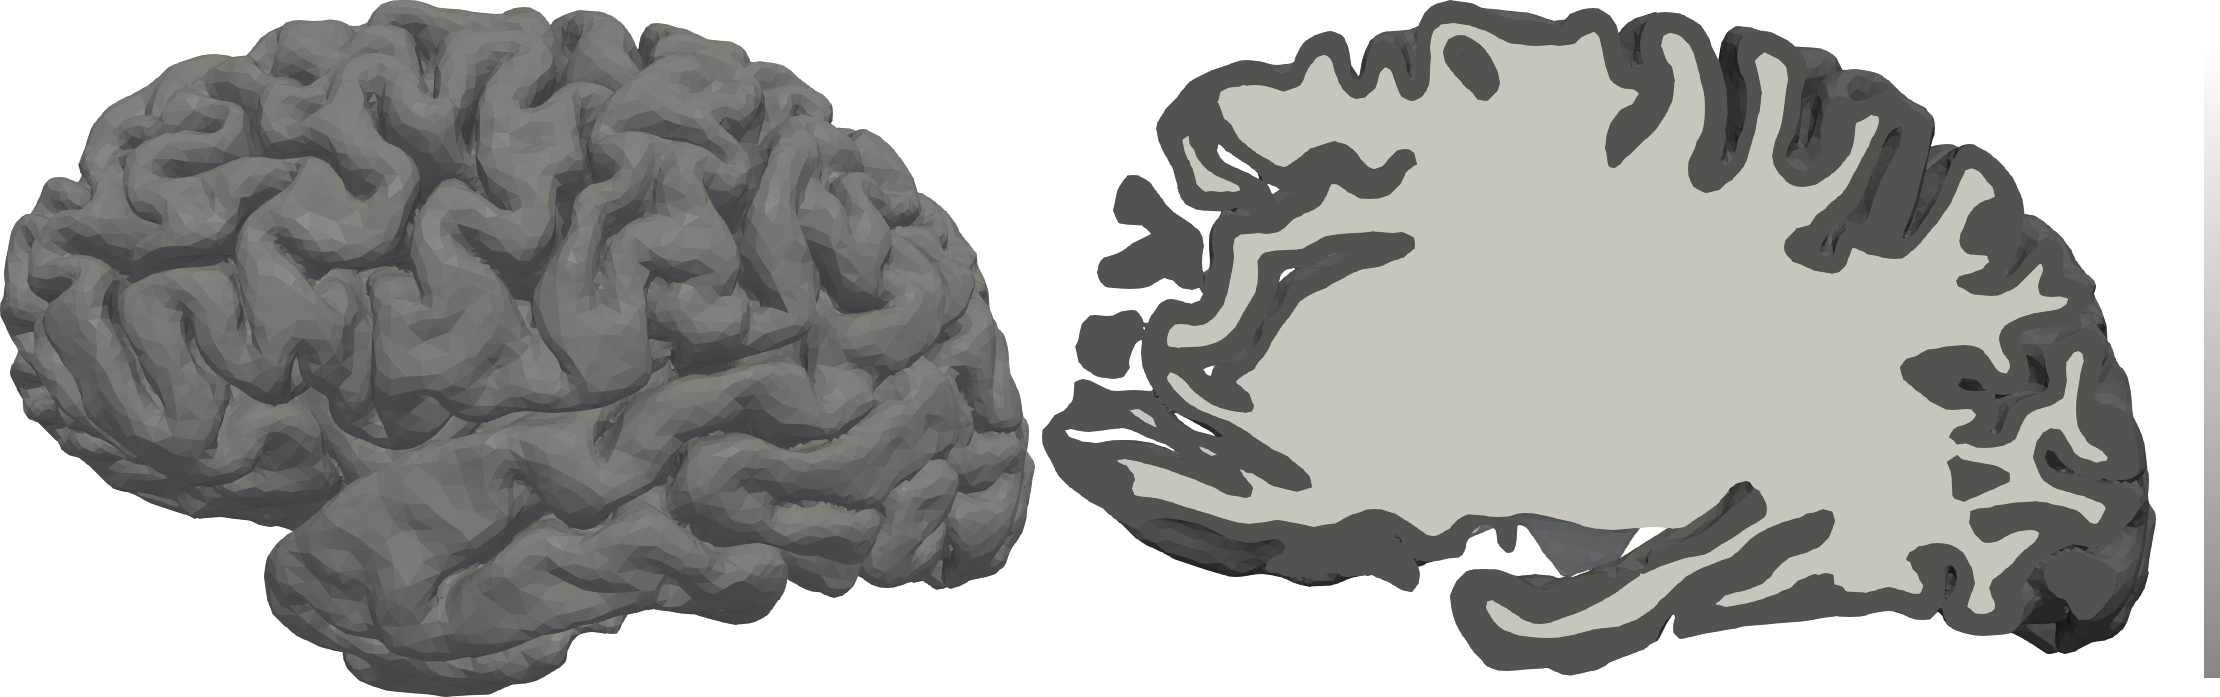
\includegraphics[width=0.99\textwidth]{./graphics/chp4/two-domain-tagged-bw.png}
  \caption{Volume mesh of the left hemisphere conforming to the
    interior gray--white interface.  Gray matter is tagged with a value of 1 
    and white matter is tagged with a value of 2.  The color scale is inverted. 
    A sagittal view (left) of the left hemisphere volume mesh and a sliced 
    (right) view exposes the interior white matter region.}
  \label{fig:chp4:ernie-tagged-twodomain-mesh}
\end{figure}

As a side note, we observe that the ventricles have been labeled as
white matter (see Figure \ref{fig:chp4:ernie-tagged-twodomain-mesh},
right), since the ventricles are positioned inside the gray--white
interface surface. Removal of the ventricles from our computational mesh
is the topic of Chapter~\ref{sec:chp4:tools:remove-vent}.

\subsection{More about defining \svmtk{} subdomain maps}  
\label{chp4:subdomains}
\index{SVM-Tk!\emp{SubdomainMap}}
To provide more detail about the \svmtk{} feature
\pythoninline{SubdomainMap}, we consider another, more involved
example. We now assume that we have four surfaces: a left pial
surface, a right pial surface, the whole white matter surface and a
surface enclosing the ventricles. A schematic of this set-up is
illustrated in Figure~\ref{fig:chp4:smap-example}. Now, let us see how
we can tag all the tetrahedra of the ventricles.
\begin{figure}[t]
  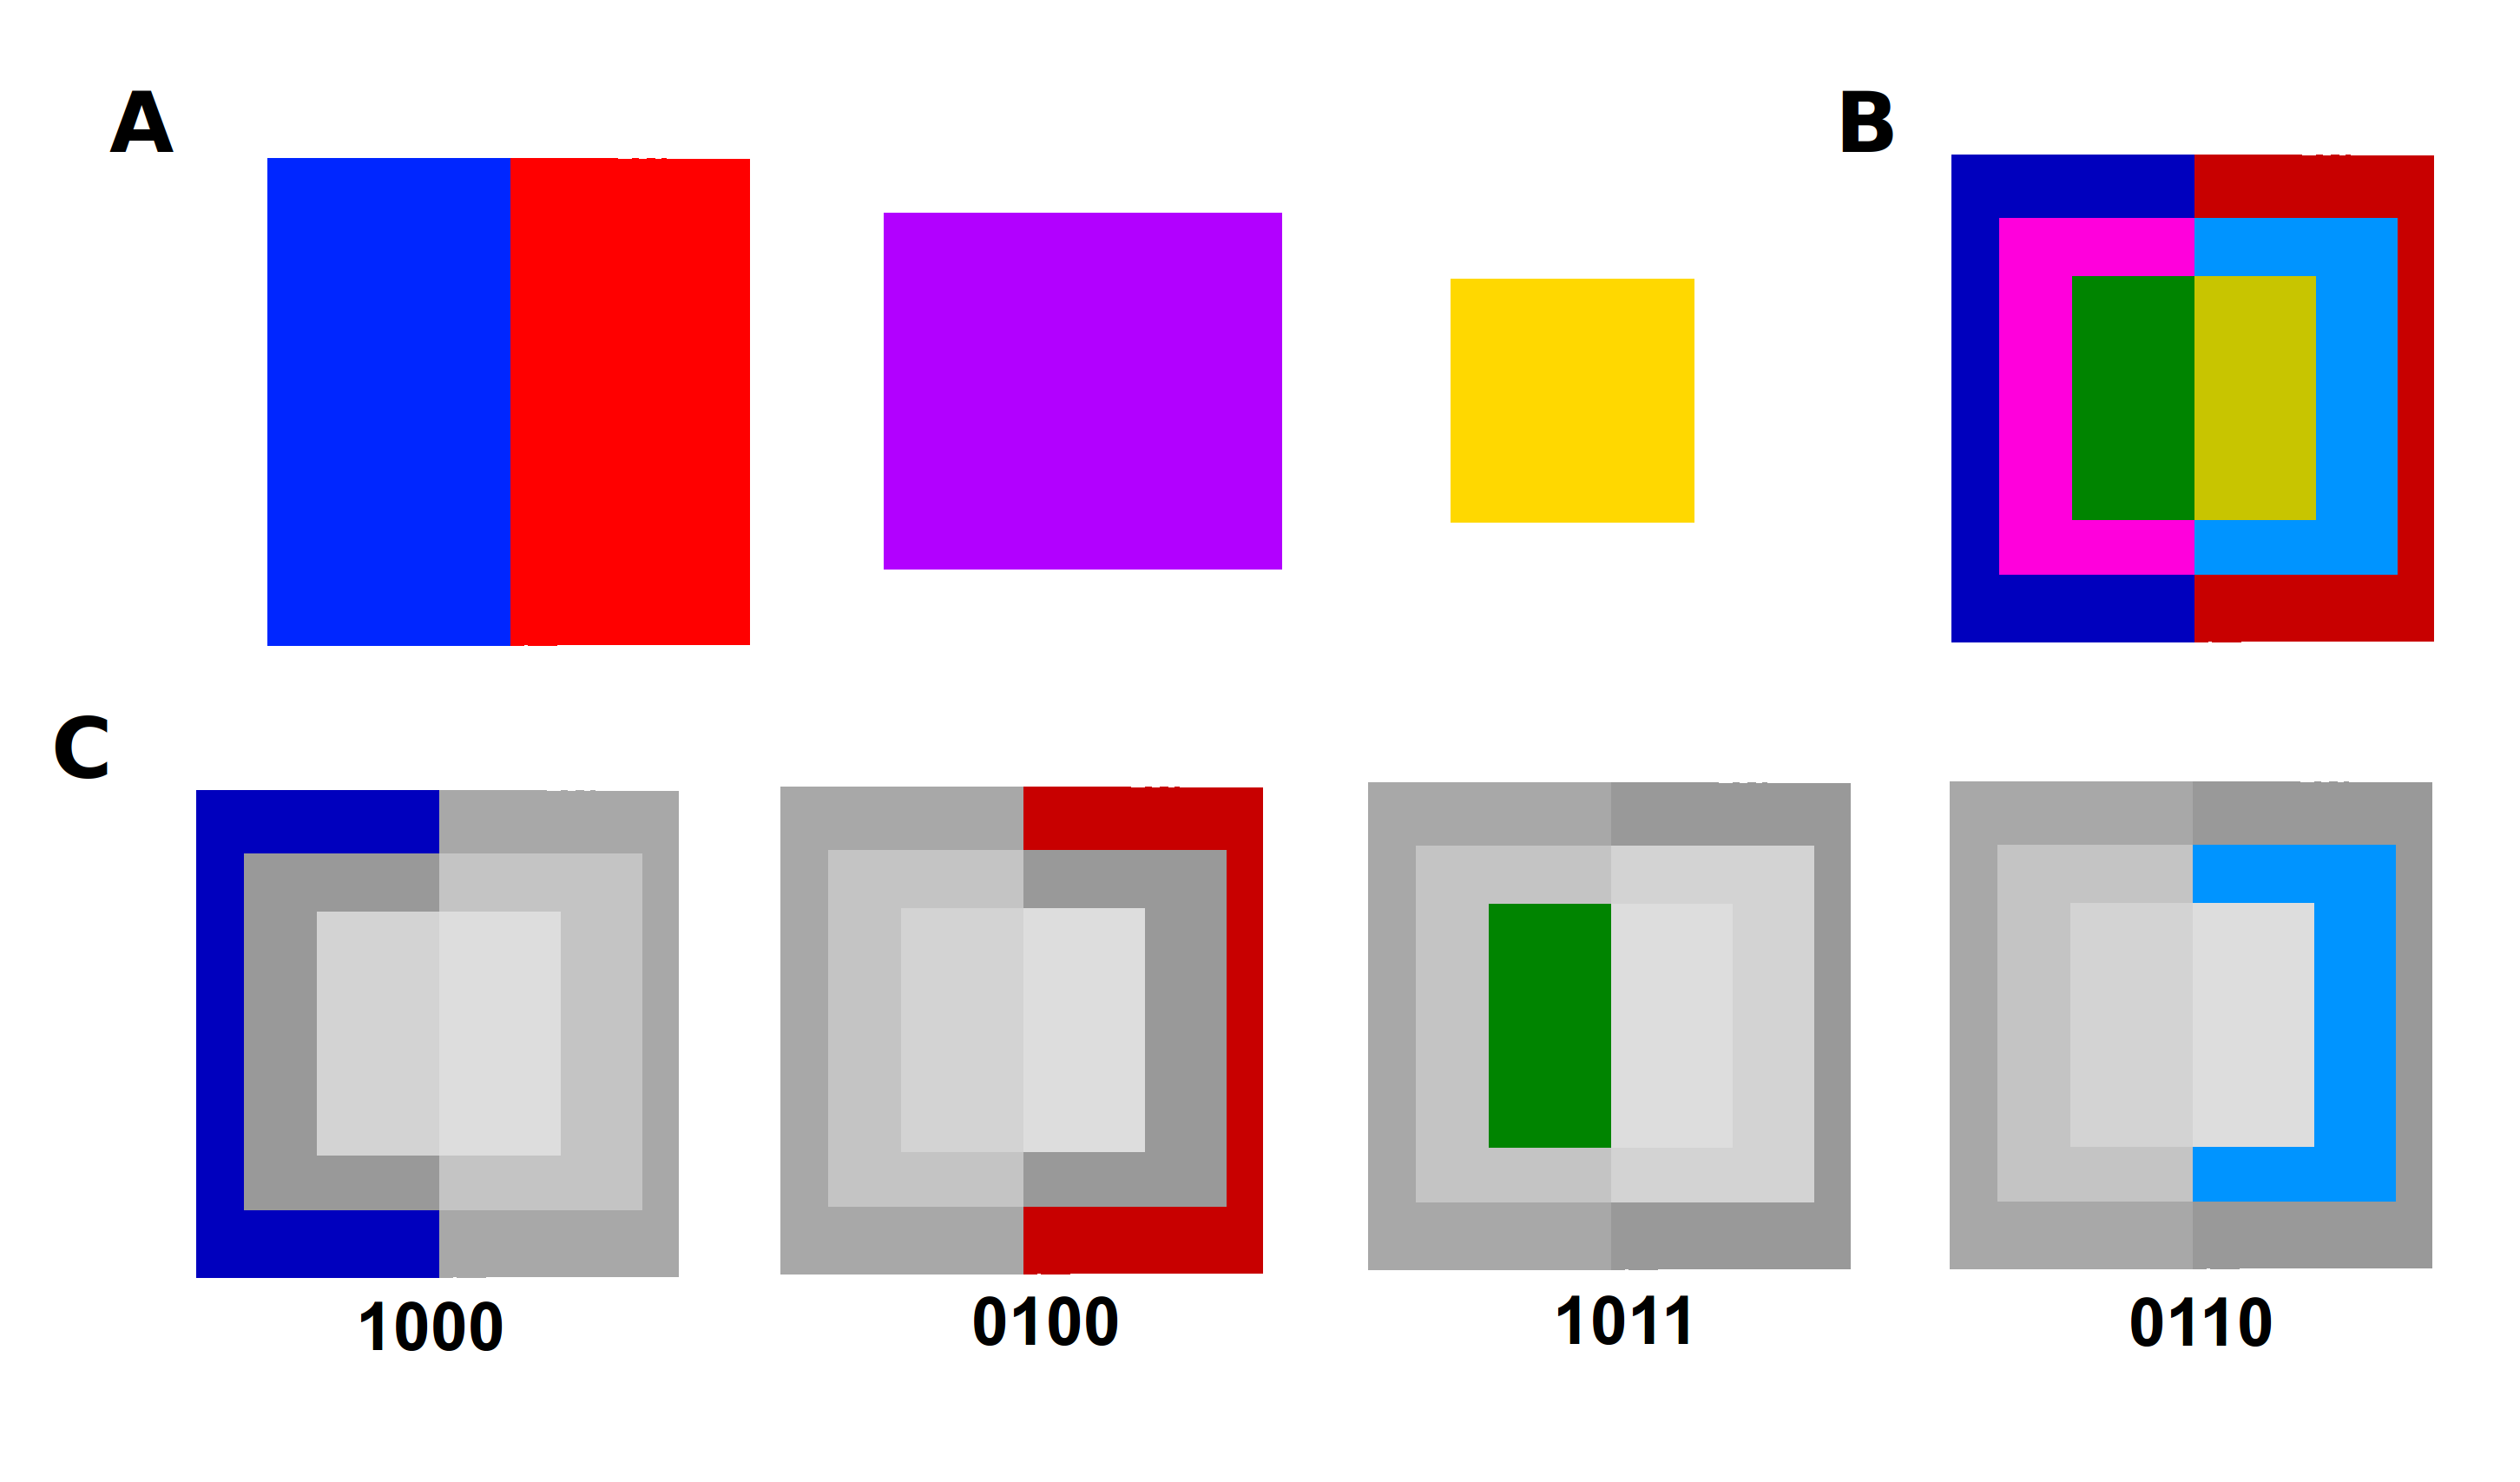
\includegraphics[width=0.95\textwidth]{./graphics/chp4/dot.png}
%  \caption{The upper left panel, A), shows colored squares, each
%    schematically representing a domain enclosed by a surface. The
%    left hemisphere is blue, the right hemisphere is red, the white
%    matter is purple, the ventricles are yellow, and their bounding
%    surfaces are given in this order. The upper right panel B) shows the
%    combination of each colored square. The bottom panel C) shows four
%    different subdomains and its corresponding bit-string. The left
%    image, 1000, denotes the volume that is within the left
%    hemisphere, but not within the right hemisphere, white matter or
%    ventricles -- hence the gray matter of the left hemisphere. The
%    image 0100 is completely analogous for the right hemisphere. Then
%    1011 refers to the surface that is within the left hemisphere
%    and within both the white surface and ventricles; hence the left
%    ventricle. Finally, 0110 represents the white matter of the
%    right hemisphere. }
  \caption{The upper left panel, (A), shows three colored squares that 
	differentiate the volumes enclosed by the large scale surfaces 
	files, in the \pythoninline{surfaces} list, at their simplest level.  
	The left hemisphere volume is colored blue, the right hemisphere volume 
	is colored red, the white matter volume is purple and the ventricle 
	volume is yellow.  The upper right panel (B) shows the complex 
	combination of volumes that can be separately tagged using 
	\pythoninline{smap.add} and the surfaces defined in the 
	\pythoninline{surfaces} list.  The regions of (B) are colored by an 
	independent color scheme that shows all possible combinations, of 
	volumes, addressable by \pythoninline{smap.add}.  The bottom panel (C) 
	shows four, of the six, different subdomains of (B) and their corresponding bit 
	strings. The left image, corresponding to bit string `1000', denotes 
	the volume that is within the left hemisphere, but not within the right 
	hemisphere, white matter or ventricles -- hence the gray matter of the 
	left hemisphere.  The image with bit string `0100' is completely 
	analogous for the right hemisphere. The bit string `1011' refers to the 
	surface that is within the left hemisphere and within both the white 
	surface and ventricles; hence the left ventricle. Finally, the image 
	for the bit string `0110' corresponds to the white matter of the right 
	hemisphere. For completeness, the remaining two bit strings for the 
	regions shown in (B) are `1010' (left, magenta region) and `0111' 
	(right, golden region).}
\label{fig:chp4:smap-example}
\end{figure}

To represent the subdomains, assuming that \pythoninline{lpial, rpial,
  white}, and \pythoninline{ventricles} exist as
\pythoninline{svmtk.Surface}s, we could use the following sample code:
\begin{python} 
surfaces = [lpial, rpial, white, ventricles]
smap = svmtk.SubdomainMap()
\end{python}
The ventricles are filled with cerebrospinal fluid.  A practical motivation for 
tagging the ventricles separately may be, for example, a desire to specify a 
much faster (isotropic) diffusion coefficient in the ventricular domain.  Here, 
we demonstrate the marking all of the mesh tetrahedrons that lie inside the 
subdomain defined by the ventricle surface with a (tag) value of 6. To do this, %
%To mark all the tetrahedra in the ventricles in the left hemisphere
%with the tag value 6, 
%we need to identify the placement of the left ventricles within the ordered 
%list of surfaces
we need to identify the placement of volume corresponding to the left 
ventricles; as we have seen, this volume is defined implicitly by the surfaces 
within the list \pythoninline{surfaces}.  The ventricles in the left hemisphere are inside the left 
pial surface, outside the right pial surface, inside the gray-white matter 
surface and inside the ventricular surface, resulting in the bit-string "1011". 
We could thus call \pythoninline{smap.add} as 
\begin{python}
smap.add("1011", 6)
\end{python}
Similarly, we can tag the ventricle volume within the right pial
surface by
\begin{python}
smap.add("0111", 6)
\end{python}
Finally, we can tag the ventricular volume at the intersection of the
left and right pial surfaces via
\begin{python}
smap.add("1111", 6)
\end{python}
Indeed, tagging the entire ventricular volume in this manner requires that we add all
three of the lines above.

Finally, we note that {\svmtk} also allows for marking several
domains at once:
\begin{python}
smap.add("10*", 6)
\end{python}
will mark all underlying domains, that is, in this case "1000", "1001",
"1010", and "1011".  Note that the use of the asterisk requires a
prior specification of the number of input surfaces, either as an
optional argument in the constructor, of a \pythoninline{SubdomainMap} object 
such as \pythoninline{smap}, or by using the member function 
\pythoninline{set\_number\_of\_surfaces} of the \pythoninline{SubdomainMap} 
class (for example,  \pythoninline{smap.set\_number\_of\_surfaces}). Therefore, 
as an alternative, one could just include the line
\begin{python}
smap.add("*1", 6)
\end{python}
instead of adding each ventricular volume separately.

\section{Separating the ventricles from the gray and white matter}
\label{sec:chp4:tools:remove-vent}

The volume hemispheric meshes created in Chapter~\ref{chp:chp3}, and the
volume hemisphere mesh illustrated in 
Figure~\ref{fig:chp4:ernie-tagged-twodomain-mesh} include the
ventricles as part of the white matter. Since the physics of the
fluid-filled ventricles and the soft but solid brain cerebrum may be
very different, removal of the ventricles from the hemisphere volume
is a useful operation. Here, we demonstrate how to (i) use
{\freesurfer} to extract and postprocess the ventricular surface, and
(ii) remove the resulting ventricular volume from the cerebrum.

\subsection{Extracting a ventricular surface from MRI data}
\label{sec:chp4:tools:remove-vent:extraction}  

We will extract the ventricle surface(s) from our T1 MRI data via
{\freesurfer}. Extracting a ventricular surface representation is
relatively straight-forward, while extracting a high-quality surface
representation may be more involved. We therefore introduce tools and
utilities of increasing complexity.

\subsubsection*{Segmentations and parcellations: A sneak peek}
\index{segmentation} \index{parcellations}
\index{FreeSurfer!\emp{recon-all}} Recall that \freesurfer's
\emp{recon-all} generates a number of surface and volume files (see,
for example, Chapter~\ref{sec:chp3:surfaces}). In particular, the
\freesurfer{}-generated \emp{mri/} directory includes volume-based
data, such as T1-weighted images, segmentations, and
parcellations. These volume files have the extension \emp{mgz}, and
the segmentations and parcellations can be identified by the base
filename. For instance, the file \emp{aseg.mgz} stands for automatic
segmentation, and the file \emp{wmparc.mgz} stands for white matter
parcellation. The parcellation will split the segmentation into finer
regions, for example, the cortical gray matter will be divided into 35
regions\footnote{FreeSurfer defines regions via an anatomical atlas.  An 
atlas is a labeling of distinct regions.  The 35 regions referenced here 
correspond to the Desikan-Killiany atlas which ships with FreeSurfer; 
the Destrieux atlas also ships with FreeSurfer and can be used to annotate 
various cortical regions.  More information regarding FreeSurfer atlas 
annotations is available at 
\url{https://surfer.nmr.mgh.harvard.edu/fswiki/CorticalParcellation}} %
for each hemisphere. We can use the segmentation or the
parcellation files to construct the surface of the ventricular volume.

\index{parcellations!region tags}
The segmentations can be inspected using, for example, Freeview. As an
example, we use the \freesurfer{} generated files from our data set at
\emp{freesurfer/ernie/mri}, and visualize the \emp{aseg.mgz} file:
\terminal{\$ cd freesurfer/ernie/mri \\ \$
  freeview -{}-colormap lut -{}-v aseg.mgz}

\noindent The list in the left hand panel of the Freeview window shows
the segmentation tags, that is, the values associated with different brain
regions. Alternatively, hovering the pointer over a voxel will
cause the corresponding region tag and name to appear in the bottom
right corner. For instance, the left hippocampus has tag 17, while the
fourth ventricle has tag 15. We will look more into segmentations and
parcellations in Chapter~\ref{sec:import-freesurfer-parcellation},
including a visualization in Figure~\ref{fig:chp4:freesurfer-parc}.

\subsubsection*{Extracting and binarizing voxel-based information}
\index{FreeSurfer!\emp{mri\_binarize}}
The {\freesurfer} command \emp{mri\_binarize} is used to extract and
mark voxels that contain a certain type of information such as a range
of signal values or a collection of segmentation tags. The command
includes about 40 optional flags, all of which are described in
\terminal{\$ mri\_binarize -{}-help}

\noindent or via the FreeSurfer online
documentation~\cite{freesurfer-wiki}; we will focus on but a few of
these here.

The input file is given following the flag \emp{-{}-i}, and a volume
output file (\emp{.mgz}) is given following the flag \emp{-{}-o}. A
surface output file (\emp{.stl}) can be given in addition to or
instead of the volume output following the flag \emp{-{}-surf}. The
essential flag \emp{-{}-match}, followed by one or more integers, will mark
all voxels whose assigned segmentation region identification tag matches any of 
the given integer values. For instance, to select all voxels from the fourth 
ventricle, we can use \emp{-{}-match 15}\footnote{{\freesurfer} assigns a numeric 
label to each identified region in the brain. These labels can be viewed by opening a subject's \emp{aseg.mgz} file 
using Freeview.  Doing so, we see that a value of `15' is assigned by 
{\freesurfer} to the region that its segmentation procedure identifies as 
the subject's fourth ventricle.}. 
Alternatively, specific regions can 
also be identified by designated flags, for instance, as follows:
\begin{itemize}
\item \emp{-{}-ventricles} marks voxels in the third and lateral ventricles and in the choroid plexus,
\item \emp{-{}-ctx-wm} marks voxels in the cerebral white matter,
\item \emp{-{}-gm} marks voxels in the gray matter, and  
\item \emp{-{}-subcort-gm} marks voxels in the subcortical gray matter, including the gray matter in the cerebellum and brainstem.  
\end{itemize}
These flags can be combined. For example,
\terminal{\$ mri\_binarize -{}-i aseg.mgz -{}-ventricles -{}-match 15 -{}-o v.mgz}

\noindent will mark the third and lateral ventricles (via the
\emp{ventricles} flag) and the fourth ventricle (with match value
15). In the output file, all the marked voxels will have the value one
and the rest will be set to zero. This result can be changed by specifying the
output bin value with the optional flag \emp{-{}-bin} followed by an
integer. The marked voxels will now have the selected bin value in the
output. The surface output flag \emp{--surf} is often used together
with the flag \emp{-{}-surf-smooth} followed by an integer determining
the number of smoothing iterations on the output surface. 

To extract the ventricular surface from our white matter parcellation,
we define a customizable bash script (\emp{extract-ventricles.sh}). We begin by defining the input and output file names:
\lstinputlisting[style=bashStyle,firstline=1,lastline=5]{../mri2fem/mri2fem/chp4/extract-ventricles.sh}

\noindent To extract a surface file of the ventricular system, we call
\emp{mri\_binarize} with the input filename (in \emp{input}), the \emp{--ventricles} flag, additional tags given by \emp{matchval}, and a number of smoothing iterations:
\lstinputlisting[style=bashStyle,firstline=47,lastline=51]{../mri2fem/mri2fem/chp4/extract-ventricles.sh}

\noindent Prior to this call, we allow for the inclusion of the fourth
ventricle and aqueduct by setting the \emp{matchval} variable\footnote{Setting 
the \emp{matchval} variable only \textit{allows for} the inclusion of the fourth 
ventricle and aqueduct.  In particular, the aqueduct is a small, fine structure 
and is typically not fully differentiated. Note 
that volume files can be edited manually using Freeview, for instance to 
repair a partially resolved or missing aqueduct. See 
\url{https://surfer.nmr.mgh.harvard.edu/fswiki/FreeviewGuide/FreeviewTools/VoxelEdit} 
for more detail.} and we set the \emp{num\_smoothing} iterations:
\lstinputlisting[style=bashStyle,firstline=7,lastline=15]{../mri2fem/mri2fem/chp4/extract-ventricles.sh}

\noindent We suggest setting \emp{num\_smoothing} to an
integer value between one and five. The resulting ventricular surfaces
with zero and five smoothing iterations, both including the fourth
ventricle, are shown in
Figure~\ref{fig:chp4:ernie-ventricles-smoothing-example}.
\begin{figure}
  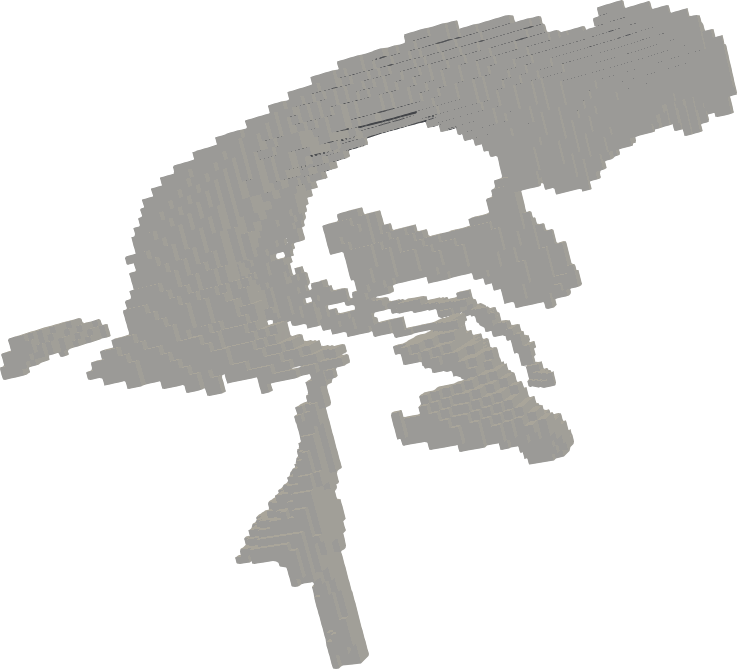
\includegraphics[width=0.49\textwidth]{./graphics/chp4/ernie-vent-0smooth-r.png}
  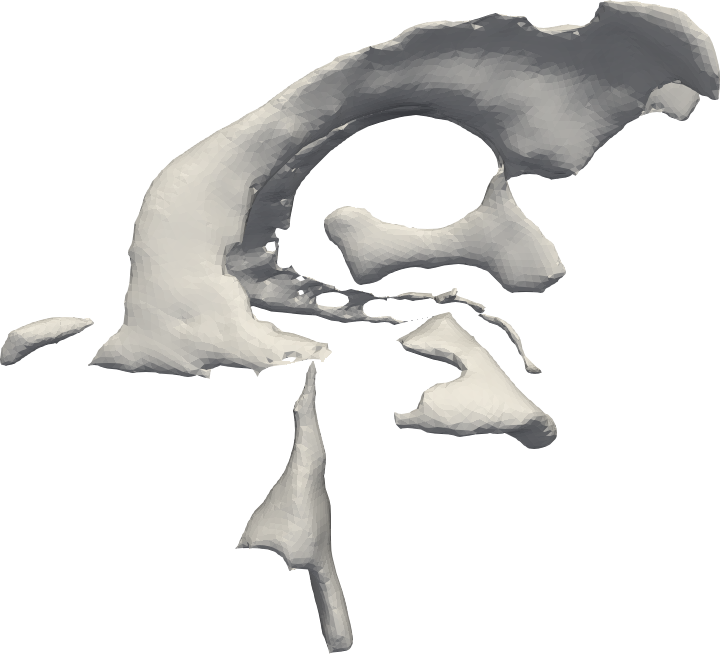
\includegraphics[width=0.49\textwidth]{./graphics/chp4/ernie-vent-5smooth-r.png}
  \caption{Ventricular surfaces, including the fourth ventricle,
    extracted and generated by \freesurfer{} from MRI images. No
    smoothing of the output surface (left) and five smoothing
    iterations (right). Note the disconnected regions.}
  \label{fig:chp4:ernie-ventricles-smoothing-example}
\end{figure}

In practice, the decision to include or discard the fourth ventricle
and aqueduct is data specific. The aqueduct may not be well resolved
in the MRI data on a patient-by-patient basis; if the aqueduct is not
visible in the data then keeping the fourth ventricle leads to a
ventricle system that is not connected, as
Figure~\ref{fig:chp4:ernie-ventricles-smoothing-example} indeed
shows. Moreover, if we include the fourth ventricle and aqueduct,
we should be cautious regarding the extent of the smoothing. 

\subsubsection*{Improving the morphology of the ventricular surface}
\index{connecting surfaces}
\index{FreeSurfer!\emp{mri\_volcluster}}
\index{FreeSurfer!\emp{mri\_morphology}}
In Section~\ref{sec:chp4:tools:remove-vent:removal}, we will use the 
ventricular surface to modify a volume mesh.  In this section, we discuss 
improving the ventricle surface by fixing a few morphological defects that may 
be present following the extraction process.  In particular, we will introduce 
the \freesurfer{} utilities \emp{mri\_volcluster} and \emp{mri\_morphology}.  
These tools can be used to: remove the smaller disconnected ventricle regions 
that may appear in the original surface extraction; close small holes in the 
large ventricle surface; and smooth the resulting surface before further use. 

\begin{itemize}
\item
  \emp{mri\_volcluster} is used to identify clusters in a volume. A
  cluster is defined as a set of continuous voxels that satisfies a
  specified volume threshold criteria; we will specify a minimum volume 
  threshold in the code example below. The input file is given following the 
  flag \emp{-{}-in}, \emp{-{}-thmin} gives a minimum threshold value,
  \emp{-{}-minsize} gives a minimal cluster volume (in
  mm$^3$). Different output flags are
  admissible~\cite{freesurfer-wiki}, including \emp{-{}-ocn}, used to
  save the output volume file with sorted clusters, where all voxels of
  the largest cluster will have the tag 1, the second largest would have
  the tag 2, and so on.
\item
  \emp{mri\_morphology} is used to perform certain operations on
  volume files and supports many operations.  These operations include opening, 
  closing, dilating, eroding and filling holes in a volume.  %We will 
  %illustrate how to use this function below for connecting the extracted 
  %domain by closing holes.
  We will make use of the `close' operation, of this utility, to close holes 
  in an extracted ventricle domain. 
\end{itemize}

Using these functions, we may extract an improved, higher-quality
ventricular surface by removing apparently disconnected regions. Our
algorithm takes the following steps:
\begin{enumerate}
\item
  We extract the lateral and third ventricles into a separate volume
  file.
\item
  In this separate volume, we extract clusters of connected voxels,
  but only those above a minimal cluster size. Since the average adult
  volume of cerebrospinal fluid in the ventricles is about 150
  mm$^{3}$, we set the threshold size to be around 100 mm$^3$.
\item
  We extract the largest of these clusters (thus ignoring smaller,
  disconnected regions)
\item
  We close any holes in the resulting volume as necessary.
\item
  We extract the surface of the resulting volume and smooth it as
  necessary.
\end{enumerate}
The corresponding continuation of our Bash script is as follows. Note
how we output the clusters sorted by size using the argument
\emp{-{}-ocn} to \emp{mri\_volcluster} and extract the largest
cluster by matching on one in the subsequent call to
\emp{mri\_binarize}. We allow for setting the number of closing
iterations \emp{num\_closing} and the minimal largest cluster size
\emp{V\_min} as parameters. We advise setting the number of closing
iterations relatively low (e.g.~to 1 or 2). Setting the number of closing
iterations too high can cause non-physiological connections in the
resulting ventricular surface.
\lstinputlisting[style=bashStyle,firstline=16,lastline=46]{../mri2fem/mri2fem/chp4/extract-ventricles.sh}

\begin{figure}%\sidecaption
  \centering
  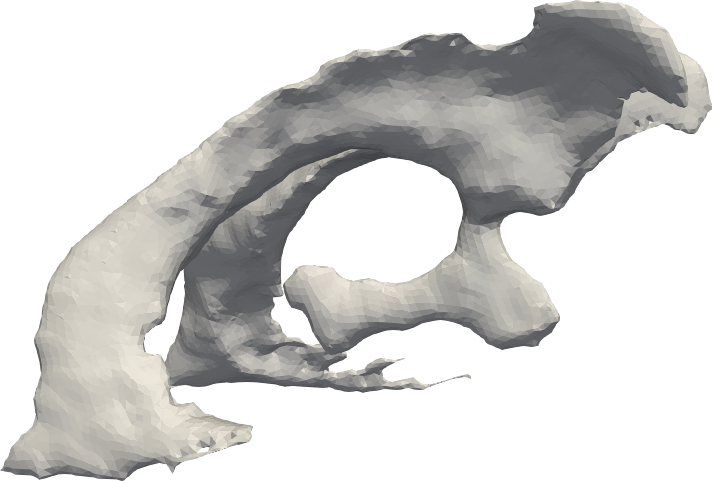
\includegraphics[width=0.75\textwidth]{./graphics/chp4/ernie-ventricles-final-r.png}
  \caption{Post-processed ventricle %High-quality, connected, smooth ventricular surface
    surface extracted from MRI using \freesurfer{}.  This surface file 
    (\emp{ernie-ventricles.stl}) is created by the script 
    \emp{mri2fem/chp4/extract-ventricles.sh}.}
  \label{fig:chp4:ernie-ventricles-final}
\end{figure}
\noindent Figure~\ref{fig:chp4:ernie-ventricles-final} shows the ventricular
surface STL file generated by the above code, with \emp{postprocess=true}, 
visualized in ParaView. 

\subsection{Removing the ventricular volume}
\label{sec:chp4:tools:remove-vent:removal}  
\index{SVM-Tk!\emp{Surface}}
\index{SVM-Tk!\emp{SubdomainMap}}
\index{SVM-Tk!\emp{remove\_subdomain}}
In this section, we demonstrate how to remove a subvolume defined by
an enclosing surface. Though we will focus, here, on removing the
volume enclosed by the ventricle surface, as extracted in the previous
section, the general process will also work for any volume defined by
a closed surface STL file. The core idea is to use \svmtk{} to
generate tags for the different subvolumes in the domain and then
simply delete the volume corresponding to a specific tag.  

We assume that we have the left pial, gray/white matter, and ventricular
surfaces available as STL files. Again, we will wrap the main
functionality in a Python function, called
\pythoninline{create\_gwv\_mesh}, to create the `gray matter plus white matter' 
volume mesh. This 
function can then, for instance, be called as
\newpythonsnippet{chp4}{three-domain-tagged.py}{33}{35}

\noindent This code example is included in
\emp{mri2fem/chp4/three-domain-tagged.py}.

We first create \pythoninline{Surface}s from the surface STL files:
\newpythonsnippet{chp4}{three-domain-tagged.py}{1}{10}

\noindent We then tag different regions using \pythoninline{SubdomainMap}: 
\newpythonsnippet{chp4}{three-domain-tagged.py}{12}{19}

\noindent As before, we create a tagged mesh (of a given resolution)
of the domain via the surfaces and the subdomain map:
\newpythonsnippet{chp4}{three-domain-tagged.py}{21}{24}

We can now, via a call to \svmtk{} \pythoninline{remove\_subdomain},
remove the mesh cells tagged as within the ventricles before saving
the mesh:
\newpythonsnippet{chp4}{three-domain-tagged.py}{26}{31}
Note that \pythoninline{remove\_subdomain} can also handle the removal of
multiple subdomains by providing a tuple of tags as input. The resulting
meshes, with and without ventricles removed, are shown in Figure
\ref{fig:chp4:tags-with-without-ventricles}.
\begin{center}
\begin{figure}
  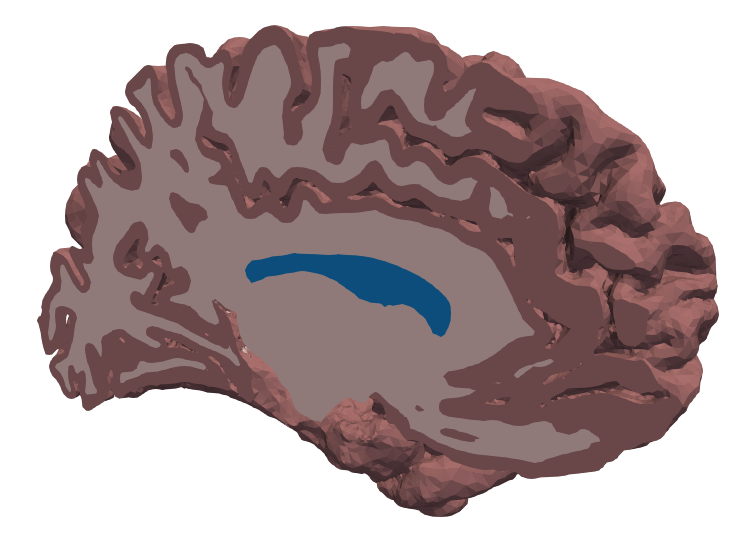
\includegraphics[width=0.49\textwidth]{./graphics/chp4/ernie-final-comp-b}
  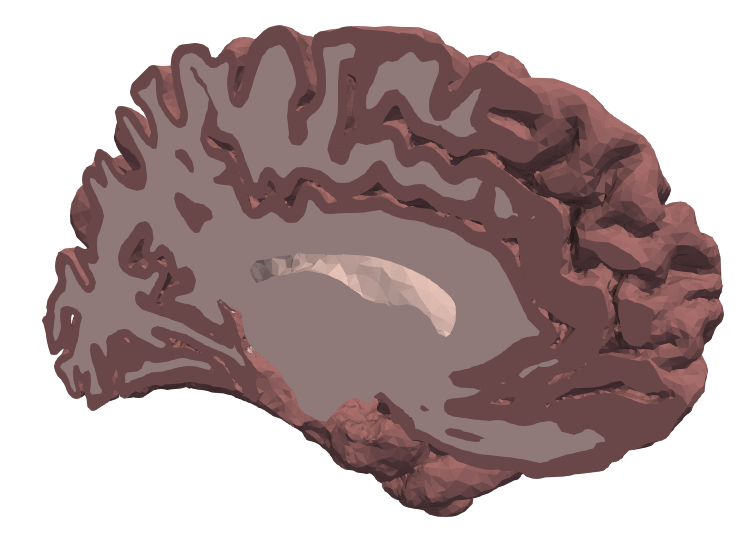
\includegraphics[width=0.49\textwidth]{./graphics/chp4/ernie-final-comp-d}
    \caption{Volume meshes of the left hemisphere (sagittal planes),
      conforming to the gray matter, white matter, and ventricles, with
      ventricles marked in blue (left) and with ventricles removed (right).  
	Note: that the tetrahedral boundary lines of the mesh have been 
	suppressed for visual clarity.  To view the tetrahedra of the mesh, 
	select the \emp{Surface With Edges} option, for the \emp{Representation} 
	setting in the left hand pane, after loading the \emp{.mesh} files, 
	created by \pythoninline{three-domain-tagged.py}, in ParaView. 
	}
    \label{fig:chp4:tags-with-without-ventricles}
\end{figure}
\end{center}

\section{Combining the hemispheres together}
\label{sec:chp4-left-right-tagged}

In this section, our aim is to create a mesh that includes both the
left and right hemispheres, with gray and white regions tagged, and
the ventricular volume removed. We will combine the approaches of the
previous sections with \svmtk{} techniques for
working with the union of multiple surfaces. 

\subsection{Repairing overlapping surfaces}
\index{repairing surfaces}
\freesurfer{} generates the right and left hemisphere surfaces
separately. Combining surfaces from different hemispheres
can therefore create problems, such as
\begin{itemize}
\item The hemisphere surfaces overlap, creating bridges in the cortical gray 
matter, at the mesh and surface level, that do not exist physically.
\item The hemisphere surfaces may have gaps between them which are too large 
and are unphysical. In this case, the resulting mesh may undesirable gaps 
between the hemispheres where they would otherwise be connected by the 
white matter nerve tracts.  
\end{itemize} 
In general, we want to join the hemisphere surfaces, via the white matter 
nerve tracts, while simultaneously avoiding overlapping surfaces in the 
cortical gray matter.  %We can consider this a combined problem, since we 
%typically would want to join the hemisphere surfaces via the white matter 
% nerve tracts, while avoiding overlapping surfaces in the cortical gray matter. 
\svmtk{} includes utilities for addressing such challenges. In particular,
\begin{itemize}
\item
  \pythoninline{separate\_overlapping\_surfaces} can separate
  overlapping surfaces,
\item
  \pythoninline{separate\_close\_surfaces} can separate nearly-%
  overlapping surfaces, and
\item
  if we desire a single surface for the white matter but the white matter 
  surfaces only partially overlap, due for instance to smoothing, the 
  \svmtk{} function \pythoninline{union\_partially\_overlapping\_surfaces} 
  offers an improved set of features to handle the union operation of 
  the white matter surfaces.
%
%  if the surfaces partially overlap, due for instance to smoothing, and we 
%  want to create a single surface 
% 
%  if we want to create a single surface for the white matter but the
%  surfaces only partially overlap due to smoothing,
%  \pythoninline{union\_partially\_overlapping\_surfaces} offers
%  improved features to handle the union of white matter surfaces.
\end{itemize}
The following code snippet illustrates an example of the usage of these functions:
\begin{python}
# Input Surfaces
rpial = svmtk.Surface("rh.pial.stl")
lpial = svmtk.Surface("lh.pial.stl")
rwhite = svmtk.Surface("rh.white.stl")
lwhite = svmtk.Surface("lh.white.stl")

# Create white matter surface as union of hemispheres
white = svmtk.union_partially_overlapping_surfaces(rwhite,
                                                   lwhite)

# Separate overlapping and close vertices between
# the left and right pial surfaces,
# but only outside the optional third argument, which
# in this example is the white surface:
svmtk.separate_overlapping_surfaces(rpial, lpial, white)
svmtk.separate_close_surfaces(rpial, lpial, white) 
\end{python} 

\subsection{Combining surfaces to create a brain mesh}
We assume that left pial, left white, right pial, right white and
ventricular surface STL files have been extracted, converted and
possibly processed, by the processes described in the previous
section. Now, how do we combine these to create a complete brain mesh?

Again, we proceed via an \svmtk{} code example (with the complete
code included in \emp{mri2fem/chp4/fullbrain-five-domain.py}). We wrap
the main functionality in a Python function
\pythoninline{create\_brain\_mesh}. This function can then, for
instance, be called as:
\newpythonsnippet{chp4}{fullbrain-five-domain.py}{42}{45}

We begin by loading \emp{Surface}s from the STL files. 
\newpythonsnippet{chp4}{fullbrain-five-domain.py}{0}{7}
We take the union of the left and right white surfaces to illustrate
the possibility of combining surfaces:
\newpythonsnippet{chp4}{fullbrain-five-domain.py}{9}{15}
It is natural to ask whether we can do the same with the pial matter;
indeed, the union of the left and right pial surfaces is
possible. However, generally, whether one can successfully mesh the
joined surface, without further postprocessing, is data specific.
There is a higher chance that the {\freesurfer} segmentation process
of the left and right pial MRI surface data can lead to non-physical
intersections, thus producing left and right pial surface files that
overlap and self-intersect when combined.  Self-intersections within
a surface can then cause the meshing process to fail. Similarly, one
could simply work with all five surfaces separately.  This approach 
leads to a more complex tagging process, with \emp{SubdomainMap}, but
alleviates difficulties, such as the self-intersections mentioned above, 
that can arise when computing the union of two surface objects.

We continue by creating tags, a subdomain map, domain and mesh, and
leave the option of removing the ventricles, as in previous examples:
\newpythonsnippet{chp4}{fullbrain-five-domain.py}{17}{40} Note that
running this code example as is will take some time, on the order of a
few minutes. The resulting mesh can be visualized using ParaView
after conversion from .mesh to .vtu or .xdmf.

\section{Working with parcellations and finite element meshes} 
\label{sec:import-freesurfer-parcellation}
\index{parcellations}
{\freesurfer}'s \emp{recon-all} automatic segmentation process can identify 
almost two hundred different brain regions\footnote{{\freesurfer}'s \emp{recon-all} parcellates a brain into the regions 
defined by the Desikan-Killiany and Destrieux atlases.  Numbers are assigned 
to the different regions, by default, when \freesurfer{} performs the 
segmentation. These numbers are specific to \freesurfer{} but independent of a 
subject.  We note that the particular brain matter that \freesurfer{} 
identifies as `region N' (where N is some number) may differ between patients 
depending on their individual brain topology.}.  {\freesurfer} labels 
identified regions with a numeric code.  For instance, in the left 
hemisphere, \freesurfer{} assigns the numeric code of 17 to the 
hippocampus\footnote{In many
  neuroscience applications, the hippocampus region is of special
  interest because it is central to memory consolidation. The reader
  is refered to the interesting story of Henry Molaison, aka Patient
  H.M.,~\cite{squire2009legacy, scoville1957loss} who lost his ability
  to form new memories after the removal of both the left and right
  hippocampus. The procedure was performed as a treatment for his
  epilepsy. He lived for more than 50 years after the removal of his
  hippocampus and participated voluntarily in many scientific
  experiments, demonstrating the crucial role of the hippocampus. He
  never recognized the scientists who frequently visited him.}, 1035
to the gray matter insula, 3035 to the white matter insula, 1028 to
the gray matter superiorfrontal region and 3028 to the white matter
superiorfrontal region. Figure~\ref{fig:chp4:freesurfer-parc} (left) illustrates 
some of these regions using \emp{freesurfer/ernie/mri/wmparz.mgz} as an example. 
%
%An illustration of some of these regions,
%using \emp{freesurfer/ernie/mri/wmparz.mgz} as an example, is shown in
%Figure~\ref{fig:chp4:freesurfer-parc} (left).
%
\begin{figure}
\begin{center}
  \hspace{2em}
  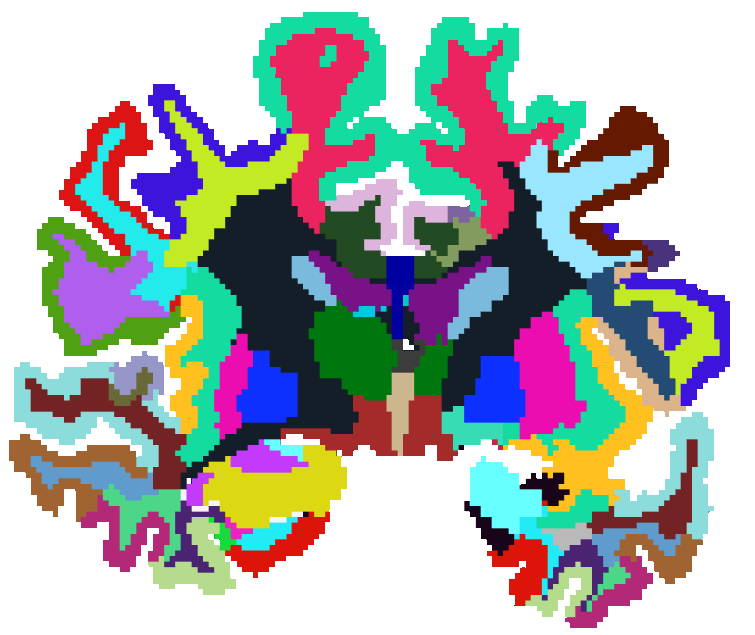
\includegraphics[height=4cm]{./graphics/chp4/parcellation-coronalwhiteBG_2.png}
  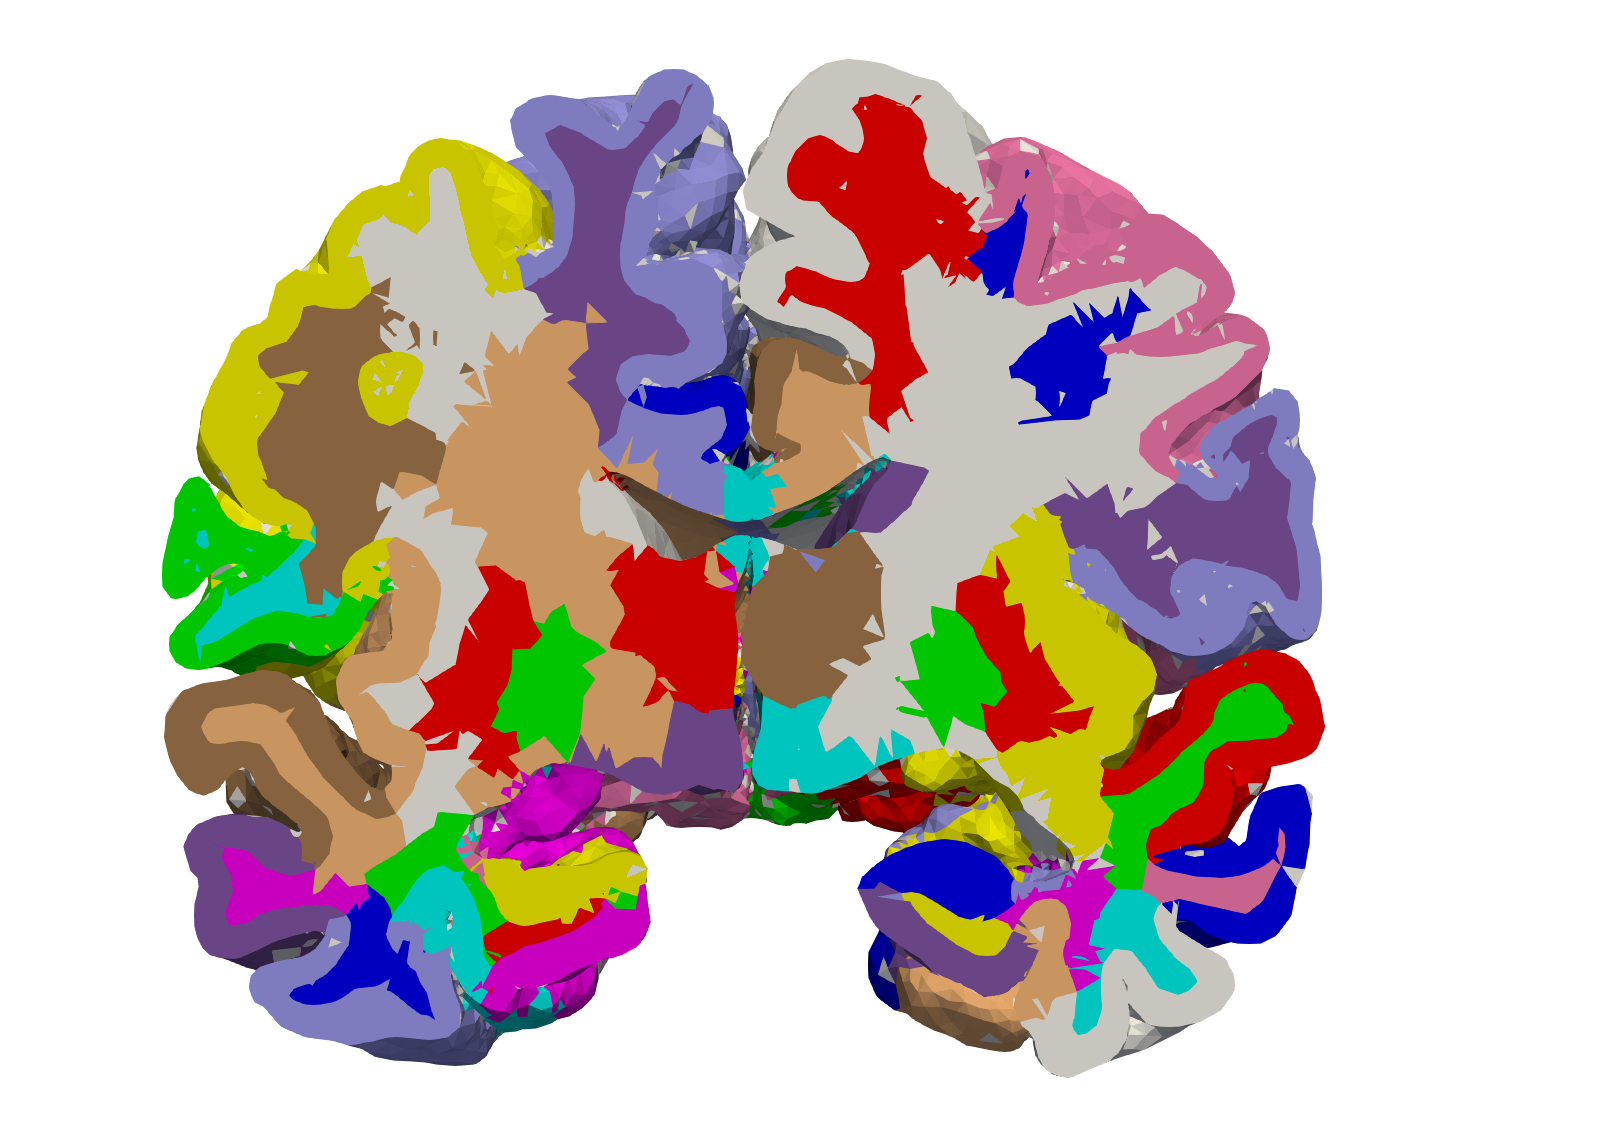
\includegraphics[height=4cm]{./graphics/chp4/ernie32-parcellation-basic.png}
  \caption{Brain parcellations: (left) as generated by \freesurfer{} and visualized 
   using Freeview and (right) the same parcellation transferred onto the {\fenics} 
   brain mesh and visualized using ParaView (with different colors, different 
   slices, and different view angles).} 
    %
    %Left: Parcellation as generated
    %by \freesurfer{} and visualized using Freeview. Right: Same
    %parcellation transferred onto the FEniCS brain mesh and visualized
    %using ParaView. (Different coloring, different slices, different view angles.)}
  \label{fig:chp4:freesurfer-parc}
\end{center}
\end{figure}

\subsection{Mapping a parcellation onto a finite element mesh}
\label{sec:chp4:mapping_parcellation}
\index{FEniCS}
In a brain parcellation, each region is identified by an integer
value. Our current goal is to map these region tags onto the
generated volume mesh and into a FEniCS-compatible format. Doing so
involves
\begin{itemize}
\item
  Reading and working with image (voxel-based) data in Python, 
\item
  Representing discrete mesh data in {\fenics},
\item
  Mapping values from voxel indices, namely, voxel space to mesh coordinates, %
  namely, left-to-right, posterior-to-anterior, inferior-to-superior (RAS) space.
\end{itemize} 
As usual, we will illustrate these steps using a concrete code example
(included in \emp{mri2fem/chp4/map\_parcellation.py}). We wrap our
main functionality in a Python function
\pythoninline{map_parcellation_to_mesh} taking the parcellation
filename and mesh filename as input (with \emp{wmparc.mgz} and
\emp{ernie-brain-32.xdmf} from the previous section as an example).
\newpythonsnippet{chp4}{map_parcellation.py}{64}{65}

\subsubsection*{Working with image data in Python}

\index{nibabel}
\index{FEniCS}
We will use the Python packages NiBabel to work %for working 
with neuroimaging data, NumPy for general numerics in Python, and {\fenics} to 
represent the mesh and the mesh data:
\newpythonsnippet{chp4}{map_parcellation.py}{1}{4}

\noindent We begin by loading the image data from the parcellation
file as follows:
\newpythonsnippet{chp4}{map_parcellation.py}{6}{10}

\noindent We can, for example, inspect the image shape (number of voxels in
each dimension) and extract voxel values by indexing the
\pythoninline{data} array:
\newpythonsnippet{chp4}{map_parcellation.py}{12}{16}

\subsubsection*{Representing discrete mesh data in FEniCS}
\index{FEniCS!\emp{MeshFunction}}
We aim to map the parcellation labels, generated by \freesurfer{} during 
segmentation, onto the brain mesh.  At this point, we have loaded a 
the \freesurfer{} \emp{wmparc.gz}; this parcellation was created from a 
set of T1 MR images.  We will also work with a mesh file; here, that 
file is \emp{ernie-brain-32.xdmf}.  This mesh file was generated from 
surfaces extracted from files which were also constructed, by \freesurfer{}, 
from a set of T1 images. We mention this because the following fact is 
important: to label a mesh file with parcellated region IDs, it is imperative 
that the T1 images used to generate the parcellation and the T1 images used 
to generate the mesh file are the same set of images. 
%
%We aim to map these labels onto the brain mesh generated from the same
%T1 images.


One way to associate discrete data, such as a parcellation label, with mesh 
elements is to use a {\fenics} \emp{MeshFunction}.
%FEniCS offers the concept of a \emp{MeshFunction} to represent such discrete 
%data.  
Mesh functions can be associated with geometrical objects, $X$, of various 
dimensions, $d = \text{dim}(X)$.  We can associate mesh functions with cells 
($d=3$), faces ($d=2$), edges ($d=1$), or vertices ($d=0$). Here, 
we aim to identify the parcellation region for each cell in the brain mesh and 
will thus make use of a cell function. We first import the full brain mesh:
\newpythonsnippet{chp4}{map_parcellation.py}{17}{21}

\noindent  Next, we create a mesh function for the mesh entities of dimension 
3 (tetrahedral mesh cells). Our \emp{MeshFunction} object will  
define a function whose input is a tetrahedron of the mesh and whose 
output, or associated value, is a real number; we start by specifying a 
mesh function associating an initial value of zero to all tetrahedrons of the 
mesh:  
\newpythonsnippet{chp4}{map_parcellation.py}{23}{27}
Note that the \emp{MeshFunction} can be indexed directly, or its values can be
accessed via the member function \emp{array}.

Our strategy, now, is: iterate over all cells in the mesh; identify the 
parcellation region label for each mesh cell; and set the associated value 
of the mesh function, for that cell, to the corresponding parcellation label 
value.  %
%We now aim to iterate this process over all cells in the mesh (function), 
%identify the corresponding parcellation region, and insert this value into 
%the \emp{regions} mesh function. 
However, at this point, a key question arises: While we can index the image's 
data by its indices and the mesh by its cell or vertex indices (and/or their 
coordinates), how can we identify the voxel index corresponding to a given 
cell or vertex (coordinate), and vice versa? 

\subsubsection*{Converting between indices, coordinates, and spaces}

\index{voxel space}
Converting between voxel indices and other coordinates is a core
problem that we will encounter several times. To address this task, we
begin by introducing some nomenclature. The span of the image
dimensions is often referred to as the (T1) \emph{voxel space}, with
indices (or dimensions) $(i, j, k)$. On the other hand, the span of
the mesh axes defines the RAS (left-to-\underline{r}ight, 
posterior-to-\underline{a}nterior, inferior-to-\underline{s}uperior) space 
with coordinates $(x, y, z)$. 

\index{FEniCS!HDF5}
We aim to
construct the transformation $f$ from voxel space to RAS space:
\begin{equation}
  (x, y, z) = f(i, j, k),
\end{equation}
as well as its inverse, $f^{-1}$, from RAS to voxel space. Fortunately,
the parcellation information allows us to extract this transformation easily:
\newpythonsnippet{chp4}{map_parcellation.py}{29}{33}

\noindent Note that FreeSurfer operates with several coordinate
systems, including different RAS spaces. In this book, RAS space will
refer to the FreeSurfer surface RAS space, which is identified
via the suffix \pythoninline{tkr} in the code snippet above.

Next, we iterate over the cells of the mesh.  For each cell, we will: 
extract the cell index; extract the RAS coordinates of the cell 
midpoint; convert from the RAS coordinates to voxel space (via a call to 
\emp{apply\_affine}); round off to the nearest integer values to find the 
image indices; and map the corresponding image data values into the 
\emp{regions} mesh function.  The code for this iterative process is
\newpythonsnippet{chp4}{map_parcellation.py}{35}{50}

We save the resulting mesh function in XDMF format (suitable for
ParaView) and in the HDF5 format (suitable for further FEniCS processing): 
\newpythonsnippet{chp4}{map_parcellation.py}{51}{62}
The result can be seen alongside the original parcellation in
Figure~\ref{fig:chp4:freesurfer-parc}.

\subsection{Mapping parcellations respecting subdomains}
\label{chp4:parcellations}

By careful inspection of the mesh-based representation of the
parcellation in Figure~\ref{fig:chp4:freesurfer-parc} (right), we find
some artifacts in the labeling of the cells. Indeed, since the finite
element mesh is not aligned with the segmentation, the previous direct
mapping between cell midpoints and voxels can lead to minor
inaccuracies. In this section, we therefore aim to improve on our mesh-based
parcellation representation by using subdomain
information. 


Concretely, we aim to do the following
\begin{itemize}
\item
  Read in a mesh with subdomain information.  The mesh may contain many 
  subdomains, such as those defined by a regional parcellation label.  The 
  mesh subdomain structure may also be simple, such as the gray / white matter
  subdomain regions discussed in~Section~\ref{sec:chp4:tools:gray-white:mesh-creation} 
\item
%  Iterate the process over the cells in each subdomain separately and calibrate
%  the voxel values against those of neighboring cells; and
  For each cell in every subdomain, determine if we should alter the label 
  assigned to the cell by inspecting the label of the neighboring cells 
\item
  Store the subdomain and parcellation information together.
\end{itemize}

\subsubsection*{Converting meshes and mesh data between different formats} 
\label{chp4:meshio-converting}

\index{meshio}
\index{FEniCS!\emp{Mesh}}
In Chapter~\ref{sec:chp4:tools:gray-white}, we created a mesh with
gray and white matter labels stored as subdomain information in the
.mesh format. Our next step is to convert this information to a
FEniCS-compatible format. We will write a convenient Python script for this
common operation and use the opportunity to illustrate the use of an
\pythoninline{ArgumentParser} to read in arguments from the command
line, instead of coding the arguments directly into the script
(included in \emp{mri2fem/chp4/convert\_to\_dolfin\_mesh.py}).

%We begin by importing the relevant Python packages, namely, \emp{argparse},
%\emp{meshio}, and \emp{dolfin}:
In this script, we will use the \emp{argparse} package to enable us to pass in 
command-line arguments that inform the conversion process.
\newpythonsnippet{chp4}{convert_to_dolfin_mesh.py}{1}{3}

\noindent Our argument parser set-up looks like this:
\newpythonsnippet{chp4}{convert_to_dolfin_mesh.py}{53}{59}
\noindent and we then  call two functions (described below): 
\newpythonsnippet{chp4}{convert_to_dolfin_mesh.py}{61}{63}
The script can then be called as, for example, 
\terminal{\$ cd mri2fem/chp4\\
\$ python convert\_to\_dolfin\_mesh.py -{}-meshfile ernie-gw.mesh -{}-hdf5file ernie-gw.h5}

We use meshio to first read the .mesh file, its data associated with
the mesh cells (\pythoninline{subdomains}), and its data associated with mesh
facets (\pythoninline{boundaries}). We then write these in the FEniCS-readable
.xdmf format as separate files.
\newpythonsnippet{chp4}{convert_to_dolfin_mesh.py}{5}{27}

Subsequently, {\fenics} can read the files \emp{mesh.xdmf} and \emp{subdomains.xdmf}, 
created above, into a \pythoninline{Mesh} object and \pythoninline{MeshFunction} 
object, respectively.  {\fenics} can then write the data from both objects 
into a single \emp{.h5} file:
%.xdmf files into a
%\pythoninline{Mesh} and \pythoninline {MeshFunction}s, and write these
%collectively to a single .h5 file:
\newpythonsnippet{chp4}{convert_to_dolfin_mesh.py}{29}{51}

%These can be read back into FEniCS as follows (with the filename 
%given in \pythoninline{hdf5file}):
The mesh, subdomain, and boundary information, saved above, can be read 
back into {\fenics} as follows (with the filename 
given in \pythoninline{hdf5file}):
\newpythonsnippet{chp4}{add_parcellations.py}{36}{46}

\subsubsection*{Masking data and improved parcellation identification}

Let us now assume that we have available the \emp{mesh},
\emp{subdomains}, as well as the image \emp{data} from the
parcellation file (e.g \emp{wmparc.mgz}) and the RAS to voxel space
transform \emp{ras2vox}, as described in
Chapter~\ref{sec:chp4:mapping_parcellation}. Our next steps are to
\begin{itemize}
\item
  Find the RAS coordinates of all cells (midpoints), and map these to
  voxel space indices and
\item
  Map parcellation values to mesh cells in a manner that ensures that the
  parcellation regions do not extend across subdomains.
\end{itemize}
In particular, for each mesh cell, we will now examine a neighborhood of the
corresponding voxel values to pick the most frequent adjacent one as
the matched parcellation value. 

We first extract all the RAS coordinates of the cell midpoints,
\newpythonsnippet{chp4}{add_parcellations.py}{57}{59}
before converting these to voxel coordinates and indices, as before:
\newpythonsnippet{chp4}{add_parcellations.py}{68}{72}

Now, we create two arrays.  The first array, \pythoninline{vox2sub}, provides 
a map from the index of a voxel to its subdomain tag;  the second array, 
\pythoninline{regions}, will hold the parcellation tags. 
%We create a convenient map from the voxel indices to the subdomain tags and
%the \pythoninline{regions} array to be filled:
\newpythonsnippet{chp4}{add_parcellations.py}{74}{81}

Now we adjust tags by a consensus method.  We do this by applying the following 
algorithm: for a fixed subdomain, iterate over the cells in that subdomain; 
for each cell, examine the voxel data (region label) associated to the neighbors 
of that cell but only those neighbors which also live in the same subdomain; set 
the region of the cell to the most common region of its neighbors.  This 
process is repeated for each subdomain in the mesh; the algorithm is 
implemented below: 
%
%We iterate the process over each subdomain separately, examine the voxel data
%associated with this subdomain only, and determine for each cell the most
%common tag in a neighborhood around its voxel:
%This algorithm is implemented below.
\newpythonsnippet{chp4}{add_parcellations.py}{83}{97}
We can then update the subdomain array
\newpythonsnippet{chp4}{add_parcellations.py}{99}{104}
and store the resulting mesh data again:
\newpythonsnippet{chp4}{add_parcellations.py}{106}{111}

The \pythoninline{adjacent_tag} function reads 
\newpythonsnippet{chp4}{add_parcellations.py}{7}{30}

The complete script is included in
\emp{mri2fem/chp4/add\_parcellations.py} and can be tested, for example, via 
\terminal{\$ python3 convert\_to\_dolfin\_mesh.py -{}-meshfile ernie-brain-32.mesh -{}-hdf5file ernie-brain-32.h5\\
  \$ python3 add\_parcellations.py -{}-in\_hdf5 ernie-brain-32.h5 -{}-in\_parc wmparc.mgz -{}-out\_hdf5 results/ernie-brain-subdomains-tags.h5 -{}-add 17 1028 1035 3028 3035
}

\section{Refinement of parcellated meshes}
\label{sec:chp4:addparcellations}
\index{mesh refinement!adaptive}
\index{FEniCS!\emp{refine}}
\index{FEniCS!\emp{adapt}}

We end this chapter by examining how we can refine the generated
meshes and, in particular, how we can refine local regions. FEniCS
supports global and local mesh refinement and adaptivity through the
functions \pythoninline{refine} and \pythoninline{adapt}. The latter
(\pythoninline{adapt}) is particularly useful for refining mesh
functions and associated mesh data, in addition to the refinement of
the mesh itself. The code snippets presented here are included in
a complete context in \emp{mri2fem/chp4/refine\_mesh\_tags.py}. 

\subsection{Extending the Python interface of DOLFIN/FEniCS}
DOLFIN, the problem-solving interface to FEniCS, provides a C++ and a
Python interface. The Python interface is generated from the C++
interface using pybind11, but the entire C++ API is not
exposed. Instead, a user can generate their own Python bindings fairly
easily. Since parts of the \pythoninline{adapt} interface are not, by
default, available in Python, we illustrate how to use pybind11 to
compile our own FEniCS wrappers here.

We provide Python bindings for the \emp{adapt} function as follows: 
\newpythonsnippet{chp4}{refine_mesh_tags.py}{4}{18}

We also notice that this function is overloaded, and we provide
bindings to three versions with different signatures. After the code is
executed, the bindings are compiled by the Python module. However,
note that the module will not be added to the DOLFIN library, but
resides in the user's local cache.

\subsection{Refining certain regions of parcellated meshes}
It may be desirable to refine a mesh; either globally or within particular 
regions.  In this section, we discuss two options for refinement; global and 
local.  The code snippets in this section can be found in the file 
\pythoninline{refine\_mesh\_tags.py}.  Let us assume that, 
in Python, we have a FEniCS \emp{mesh} with FEniCS mesh functions 
\emp{subdomains} and \emp{boundaries}, for instance, extracted from an .h5 file, 
as illustrated in Chapter~\ref{chp4:parcellations}. 

One option is, then, to refine the mesh globally, meaning that we refine
all the cells of the mesh. We would then also like to refine or adapt the
associated mesh functions to the refined mesh. We can accomplish this
as follows:
\newpythonsnippet{chp4}{refine_mesh_tags.py}{35}{48}

\begin{figure}[t]	
  \begin{center}
    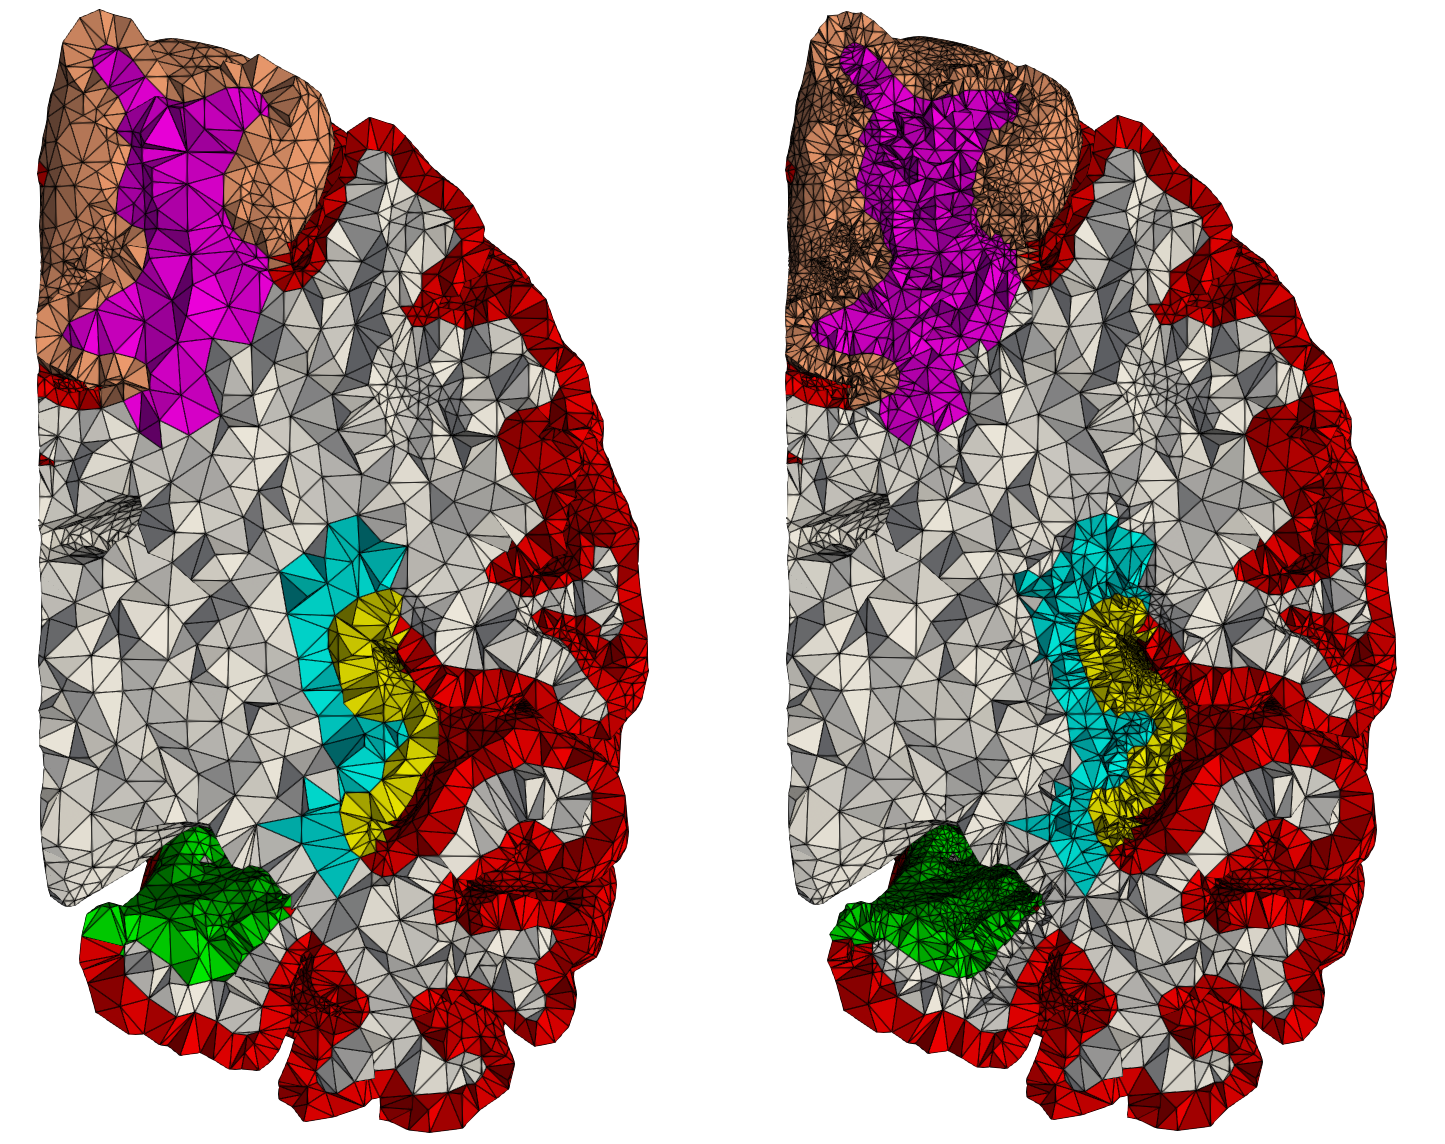
\includegraphics[width=0.7\textwidth]{./graphics/chp4/fenics-parcellation-crinkle.png} \\
    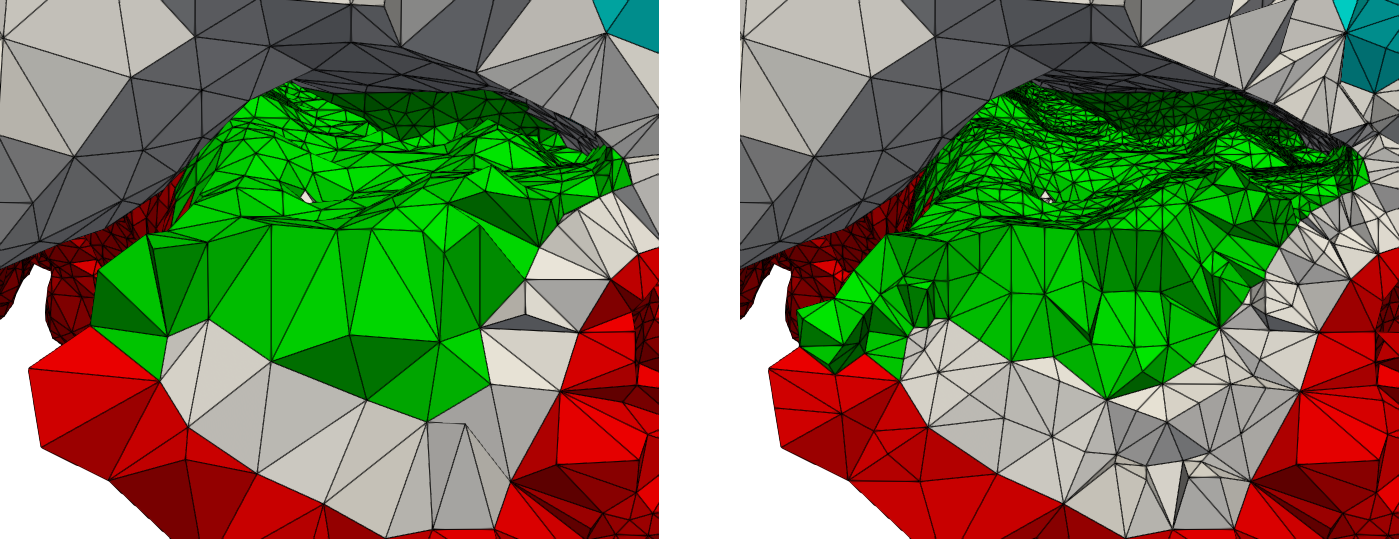
\includegraphics[width=0.9\textwidth]{./graphics/chp4/parcellations_refine_zoom.png}
  \end{center}
  \caption{Illustration of a locally refined left hemisphere mesh.  The left 
  figures show the original mesh with labeled (color coded) regions.  The 
  right figures show the locally refined mesh.  Only particular 
  regions have been refined; compare the green region to the red region.  Local 
  refinement is carried out using \pythoninline{refine\_mesh\_tags.py} and 
  using the \emp{-{}-refine\_tag} option.}
%
    %The meshes on the
    %right are local refinements of the meshes on the left. Zoomed in view of 
    %the hippocampal region (green).  Note that some regions (red, for instance) 
    %are not refined}
  \label{fig:chp4:fenics-parc}
\end{figure}
Notice that the script \pythoninline{refine\_mesh\_tags.py} refines the mesh 
globally if the \pythoninline{tags} is empty.  The \pythoninline{tags} list 
can be specified, or not, as an input argument to 
\pythoninline{refine\_mesh\_tags.py}.  For global refinement, we do not want 
to specify tags; the following command will globally refine the mesh, 
\emp{ernie-brain-32.h5}, created in the previous section:

\terminal{\$ python3 refine\_mesh\_tags.py -{}-in\_hdf5 ernie-brain-32.h5 -{}-out\_hdf5 ernie-brain-32-refined.h5}

%Alternatively, we can refine the mesh locally. To do so, we
%provide the adapt function with a Boolean cell-based mesh function
%that sets each mesh cell as a candidate for refinement (\emp{True}) or
%not -- unless as a side effect of the refinement algorithm
%(\emp{False}). Assuming that we have a list \emp{tags} with the
%subdomain tags for parcellation regions that we would like to
%refine, we consider the following:
Alternatively, we can refine the mesh locally.  In the code, this is done by 
providing the \emp{adapt} function with a Boolean cell-based mesh function
that sets a value of \emp{True} or \emp{False} at each mesh cell 
(i.e.~tetrahedron).  A value of \emp{True} indicates that the cell should be 
refined while \emp{False} indicates it should not.  The code starts by setting 
every cell's associated value to \emp{False}.  Then, we loop over the mesh 
cells and check to see if the cell's region matches a region in the 
\pythoninline{tags} list; if so, we mark this cell for refinement by changing 
its associated value to \emp{True}.  The relevant code snippet is: 
\newpythonsnippet{chp4}{refine_mesh_tags.py}{50}{64}

In practice, the \pythoninline{tags} list 
is populated by passing in command line arguments to the script.  For instance, 
the following command will refine the cells in regions 17 (left hippocampus), 
1028 (left superior frontal cortex), 1035 (left insular cortex), 3028 (left 
superior frontal white matter) and 3035 (left insular white matter).

\terminal{\$ python3 refine\_mesh\_tags.py -{}-in\_hdf5 ernie-brain-32.h5 -{}-out\_hdf5 ernie-brain-32-refine-tags.h5 -{}-refine\_tag 17 1028 1035 3028 3035}

We remind the reader that the various tags can be found by opening Freeview 
(c.f.~Chapter~\ref{sec:chp2:software-ecosystem}), selecting 
\button{File$\rightarrow$Load Volume} from the top menu, selecting 
\emp{mri2fem/chp4/wmparc.mgz}, and then setting the \emp{Color map} option (in 
the left pane) to \emp{Lookup Table}.  The local refinement of a mesh with 
labeled parcellation regions is illustrated in 
Figure~\ref{fig:chp4:fenics-parc}.




\chapter{Introducing directionality with diffusion tensors}
\label{chap:dti}

In this chapter, we focus on how to transfer information from
diffusion tensor imaging (DTI) data into our finite element
methods. To do so, we will need to overcome several practical
challenges. In particular, the DTI data uses a different coordinate
system than the mesh, and is stored at a different resolution; DTI
data can also display sharp transitions that will need to be
addressed. To overcome these challenges, we will use sub-sampling, and
smoothing, techniques in addition to co-registering DTI data with
several of the images we have already used in the construction of our
mesh.

Concretely, we will
\begin{itemize}
\item
  process the diffusion tensor images to extract mean diffusivity and
  fractional anisotropy data;
\item
  map the DTI tensor data into a finite element representation created from
  the T1-weighted images.
\end{itemize}

\section{Extracting mean diffusivity and fractional anisotropy}

\subsection{Extracting and converting DTI data}
\label{sec:chp-dti:extract-and-convert}

The DTI data must first be extracted from a DICOM dataset. We used
DicomBrowser to extract a DTI series from the book data set in
Chapter~\ref{sec:chp2:tools:viewers}; the resulting files are
available in \emp{dicom/ernie/DTI}. Our next task is to convert the
extracted DTI images to a single volume image and to produce
supplementary information files, about the DTI image data, for
downstream postprocessing.  Various open source tools are available
for the processing of DTI data \cite{soares2013hitchhiker}. Here, we
continue to use \freesurfer{} and its associated command-line tools
and in particular we launch the command \emp{mri\_convert}:
\terminal{\$ cd dicom/ernie/DTI \\
\$ mri\_convert IM\_0001 dti.mgz
}

This process, when successful, creates three files: \emp{dti.mgz},
\emp{dti.bvals}, and \emp{dti.voxel\_space.bvec}.  The last two, plain
text, files contain information regarding the "b-values" and
"b-vectors" associated with the DTI data. These values and vectors
measure the degree of the diffusion weighting applied in the imaging
process (b-values) and in what direction (b-vectors). The various
slices in the imaging sequence are measured for the different b-values
and b-vectors selected for the initial imaging study (see
Figure~\ref{fig:chp5:DTIslices}).
\begin{figure}	
\begin{center}
  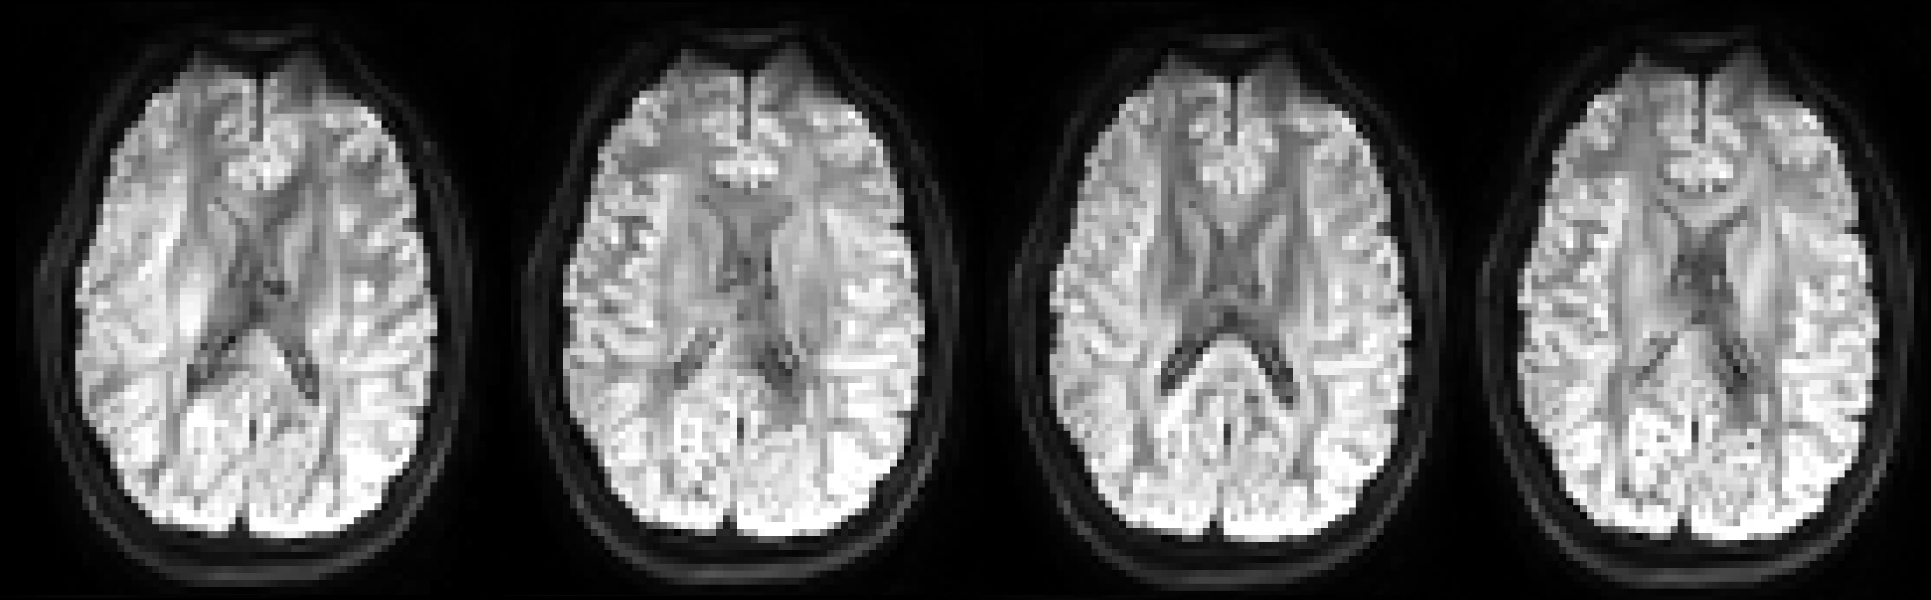
\includegraphics[width=0.95\textwidth]{./chapters/chp5/FIG/dwi.png}
\end{center}
\caption{Axial DTI slices measured with different b-vectors. The
  resolution in the DT image is typically lower (here, 96x96x50)
  compared to in the T1 images.}
\label{fig:chp5:DTIslices}
\end{figure}

\subsection{DTI reconstruction with \freesurfer}
\label{sec:chp-dti:freesurfer-dtrecon}

Next, we aim to reconstruct comprehensive DTI data from the volume,
b-value, and b-vector files using the \freesurfer{} command
\emp{dt\_recon}. The command takes an input volume (following
\emp{-{}-i}), b-vector and b-values files (following \emp{-{}-b}), an
output directory \emp{-{}-o} and the \emp{recon-all} subject id
\emp{-{}-s}. Within our book data directory \emp{dicom/ernie/DTI}, we
can launch the following commands:
\terminal{\$ export SUBJECTS\_DIR=my-freesurfer-dir \\
  \$ dt\_recon -{}-i dti.mgz -{}-b dti.bvals dti.voxel\_space.bvecs -{}-s ernie -{}-o \$SUBJECTS\_DIR/ernie/dti}
\noindent with \emp{my-freesurfer-dir} replaced by the FreeSurfer subjects
directory (e.g. \emp{freesurfer/} from the book data set).

This command produces multiple output files; including
\emp{tensor.nii.gz}, \emp{register.dat} and \emp{register.lta}. The
registration in \emp{dt\_recon} uses the registration command
\emp{bbregister} to register the DTI
data~\cite{freesurfer-wiki}. Files with the suffix .nii are in the
NIfTI format. Of these, \emp{tensor.nii.gz} is the spatially-varying
diffusion tensor. Further, an eigendecomposition of this tensor in
terms of spatially-varying eigenvalues $\lambda_1, \lambda_2,
\lambda_3$ and eigenvectors $v_1, v_2, v_3$ are given in the files
\emp{eigvals.nii.gz}, and \emp{eigvec1.nii.gz},\emp{eigvec2.nii.gz},
and \emp{eigvec3.nii.gz}.


\subsection{Mean diffusivity and fractional anisotropy}

In addition, \emp{dt\_recon} produces the NIfTI files
\emp{adc.nii.gz} and \emp{fa.nii.gz} for the mean (or apparent)
diffusivity (MD) and fractional anisotropy (FA), respectively. 
The mean diffusivity is given by 
\begin{equation}
  \rm{MD} = \frac{1}{3}(\lambda_1 + \lambda_2 + \lambda_3),   
\end{equation}
where $\{\lambda_i\}_i$ are the eigenvalues of the diffusion tensor.
and is associated to the volume file \emp{adc.nii.gz}. The fractional
anisotropy is defined~\cite{kindlmann2007geodesic} by
\begin{equation}
\rm{FA}^2 = \frac{1}{2} \frac{\lambda_1-\lambda_2)^2 
+ (\lambda_2 - \lambda_3)^2 + (\lambda_3 - \lambda_1)^2}{\lambda_1^2 
+ \lambda_2^2 + \lambda_3^2} 
%= \sqrt{3/2 \frac{ \sqrt{(dev(D_{ij}), dev(D_{ij}))}}{\sqrt{(D_{ij},D_{ij})}}}.
\end{equation}

\begin{figure}	
  \begin{center}
    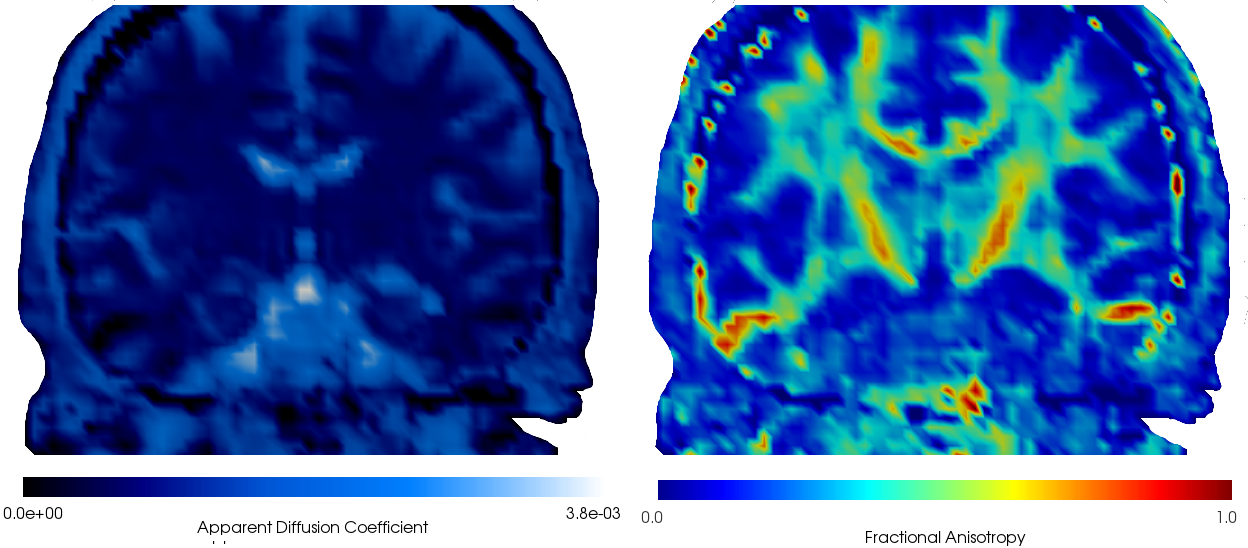
\includegraphics[width=0.95\textwidth]{./chapters/chp5/FIG/paraview_adcfa.png}
  \end{center}
  \caption{Mean diffusivity (left) and fractional anisotropy (right) as shown in \emp{Paraview}.}
  \label{fig:chp5:DTIfa}
\end{figure}
NIfTI files can be viewed in ParaView. You may first need to enable
the NIfTI viewer plugin by selecting the Paraview menu option
\button{Tools--Manage Plugins}, select the plugin option labeled
\button{AnalyzeNifTIIO} and then click \button{Load Selected}.  You
can then open and view (zipped) .nii files as you would any other
file in Paraview. Try opening the files \emp{adc.nii.gz} and
\emp{fa.nii.gz}; the results should look something like
Figure~\ref{fig:chp5:DTIfa}.

In general, the average FA is around 0.5 and changes by around 2\%
during day/night~\cite{voldsbekk2020evidence}; anisotropy decrease
with age, e.g.~around 14\% from 30 to 80
years~\cite{kochunov2011fractional}; and anisotropy can change up to
50\% in certain areas in an Alzheimer's disease patient compared with
healthy subjects~\cite{naggara2006diffusion}. In the \emp{ernie} data,
c.f.~Figure~\ref{fig:chp5:DTIfa}, the median white-matter FA value is
0.3, with a minimum of 0.009, and a maximum of 0.9998.
%% In closing, we
%% note that Eigenvalues computed by {\freesurfer} are sometimes
%% negative; clearly, this is not a physical result and DTI data must be
%% checked before it can be safely used in mathematical models.  Data can
%% be checked by opening the files, which all have self-explanatory
%% names, for the complete tensor, the eigenvalues and the eigenvectors.

\section{A finite element representation of the diffusion tensor}

In this section, we aim to
\begin{itemize}
\item
  improve on the DTI data to yield a valid eigendecomposition;
\item
  map the DTI tensor into a finite element tensor function defined on
  a finite element mesh;
\item
  briefly discuss co-registration.
\end{itemize}

\subsection{Preprocessing the diffusion tensor data}

The DTI data can be quite rough compared to the T1 data and our
corresponding finite element meshes. Moreover, the signal can be
disturbed close to the CSF, which makes the data in certain areas of
the cortical grey matter and in the regions near the ventricle system
less reliable. Indeed, inspection of the eigenvalues of the DTI tensor
shows non-physiological (zero and/or negative) eigenvalues. To ensure
a physiologically (and mathematically) reasonable diffusion tensor, we
recommend preprocessing the diffusion tensor prior to numerical
simulation. In particular, we here present two scripts that
\begin{itemize}
\item
  check the DTI tensor data for non-physiological values;
\item
  replaces non-physiological by physiological values in the DTI tensor,
\end{itemize}
respectively.

\subsubsection*{Creating brain masks}

To aid in this process, we will use \freesurfer{} to create so-called
masks of the brain i.e.~filters where voxels (significantly) outside
the brain are set to zero. Using our white matter parcellation data
(included in \emp{freesurfer/ernie/mri/wmparc.mgz}), brain masks can be
  created as follows:
\terminal{\$ mri\_binarize --i wmparc.mgz --gm --dilate 2 --o mask.mgz}
\noindent The \emp{dilate} determine how much the mask should be
extended outside the brain surface provided by
\emp{wmparc.mgz}. Examples of such masks are shown in
Fig.~\ref{fig:chp5:masks}.
\begin{figure}	
\begin{center}
  
\includegraphics[trim=400 130 500 150,clip,width=0.49\textwidth]{./chapters/chp5/FIG/mask0.png}
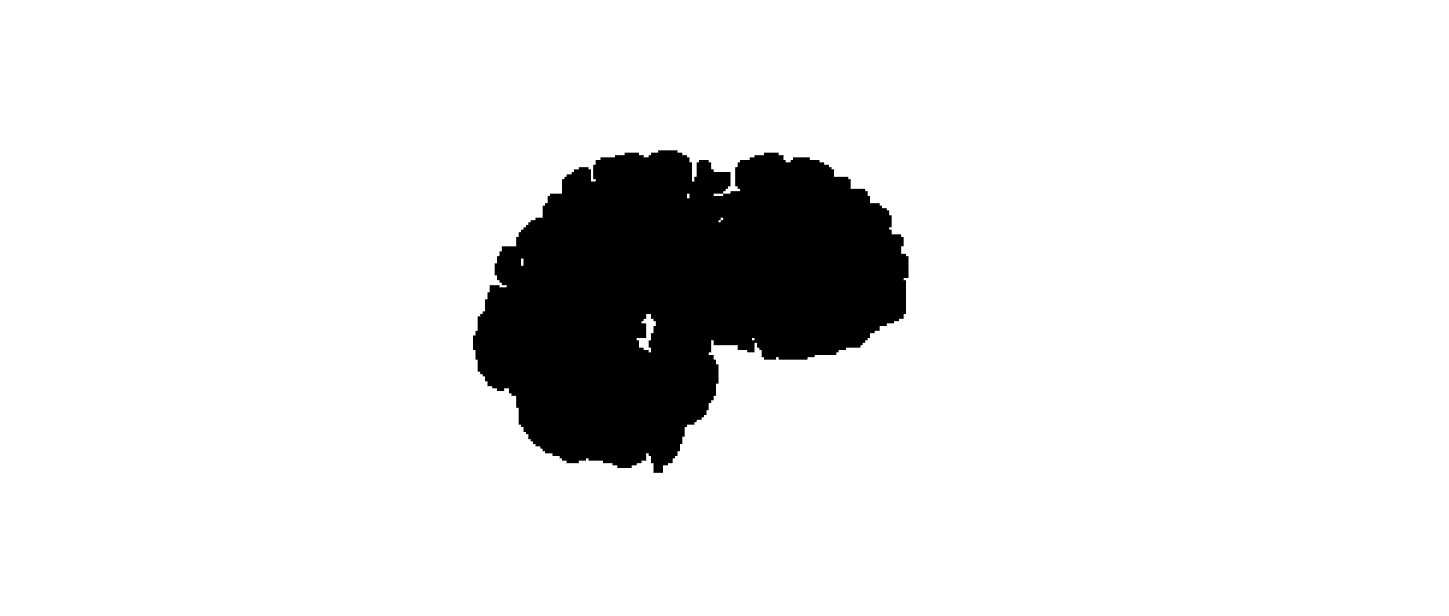
\includegraphics[trim=400 130 500 150,clip,width=0.49\textwidth]{./chapters/chp5/FIG/mask1.png} \\

\includegraphics[trim=400 130 500 150,clip,width=0.49\textwidth]{./chapters/chp5/FIG/mask2.png}
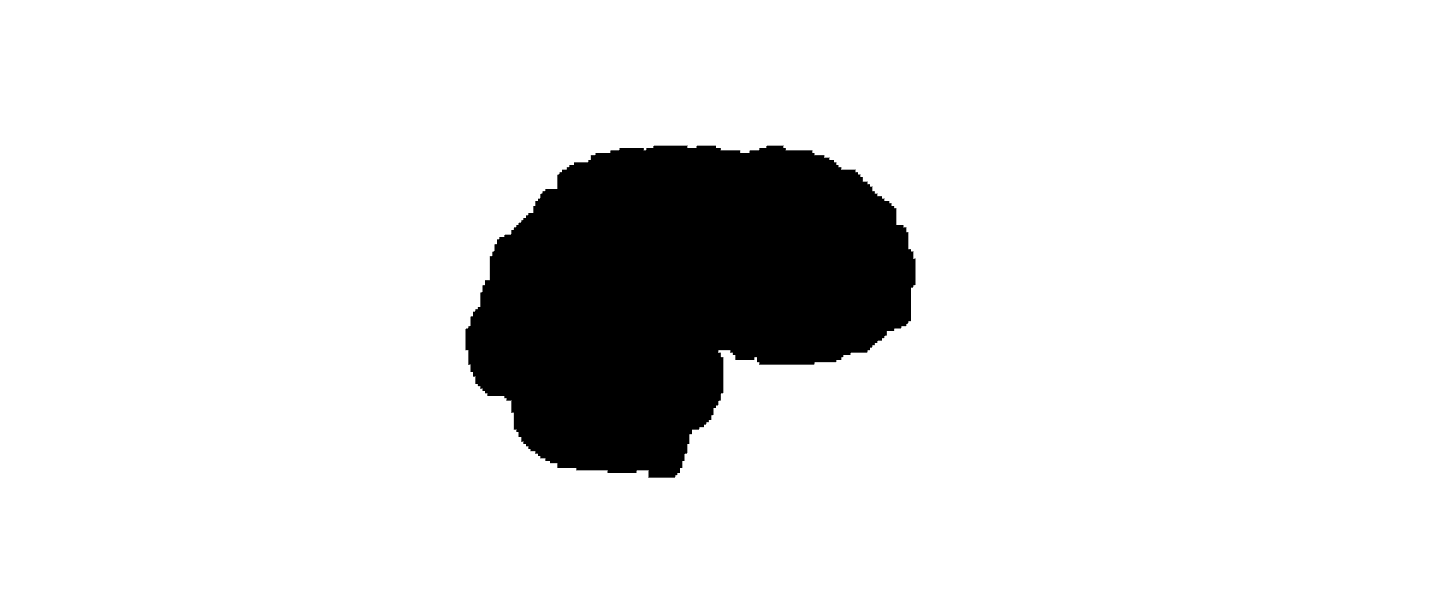
\includegraphics[trim=400 130 500 150,clip,width=0.49\textwidth]{./chapters/chp5/FIG/mask3.png}
\end{center}
\caption{
  Brain masks created using \emp{mri\_binarize} with \emp{dilate} ranging from 0 to 3.
}
\label{fig:chp5:masks}
\end{figure}

\subsubsection*{Examining the DTI data values}

We can work with the DT image data in a very similar manner as we did
for the parcellation (image) data in
Chapter~\ref{sec:chp4:mapping_parcellation}. We will again use NiBabel
to load the image data, use the \emp{vox2ras} functions for mapping
between the different image coordinate systems (DTI voxel space and T1
voxel space), and process the data as NumPy arrays. The complete
script can be run as:
\terminal{\$ cd mri2fem/chp5\\
\$ python3 check\_dti.py -{}-dti tensor.nii.gz -{}-mask mask.mgz}

We import the key packages:
\newpythonsnippet{chp5}{check_dti.py}{1}{6}

\noindent We define the function \emp{check\_dti\_data} that takes the DTI
tensor and mask files as input: 
\newpythonsnippet{chp5}{check_dti.py}{8}{20}

\noindent Now, the important coordinate transformations can be handled as follows:
\newpythonsnippet{chp5}{check_dti.py}{21}{30}

\noindent Before computing eigenvalues:
\newpythonsnippet{chp5}{check_dti.py}{33}{37}
and computing the fractional anisotropy and checking the validity of each voxel value:
\newpythonsnippet{chp5}{check_dti.py}{46}{58}

\subsubsection*{Improving the DTI values by extrapolation}
\mer{Lars: Could you check that the code examples run!! Something is amiss here.}

In the case that there are numerous invalid voxels, we can try
improving on the DTI data by extrapolating the adjacent valid
voxels. The complete
script can be run as:
\terminal{\$ cd mri2fem/chp5\\
\$ python3 clean\_dti\_data.py -{}-dti tensor.nii.gz -{}-mask mask.mgz -{}-out\_nii tensor-clean.nii}
\noindent and the main functionality reads as:
\newpythonsnippet{chp5}{clean_dti_data.py}{26}{48}

The function \pythoninline{find_valid_adjacent_tensor} will search for a valid
tensor in the adjacent voxel, and iteratively increase the search if
no valid tensor is found. We define a valid tensor
based on a non-zero sum of the MD. If there are multiple valid tensors within
the search, then the tensor with the MD closest to the median of non-zeros MD is
chosen.
\newpythonsnippet{chp5}{clean_dti_data.py}{7}{24}

\subsection{Representing the DTI tensor in \fenics{}}
\label{chp5:sec:loading-dti-tensor}

We are now ready to map our preprocessed DTI image (now in T1 voxel
space) onto a FEniCS mesh. We assume that we have a \emp{mesh}
available (for instance \emp{ernie-brain-32.h5} from
Chapter~\ref{chp4:meshio-converting}), that we have loaded the clean DTI
image and data in \emp{dti\_image} and \emp{dti\_data} and that that
we have the \emp{ras2vox} transform associated with this image:
\newpythonsnippet{chp5}{dti_data_to_mesh.py}{49}{51}

To represent the diffusion tensor in FEniCS, we create a FEniCS
\emp{Function} over a \emp{TensorFunctionSpace} of (discontinuous)
piecewise constant polynomial fields (\emp{"DG", 0}): 
\newpythonsnippet{chp5}{dti_data_to_mesh.py}{53}{55}

We could now extract the cell midpoints as we have done before, but we
can also extract the coordinates of the degrees of freedom of the
function space and convert these to voxel indices:
\newpythonsnippet{chp5}{dti_data_to_mesh.py}{57}{68}

We can now reshape the DTI data into a cell-wise structure,
\newpythonsnippet{chp5}{dti_data_to_mesh.py}{70}{72}
\noindent assign it to the FEniCS tensor field \pythoninline{D},
\newpythonsnippet{chp5}{dti_data_to_mesh.py}{78}{79}
and save it with the mesh: 
\newpythonsnippet{chp5}{dti_data_to_mesh.py}{87}{90}
The resulting fiber directions can be inspected in Figure~\ref{fig:chp5:freesurfer-parc}.
\begin{figure}	
  \begin{center}
  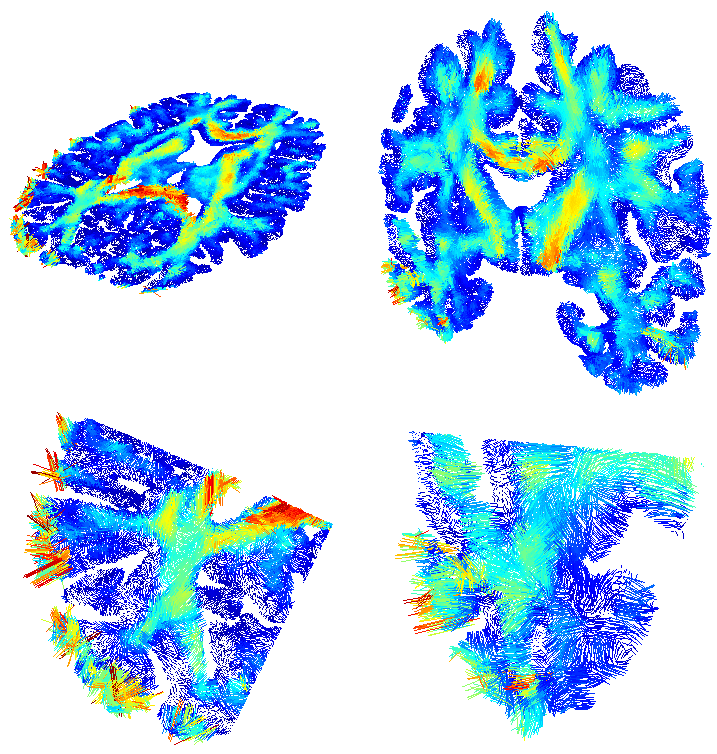
\includegraphics[width=0.8\textwidth]{./chapters/chp5/FIG/fiber-fa-2.png}
  \end{center}
\caption{Upper panels show fiber directions (DTI eigenvectors) colored
  by the fractional anisotropy in the axial and coronal plane. The
  lower panels show a zoom focusing on the boundary between grey
  matter and the CSF.}
\label{fig:chp5:freesurfer-parc} 
\end{figure}




%% We have added the function \pythoninline{adjusting_mean_diffusivity}, which allows the user to specify the minimum and maximum values inside a subdomain. The subdomains are determined by the tags set in {\svmtk} and any updates to the subdomains, like parcellations, that we mentioned in chapter \ref{sec:chp4:addparcellations}.

%% \pythonsnippet{chp5}{dti_data_to_mesh.py}{10}{31}

%% The function will first compute the MD, and then go through the input of limits. The limits is an Nx3 array, containing the subdomain label/tag, the lower and the upper MD limits. Setting either of the limits to zero will set the limits at infinity or minus infinity. This effectively cause the mask to be empty and thus having no effect on the data. 

%% We first sett the MD to 1 for all values outside the lower and upper limits. Then, the function will multiple the tensor with the appropriate limits. This can also be used to normalize the tensor based on the MD by setting both upper and lower limit equal to 1. In order to utilize this property, we can add Nx3 array to the function call like.
%% \begin{python}
%% dti_data_to_mesh("ernie.h5", "clean-dti-data.mgz","ernie.h5",[1,5.0e-5,1.0e-3])
%% \end{python}

%% We save the DTI tensor function together with the in a .h5 file, and we will use this tensor in the next chapter.
%% \pythonsnippet{chp5}{dti_data_to_mesh.py}{83}{95} 


\subsection{A note on co-registering DTI and T1 data}
\label{sec:chp-dti:freesurfer-coord}

As we have seen {\freesurfer} uses several different coordinate
systems for labeling the position of data in its various output
files. Thus, to combine data from different modalities, we need to
extract information about the different coordinate systems and be able
to map between these. This process is known as co-registration. We
have used NiBabel functionality to handle this process, but
include some additional information on co-registration here for context.

%% We aim to use our DTI data alongside the meshes and parcellations
%% created from the T1 images in the previous chapters. In order to do
%% so, we first need to consider co-registration -- a process that allows
%% us to transfer data between different {\freesurfer} output files. In
%% particular, {\freesurfer} uses several different coordinate systems
%% for labelling the position of data in its various output files, and
%% thus to combine data from different modalities, we need to be able to
%% map between the different coordinate systems. 

In short, let $x_1 = (x_1, y_1, z_1)$ and $x_2 = (x_2, y_2, z_2)$ represent the
same physiological point in $\R^3$ but represented with respect to two
different coordinate systems (bases). Then, there is an affine
transformation such that
\begin{equation} 
x_2 = A\, x_1 + b,
\end{equation}
for $A \in R^{3 \times 3}$ and $b \in \R^3$. Determining the
transformation matrix $A$ and vector $b$ for a pair of files is the
co-registration.

The key step in co-registration is to ascertain the type of coordinate system used 
for the files related to the T1 images, and those related to the DTI images. To 
to this end, we use the \emp{mri\_info} command. We begin by inspecting the T1 files:
\terminal{\$ cd \$SUBJECTS\_DIR/ernie/mri \\
\$ mri\_info orig.mgz -{}-orientation \\
LIA}
\noindent The output \emp{LIA}, above, means that the T1 image files
were generated with respect to the `Left Inferior Anterior' coordinate
system (see~\cite{freesurfer-wiki} for details).

To determine the DTI data coordinate system, we do the same for the
generated tensor NIfTI file:
\terminal{\$ cd \$SUBJECTS\_DIR/ernie/dti \\
\$ mri\_info tensor.nii.mgz -{}-orientation \\
LPS}
Let's break down the result of \emp{LPS}; the first letter determines the 
positive direction in the sagittal plane and can be either (L)eft or (R)ight; 
the second letter determines the positive direction in the coronal plane and 
can be either (P)osterior or (A)nterior; the third letter determines the positive 
direction in the axial plane and can be either (I)nferior and (S)uperior. 
Thus, the coordinate systems \emph{LIA} and \emph{LPS} differ by a choice of 
positive direction in the second and third axes. To co-register these images, 
then, we can swap the orientation of these two axes.

%% To close this section we provide an example of a transformation that could be 
%% used to convert imaging data from the so-called Voxelspace coordinate system 
%% to the so-called SurfaceRAS coordinate system; this is for illustration purposes 
%% to make the conversation concrete.  In a terminal type the following command 
%% \terminal{\smpprmpt{\emp{mri\_info} orig.mgz -{}-vox2ras-tkr}}
%% \noindent You will see the following output in the terminal window
%% \terminal{\outprmpt{
%% \begin{tabular}{rrrr}
%%   -1.00000   & 0.00000  &  0.00000 & 128.00000 \\
%%    0.00000   & 0.00000  &  1.00000 &-128.00000 \\
%%    0.00000   &-1.00000  &  0.00000 & 128.00000 \\
%%    0.00000   & 0.00000  &  0.00000 &   1.00000
%% \end{tabular}}}
%% \noindent  The above output means that if we wanted to convert coordinates expressed 
%% in terms of Voxelspace coordinates, $x_V = (x_V,y_V,z_V)$, to coordinates expressed 
%% in SurfaceRAS coordinates, $x_R = (x_R,y_R,v_R)$, we would use the transformation 
%% matrix $A$ and vector $b$ given by   
%% \[
%% A=\left[\begin{array}{ccc} -1 & 0 & 0 \\
%%                            0 & 0 & 1 \\
%%                            0 & -1 & 0
%% \end{array} \right], \quad \mbox{and} \quad  
%% b=\left[\begin{array}{c} 128  \\
%%                         -128  \\
%%                          128 
%% \end{array} \right], 
%% \]
%% and that the voxel dimension, indicated by the bottom-right output, is 
%% $1.0\times 1.0 \times 1.0$.  That is
%% \[
%% x_R = \left[\begin{array}{ccc} -1 & 0 & 0 \\
%%                            0 & 0 & 1 \\
%%                            0 & -1 & 0
%% \end{array} \right]\,x_V + \left[\begin{array}{c} 128  \\
%%                         -128  \\
%%                          128 
%% \end{array} \right].
%% \]  



%\section{XX TBD}

%We can see in Figure (insert DTI figure) that the diffusion tensor is a spacial variable, and as such we can define it as a \emp{Function} in FEniCS. In order to do this, we must first decide what type of element we should use to represent the tensor. We often consider tensors as cell data, therefore the selection of P0 seems to fit with diffusion elements.   

%(i.e. P0,P1 elements etc)  


%A general problem is that tetrahedrons in our mesh does not fit with the voxel data as shown in Fig. ??. This can be solved by utilizing different interpolation methods, 




%It should be noted that interpolation of tensor does not preserve the tensor properties, like anisotropy, so different interpolation methods are often used instead. 

%An example of this is the interpolation between bifurcation of an axon bundle in the white matter, see Fig ?? . The Euclidean interpolation will create a new tensor by averaging based on 
%\begin{equation}
%\mathbf{C}_{EL}(t) = (1-t)\mathbf{A} + t\mathbf{B} .
%\end{equation} 
%The resulting tensor will have a lower fractional anisotropy. 


%Therefore, we will introduce Linear Invariant(LI) interpolation. 
 






%On this mesh we may define a FEniCS tensor field $D$. However, a main problem is that this tensor field will be expressed in 
%the coordinate system of the mesh based on the T1 data, while we have the tensor field in 
%terms of another coordinate system. Hence, we will fetch the coordinates from the mesh, $x_{T1}$ and transform them 
%to the DTI based corresponding coordinates as $x_{T1} = A x_{DTI} + b$.  
%Then we may express $D(x_{DTI})$ which is simply \pythoninline{data} can be expressed in 
%terms of $D(x_{DTI}) = D(A^{-1}(x_{T1} - b))$. In other words, we extract the coordinates from the tensorfield made in FEniCS and
%transform them into the DTI coordinate system before we evaluate the DTI tensor. 
%
%Hence, we start by creating a  \pythoninline{TensorFunctionSpace} object. 
%The function \pythoninline{tabulate_dof_coordinates} provides us with the coordinates of each degree of freedom in this field. 
%The numbering is such that all dofs corresponding to the same cell is grouped together. For instance, the first 9 entries will contain identical 
%$\mathbb{R}^3$ vectors, namely the coordinates of the $3\times 3$ tensor of cell 0, before the next 9 entries which belongs to cell 1.      
%Hence, only every 9th coordinate will be unique. The following code re-shapes the coordinate into a suitable format. 
%\begin{python}
%DG0 = FunctionSpace(mesh, "DG",0)
%imap = DG0.dofmap().index_map()
%num_dofs_local =  imap.local_range()[1]-imap.local_range()[0]
%xyz = DG0.tabulate_dof_coordinates().reshape((num_dofs_local,-1))
%\end{python}
%Thus \emp{xyz} contains only one coordinate for each node, and we find the correspond voxel by applying the transformation matrix. 
%\begin{python}
%from nibabel.affines import apply_affine
%ijk = apply_affine(matrix,xyz).T
%i,j,k =np.rint(ijk).astype('int')  
%\end{python}
%It is encouraged to use \emp{paraview} to visually inspect that the transformation is suitable.   
%Below, we detail the various transformations. 
%
%First we look at the registration of DTI-images to T1-weighted images. This registration matrix can be found in the output folder of \emp{dt\_recon}, and if we provided the option \emp{-{}-lta} we might have two registration files. The default file is \emp{register.dat}, and as mentioned before, it contains the transformation matrix for registration in the Surface RAS coordinates. The optional registration file will have the filename provided with the option \emp{-{}-lta}, which we called \emp{registration.lta}. This registration file has the transformation matrix of the registration in voxelspace coordinates. Thus, the two registration files have different approach to obtain the complete transformation matrix.  
%The registration matrix can be obtained from the \emp{.dat} text file with the following function.
%\begin{python}
%def load_registration_dat(filename):
%    import numpy as np
%    with open(filename, 'r') as f:
%         matrix = np.array([i.strip(" \n").split(" ") 
%                  for i in f.readlines()[4:8]],dtype='float32')   
%    return matrix
%\end{python}      
%We can similarly obtain the registration matrix from \emp{.lta} text file using the function. 
%\begin{python}
%def load_registration_lta(filename}
%    import numpy as np
%    with open(filename, 'r') as f:
%         matrix = np.array([i.strip(" \n").split(" ") 
%                     for i in f.readlines()[8:12]],type='float32')   
%    return matrix
%\end{python}  
%\lmv{ no longer needed, as we use nibabel function resample\_from\_to. Thus we only need to read from the header vox2ras\_tkr, but I feel it should be here to illustrate the need for transformation. }  
% 
%We can now read the registration matrices into python with the provided function, so the next step is determine the complete transformation matrix. In our case, we want to obtain the transformation matrix from Surface RAS to DTI-voxelspace. There are two options, depending on which registration file is chosen, to construct the complete transformation matrix. Both options require that we obtain a transformation matrix from Surface-RAS to voxelspace, which is know as \emp{vox2ras\_tkr}.
%
%There are different methods to obtain the \emp{vox2ras\_tkr} affine matrix. The first method  is to obtain it from the header of a mgz-file.
%\begin{python}
%import nibabel as nb
%dti    = nb.load("orig.mgz")
%header = dti.header  
%vox2ras_tkr = header.get_vox2ras_tkr()
%\end{python}
%A more explicit implementation reads, 
%\begin{python}
%def get_vox2ras_tkr(t1):
%    ds = t1.header._structarr['pixdim'][1:4]
%    ns = t1.header._structarr['dim'][1:4] * ds / 2.0
%    v2rtkr = np.array([[-ds[0], 0, 0, ns[0]],
%                       [0, 0, ds[2], -ns[2]],
%                       [0, -ds[1], 0, ns[1]],
%                       [0, 0, 0, 1]], dtype=np.float32)
%    return v2rtkr
%    
%dti    = nb.load("tensor.nii.gz") 
%vox2ras_tkr = get_vox2ras_tkr(dti)
%\end{python}
%
%We are now ready to define the complete transformation matrix, form Surface-RAS to DTI-voxelspace. If we use \emp{registration.dat}, we need to invert the registration matrix in order to transform from Surface-RAS to DTI-Surface-RAS. Then we multiple with the inverted vox2ras\_tkr so that we can go from DTI-Surface-RAS to DTI-voxelspace.
%\begin{python}
%# dat file  contains is RAStkr(SurfaceRAS) to 
%# RAStkr  affine transformation matrix 
%regdat = load_registration_dat(filename)
%vox2ras = get_vox2ras_tkr(dti)
%matrix = np.linalg.inv(get_vox2ras_tkr(dti)).dot(regdat)   
%\end{python}
%If we use \emp{registration.lta}, we need to invert the transformation matrix from voxelspace and Surface-RAS. This is then multiplied with the inverted registration matrix so that we go from voxelspace to DTI-voxelspace.  
%\begin{python}      
%# lta file contains  vox2vox affine transformation matrix
%reglta = load_registration_lta(filename )
%vox2ras = orig.header.get_vox2ras_tkr()
%matrix = np.linalg.inv(vox2ras.dot(reglta)) 
%\end{python}
%
%It is worth mentioning that the transformation between coordinate system can have some problems with out of bounds voxels. In other words, the mesh can have some coordinates that corresponds to voxelspace that do not exists in the DTI-voxelspace. We can solve this by actively setting the coordinates to be within the bounds of the voxelspace. 
%\begin{python}
%i[data.shape[0]<=i]=data.shape[0]-1
%j[data.shape[1]<=j]=data.shape[1]-1
%k[data.shape[2]<=k]=data.shape[2]-1
%\end{python}






















\chapter{Simulating anisotropic diffusion in heterogeneous brain regions}
\label{chp:chp6}

In this chapter, we return to our model problem~\eqref{eq:diffusion}
and bring together the different tools and techniques introduced in
Chapters~\ref{chp:chp3} to \ref{chap:dti}. The computational domain
will be determined from T1-weighted data and divided into grey and
white matter subdomains, diffusion tensor imaging (DTI) data will be
employed in the construction of the heterogeneous and anisotropic
diffusion tensor, and specific sub regions, such as the hippocampus,
will be selected to assess site-specific solute distribution governed
by a diffusive process.

In practice, one should first address data and mesh resolution
issues. For instance, raw DTI data can exhibit rough transitions, as
well as noise. This is particularly true in the grey matter proximal
to cerebrospinal fluid (e.g.~Figures~\ref{fig:chp5:DTIfa} and
\ref{fig:chp5:freesurfer-parc} in Chapter \ref{chap:dti}). Here, we assume that 
the DTI data have been suitably smoothened and denoised for use in simulations. In
addition, we must ascertain a mesh resolution that is suitable to
provide reliable estimates of the spread  of different
molecules, while avoiding the unnecessary computational costs
associated with over-resolving the mesh.

\section{Molecular diffusion in one dimension}
\label{sec:chp6:1D-tests}

\index{amyloid-beta}
To estimate a suitable spatial mesh resolution, time step, and time scale of the solute diffusion, it is useful to
first consider equation \eqref{eq:diffusion} in one dimension for different
molecules. Here, we consider the protein fragment amyloid-beta
(A$\beta$) associated with neurodegenerative
disease~\cite{iliff2012paravascular}, the tracer gadobutrol used in
glymphatic magnetic resonance imaging~\cite{ringstad2018brain}, and water. The
effective diffusion coefficient $D$ in brain tissue for each of these
molecules is estimated to be $6.2 \times 10^{-5}$ mm$^2$/s,
$1.3 \times 10^{-4}$ mm$^2$/s, and $1.1 \times 10^{-3}$ mm$^2$/s,
respectively~\cite{waters2010concentration,valnes2020apparent}.

\subsection{Analytical solution}
In one dimension and over the domain $(0, \infty)$, the parabolic
diffusion problem \eqref{eq:diffusion} with $u_0(x)=0$, $u(0, t) = 1$,
and $u(\infty, t) = 0$ allows for a simple analytic solution:
\begin{equation}
  \label{eq:analytical:1D}
  u(x,t) =  \mbox{erfc}(x / (2 \sqrt{D t})). 
\end{equation}

Figure~\ref{fig:chp6:analytics} shows solutions
of~\eqref{eq:analytical:1D} zoomed in on the (left) first 2 mm of the domain, 
and the (middle) first 10 mm after 9 hours, and (right) the first 10 mm after 24
hours. It is evident that diffusion is a slow process:
significant concentration changes occur within 2 mm of the boundary
after 9 hours; however, 1 cm away, the heavier molecules,
amyloid-beta and gadobutrol, still have concentrations near zero. The
source code for generating these plots is available in
\emp{mri2fem/chp6/analytical\_1D.py}.
\begin{figure}	
  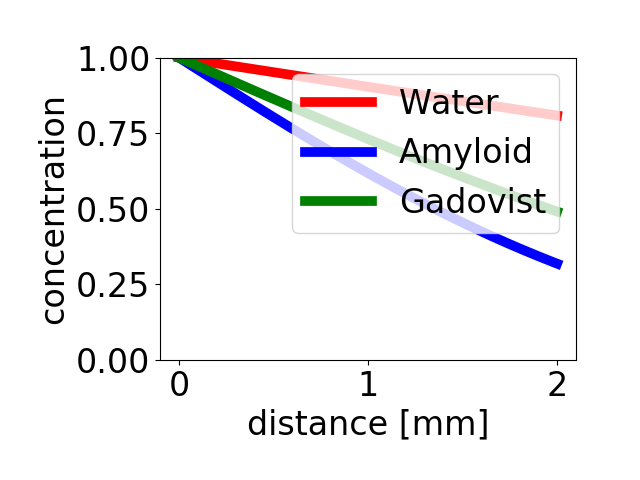
\includegraphics[width=0.32\textwidth]{./graphics/chp6/9hours_2mm_WAG}
  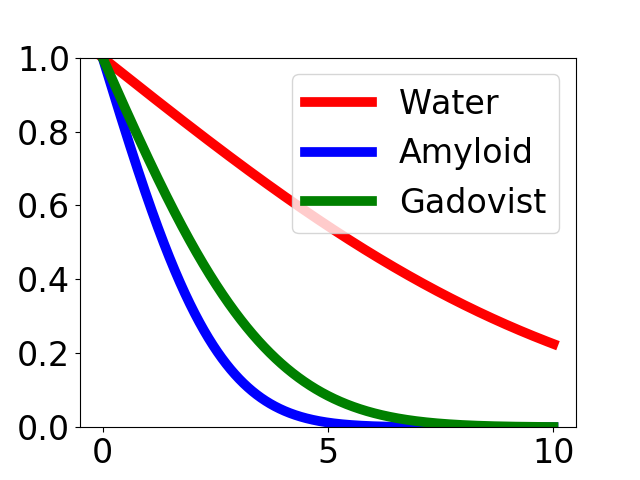
\includegraphics[width=0.32\textwidth]{./graphics/chp6/9hours_1cm_WAG}
  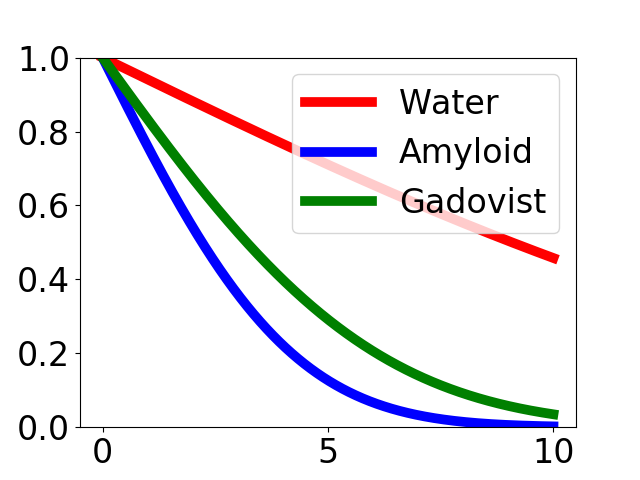
\includegraphics[width=0.32\textwidth]{./graphics/chp6/24hours_1cm_WAG}
  \caption{Diffusion according to \eqref{eq:analytical:1D}:
    concentration (arbitrary unit) versus distance from the
    source/left boundary  after 9 hours (left and middle) and
    after 24 hours (right).}
  \label{fig:chp6:analytics}
\end{figure}

\subsection{Numerical solution and handling numerical artifacts}
\index{mass lumping}
Next, we discretize \eqref{eq:diffusion} using the finite element
method (as described in Chapter~\ref{chp:chp3}). Note, however, that the
sharp change in the boundary versus initial conditions for our model
problem can lead to artificial oscillations in the numerical
solution. Such oscillations often diminish with refinement; they can
also be avoided through the use of monotonic or maximum principle
preserving schemes. Another common method, which we consider here, for
Galerkin finite element schemes is mass lumping (%
e.g.~\cite{langtangen2016solving}). We provide FEniCS-based source
code for the finite element solution of~\eqref{eq:diffusion} with and
without mass lumping in \emp{mri2fem/chp6/diffusion\_1D.py}. To use
this script, see, for example 
\terminal{\$ cd mri2fem/chp6 \\
\$ python3 diffusion\_1D.py -{}-help}
\begin{figure}	
\subfigure[$t=30$ minutes, standard Galerkin]{ 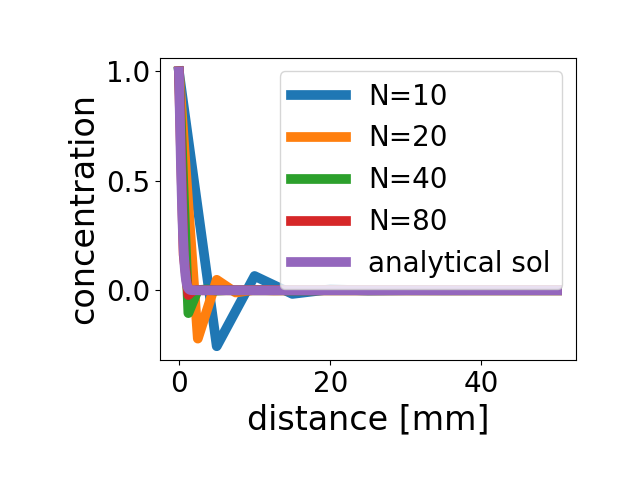
\includegraphics[width=0.49\textwidth]{./graphics/chp6/Amyloid_numerical_1D_L_max50_dt300_final1800_lumpednot.png}}
\subfigure[$t=30$ minutes, lumped mass matrix]{ \includegraphics[width=0.49\textwidth]{./graphics/chp6/Amyloid_numerical_1D_L_max50_dt300_final1800_lumpedlumped.png}} \\
\subfigure[$t=9$ hours, standard Galerkin]{ \includegraphics[width=0.49\textwidth]{./graphics/chp6/Amyloid_numerical_1D_L_max50_dt300_final32400_lumpednot.png}}
\subfigure[$t=9$ hours, lumped mass matrix]{ \includegraphics[width=0.49\textwidth]{./graphics/chp6/Amyloid_numerical_1D_L_max50_dt300_final32400_lumpedlumped.png}}
\caption{
  Comparison of standard Galerkin (left) and mass-lumped (right)
  finite element schemes of the diffusion
  equation~\eqref{eq:diffusion} in one dimension over $\Omega = (0, 50)$
  mm at different times. The parameter $N$ is the number of finite elements and the time step is 5 minutes. }
\label{fig:chp6:numerics}
\end{figure}

The standard and mass-lumped finite element solutions are shown in
Figure~\ref{fig:chp6:numerics} at different times and with different
time steps. Early, for coarse resolutions ($N = 10$ or $N=20$), with mesh size parameter $h=50 \, \mbox{mm}/N$,  the
standard approach yields considerable nonphysical oscillations, whereas 
the mass-lumped solution (right) produces significant numerical
diffusion. However, in the longer term context, the standard Galerkin
scheme is clearly desirable: the former allows for a spatial
resolution of $N=10$ or $N=20$, whereas the latter requires $N=40$ or
$N=80$ to control the numerical diffusion. Essentially, the initial
error from the short-term Gibbs phenomena, that is, the discontinuous
initial data, is no match for the long-term regularizing effect of the
parabolic partial differential equation. Therefore, these early errors do not contribute much to the
long-term numerical solution.

In conclusion, these results suggest that, if we are interested in
long-term dynamics, a time step size of $\Delta t \approx$ 5 minutes with
a spatial resolution of $N=40$ or $N=80$, corresponding roughly to a
quasi-uniform mesh cell diameter of $0.5$ mm $\leq h \leq 1$ mm, is
a good starting target for the standard Galerkin approach in our three dimensional 
(3D) discretization. The corresponding scheme with a lumped mass matrix does however
significantly overestimate the diffusion at $N=80$. 

\section{Anisotropic diffusion in 3D brain regions}

In this section, we consider simulations of gadobutrol diffusion 
and compute the average concentrations in different brain regions. In
particular, we begin with the following steps:
\begin{itemize}
\item
  We create a brain mesh with grey and white matter marked and
  ventricles removed and mark parcellation regions as described in
  Chapter~\ref{chp4:parcellations}. 
\item
  We filter and map our DTI data onto this geometry as described in 
  Chapter~\ref{chp5:sec:loading-dti-tensor}.
\item
  Using FEniCS, we implement a version of the diffusion simulation
  script presented in
  Chapter~\ref{sec:chp3:fenics-code-implementation} allowing for
  anisotropic diffusion and the computation of integrals over labeled
  regions.
\end{itemize}
In the numerical simulation, we represent the DTI data in the form of
a heterogeneous and anisotropic diffusion tensor field $D$. The FEniCS
code for setting up the diffusion tensor field reads 
\newpythonsnippet{chp6}{chp6-diffusion-mritracer.py}{35}{38}

\index{FEniCS!integrating over regions}
\noindent We compute the average amount of tracer in a labeled region by
integrating the concentration over the region and dividing by the
region's volume as follows (with the regions labeled 17 and 1035 as
examples):
\newpythonsnippet{chp6}{chp6-diffusion-mritracer.py}{151}{152}

\noindent The precise commands run are included in
\emp{mri2fem/chp6/all.sh}, and the script
\emp{mri2fem/chp6/chp6-diffusion-mritracer.py} gives the complete
FEniCS code.

\subsection{Regional distribution of gadobutrol}
We compute the average concentrations of gadobutrol diffusing in from
the brain's surface in regions 17 (hippocampus), 1035 (insula grey
matter), 3035 (insula white matter), 1028 (superior frontal grey
matter), and 3028 (superior frontal white matter).  Gadobutrol has a
diffusivity approximately twice that of amyloid-beta, and the
estimated mesh size and time step of the previous section should therefore apply
to this case as well.  The resulting curves are shown in
Figure~\ref{chp6:regions}, and the simulations results are shown in
Figures~\ref{fig:chp6:numerics4}--\ref{fig:chp6:numerics5}. Note that, here, 
we consider the tracer distribution in certain regions as a
function of time; the distribution therefore starts at a low value and increases 
with time as the solute diffuses throughout the brain. Clearly, the
distribution of gadobutrol in the grey matter regions and hippocampus
are affected much more than in the white matter regions. This result is
expected since both the grey matter and hippocampus are
closer to the cerebrospinal fluid where, in our simulation, the gadobutrol
concentration is assumed to reside initially.  It is also observed
that the upper regions, that is, the superior frontal grey and white matter
(1028 and 3028, respectively), experience faster gadobutrol deposition
than the corresponding regions on the side of the brain.
\begin{figure}%[t]
  \centering
  \includegraphics[width=0.7\textwidth]{./graphics/chp6/tracer_uniform_notlump_regions_64.png}
  \caption{Average concentration of gadobutrol (y-axis, arbitrary
    unit) versus time (x-axis, hours) in different brain regions: 17
    (hippocampus), 1035 (insula grey matter), 3035 (insula white
    matter), 1028 (superior frontal grey matter), and 3028
    (superior frontal white matter). Time step: 6 minutes, $N=64$ brain
    mesh (cf.~below).}
  \label{chp6:regions}
\end{figure}
%\begin{figure}	
%  \includegraphics[width=0.49\textwidth]{./graphics/chp6/Gadovist_slice_subdomain.png}
%  \includegraphics[width=0.49\textwidth]{./graphics/chp6/Gadovist_slice_9hours.png}
%  \caption{
%    The mesh and subdomains for the mesh with resolution parameter set to 32 (left)  
%    and the simulated distribution of Gadobutrol after 
%    9 hours (right).}
%  \label{fig:chp6:numerics4}
%\end{figure}

\begin{figure}	
  \includegraphics[width=0.98\textwidth]{./graphics/chp6/Image1.png}
  \caption{
    The simulated distribution of gadobutrol, for a mesh with resolution parameter set to 32, after 0 hours (left), %
    after 5 hours (middle) and after 9 hours (right).}
  \label{fig:chp6:numerics4}
\end{figure}
\begin{figure}	
  \includegraphics[width=0.90\textwidth]{./graphics/chp6/Image2.png}
  \caption{Illustration of the simulated distribution of solute
    concentration in the brain within the cranium.}
  \label{fig:chp6:numerics5}
\end{figure}



\subsection{Accuracy and convergence of computed quantities} 

\index{mesh convergence}
A common question and topic in numerical simulations is whether the
computed solutions have converged.  We therefore investigate next the mesh
convergence of the standard Galerkin and mass-lumped Galerkin
approaches. More precisely, we consider a set of meshes, aiming to 
determine the 
%
%of increasing
%resolution and compare the quantities computed on the different meshes
%aiming for determining 
accuracy of the numerical solution. In this
example, we consider a roughly uniform refinement, but the mesh is not
refined in place; rather, a sequence of meshes is first generated at
different resolutions using the surface volume meshing toolkit (\svmtk). In particular, 
we construct a sequence of quasi-uniform meshes, as follows (using 
\emp{mri2fem/chp6/create\_mesh\_refinements.py}):
\index{mesh refinement!uniform}
\newpythonsnippet{chp6}{create_mesh_refinements.py}{0}{100}

After creating the meshes we mark the subdomains of interest and map the DTI data onto the mesh, before 
running the simulations. The following is a code snippet from \emp{mri2fem/chp6/all.sh} that shows how
the 16 mesh is created by the scripts described in the previous chapters: 
\begin{lstlisting}[style=bashStyle]
# using the 16 mesh 
# convert to h5
python3 ../chp4/convert_to_dolfin_mesh.py \
   --meshfile brain_16.mesh --hdf5file brain_16.h5

# mark subdomains  
python3 ../chp4/add_parcellations.py \
    --in_hdf5 brain_16.h5 \
   --in_parc ../chp4/wmparc.mgz \
   --out_hdf5 brain_16_tags.h5 \
   --add 17 1028 1035 3028 3035

# add dti to the h5 file 
python3 ../chp5/dti_data_to_mesh.py  \
   --dti ../chp5/clean-dti.mgz \
   --mesh brain_16_tags.h5 --label 1 0.4 0.6 \
   --out DTI_16.h5 

# run simulation 
python3 chp6-diffusion-mritracer.py --mesh DTI_16.h5 \
   --lumped lumped --annotation uniform16lumped 
python3 chp6-diffusion-mritracer.py --mesh DTI_16.h5 \
   --lumped not --annotation uniform16notlumped 
\end{lstlisting}


The average gadobutrol concentrations in the hippocampus over time
for the sequence of meshes generated here are shown in
Figure~\ref{fig:chp6:numerics2}, without (left) and with (right)
mass lumping. Clearly, the standard Galerkin approach (left) seems to
yield more consistent results than the mass-lumped Galerkin scheme
(right). However, even for the standard Galerkin scheme, whether the
solutions are fully converged  seems questionable at the highest
resolution tested (around 15.5 million mesh cells). Recall that piecewise
constants are used to represent the anisotropic diffusion tensor $D$.
This DG construction requires about nine entries per cell, thus yielding
approximately 140 million values for 15.5 million cells. Higher resolutions, such
as those for piecewise linear or quadratic constructions, are not
feasible on a personal computing device with only 32 gigabytes of RAM.
\begin{figure}	
  \includegraphics[width=0.49\textwidth]{./graphics/chp6/tracer_hippocampus_uniform_notlump.png}
  \includegraphics[width=0.49\textwidth]{./graphics/chp6/tracer_hippocampus_uniform_lump.png}
  \caption{Average gadobutrol concentration in the hippocampus (y-axis,
    arbitrary unit) versus time (x-axis, hours) for different mesh
    resolutions, $\Delta t = 6$ min. Quasi-uniform mesh sequence with
    $N=16$, $32$, $64$, $128$ generated by \svmtk. Standard Galerkin (left)
    versus mass-lumped Galerkin (right) discretizations.}
\label{fig:chp6:numerics2}
\end{figure}

\index{mesh refinement!adaptive}
To further assess the accuracy and convergence of the computed
concentrations under mesh refinements, we therefore also consider
adaptively refined meshes. In particular, we focus on the hippocampus
and adaptively refine the meshes in this region, starting from the
$N=16$ brain mesh of the previous mesh sequence. Again, we plot the
average gadobutrol concentrations in the hippocampus over time for
a sequence of adaptively refined meshes (see
Figure~\ref{fig:chp6:numerics3} with (right) and without (left)
mass-lumping). Using this technique, we find the solutions between the first, second,
and third adaptive refinements differ little for the standard
scheme. However, mesh convergence for the mass-lumped Galerkin
strategy remains unclear, even after four refinements to the
hippocampal region.  

Finally, we examine the mesh statistics (e.g.~the number 
of vertices, cells and the range of mesh sizes) for the uniformly and 
adaptively refined meshes.  Before doing so, we comment on the variables 
$h$, $h_{\text{max}}$ and $h_{\text{min}}$.  In the field of scientific 
computing, $h$ typically refers to a quantity defined on each tetrahedron $T$ 
in the mesh and $h =h_T= \max\left\{x-y\right\}$ where $x$ and $y$ are any two 
points in $T$.  We can then define the max and min values as 
$h_{\text{max}} = \max{h_T}$ and $h_{\text{min}}$ is defined similarly; the 
$T$ subscript on $h_T$ is typically dropped and we have 
$h_{\text{min}} \leq h \leq h_{\text{max}}$.  Figure~\ref{fig:chp6:numerics2} 
suggests that, on quasi-uniform meshes, we reach mesh convergence around the 
refinement level denoted by `128' which, by Table~\ref{chp6:meshstat} (left), 
consists of about 15.5 million tetrahedrons.  Figure~\ref{fig:chp6:numerics3} 
suggests that when we use adaptive refinement, mesh convergence is reached at 
refinement level `4' which, by  Table~\ref{chp6:meshstat} (right), consists of 
nearly 7.7 million tetrahedrons.  Thus, adaptive refinement has reduced the 
number of mesh tetrahedrons by half; a clear benefit.  Using our one-dimension 
test case, in Chapter~\ref{sec:chp6:1D-tests}, we estimated a value of 
$h_\text{min}\approx 0.5\text{mm}$ would be needed to reach mesh convergence. 
However, the results of Table~\ref{chp6:meshstat} indicate that our estimate 
was off by a factor of about $3$, for the quasi-uniform case, or $10$, for the 
adaptive case.  
\begin{figure}	
\includegraphics[width=0.49\textwidth]{./graphics/chp6/tracer_hippocampus_notlumped_addaptive.png}
\includegraphics[width=0.49\textwidth]{./graphics/chp6/tracer_hippocampus_lumped_addaptive.png}
  \caption{Average gadobutrol concentration in the hippocampus
    (y-axis, arbitrary unit) versus time (x-axis, hours) for a
    sequence of adaptively refined meshes, $\Delta t = 6$
    minutes. Standard Galerkin (left) versus mass-lumped Galerkin (right)
    discretizations.}
\label{fig:chp6:numerics3}
\end{figure}

\begin{table}%
  \centering
  \begin{minipage}{.45\textwidth}%
    \begin{tabular}{l|cccc}
      Refinement & Vertices & Cells  & $h_{\min}$ & $h_{\max}$ \\ \hline
      16 & 94K & 457K & 0.97 & 11.4 \\  
      32 & 194K & 908K &  0.46 & 5.7 \\  
      64 & 567K &  2.75M & 0.26 & 2.9 \\
      128 &  2.8M & 15.5M &  0.14 & 1.45
    \end{tabular}
    %\label{tab:uniref}
  \end{minipage}%
  \hspace{2em}
  \begin{minipage}{.45\textwidth}%
    \begin{tabular}{c|cccc}
	    Refinement & Vertices & Cells & $h_{\min}$ & $h_{\max}$ \\ \hline
	     1 & 99K &  479K &  0.64 &  11.4 \\
	     2 & 123K& 613K & 0.30 &  11.4 \\
	     3 & 275K &  1.5M  &  0.14 & 11.4 \\
	     4 & 1.3M &  7.7M  & 0.07 &  11.4 \\
    \end{tabular}
    %\label{tab:localref}
  \end{minipage}%
%
  \caption{Mesh statistics (number of vertices, cells, and minimal and
    maximal cell sizes) for the (left) uniformly refined and
    (right) adaptively refined mesh sequences.}
  \label{chp6:meshstat}
\end{table}

In summary, we have established that assessing the process of tracer
distribution within the brain due to diffusion is a feasible, but
somewhat computationally demanding task. In our case, we focused on
the hippocampus and Gadobutrol enrichment and found that indeed a
standard Galerkin procedure was sufficient given a locally refined
mesh of a few hundred thousand cells. Quasi-uniform meshes on the
other hand needs several million cells before convergence. We also
remark that mass-lumping schemes, which are often prefered due to
their monotonic properties that reduce non-physical oscillations on
the short-term, is suffering from significant added numerical
diffusivity and corresponding non-physical spread of tracer in
long-term scenarios.


\newpage

\backmatter
\printindex

\bibliographystyle{siamplain}
\bibliography{bibliography}

\end{document}





